% section | subsection | subsubsection | paragraph | subparagraph | verbatim | enumerate | item

% Just let it be an Article bro
\documentclass{article}

% Cover Metadata
\title{Advanced Data Modelling}
\date{11 Nov 2025}
\author{Maulana Hafidz Ismail}

% Equation Setup
\usepackage{amsmath}

% Image Setup
\usepackage{graphicx}
\usepackage{float}

% Link Setup
\usepackage{hyperref}

% Highlighting Setup
\usepackage{soul}
\usepackage{xcolor}
\sethlcolor{red!30}
\newcommand{\hlblue}[1]{\sethlcolor{cyan!30}\hl{#1}\sethlcolor{yellow}}

% Line Width
\sloppy
\setlength{\emergencystretch}{3em}
\hbadness=99999

% Code Syntax Setup
\usepackage{listings}
\usepackage{xcolor} % untuk warna
\lstset{
basicstyle=\ttfamily\small,
frame=single,
breaklines=true,
backgroundcolor=\color{gray!10},
keywordstyle=\color{blue},
commentstyle=\color{gray},
stringstyle=\color{red},
tabsize=2,
captionpos=b
}

% Start of the Article
\begin{document}

% Cover Page
\pagenumbering{gobble}
\maketitle
\newpage

% Table of Content Page
\tableofcontents
\newpage
\pagenumbering{arabic}

% Main Content
\section{Data Modeling and Management}
\subsection{Pengenalan Pemodelan Data}
Data Model adalah representasi visual dari elemen data yang berbeda dan bagaimana mereka saling berhubungan.

\subsection{Tingkatan Model Database}
\begin{itemize}
    \item Conceptual Data Model: Model yang menggambarkan struktur data secara umum tanpa detail teknis.
    \item Logical Data Model: Model yang lebih terperinci yang menunjukkan bagaimana data akan disimpan dalam database.
    \item Physical Data Model: Model yang menggambarkan bagaimana data akan disimpan secara fisik dalam sistem.
\end{itemize}

\subsection{Normalisasi Database}
Normalization adalah proses untuk mengatur data dalam database untuk mengurangi redundansi dan menghindari anomali.
\begin{itemize}
    \item Insertion Anomaly: Kesulitan dalam menambahkan data baru karena ketergantungan pada data lain.
    \item Update Anomaly: Masalah yang muncul saat memperbarui data yang terduplikasi.
    \item Deletion Anomaly: Kehilangan data penting saat menghapus data yang tidak relevan.
\end{itemize}

\subsection{MySQL Workbench}
\begin{itemize}
    \item MySQL Workbench: Alat visual untuk pemodelan dan manajemen database.
    \item Forward Engineering: Proses mengubah model data menjadi skema database di MySQL.
    \item Reverse Engineering: Proses membuat model data dari database yang sudah ada.
\end{itemize}

\subsection{Data Warehousing}
\begin{itemize}
    \item Data Warehouse: Repositori data terpusat yang mengintegrasikan dan menyimpan data dari berbagai sumber.
    \item ETL (Extract, Transform, Load): Proses untuk mengambil data dari sumber, mengubahnya, dan memuatnya ke dalam data warehouse.
    \item Data Marts: Subset dari data warehouse yang berfokus pada area bisnis tertentu.
\end{itemize}

\subsection{Pemodelan Data Dimensional}
\begin{itemize}
    \item Dimensional Data Modeling: Teknik pemodelan yang menggunakan dimensi dan fakta, biasanya dalam bentuk skema bintang (star schema) atau skema salju (snowflake schema).
    \item Grain: Tingkat detail yang ditentukan dalam model data.
\end{itemize}

\subsection{Analisis Data}
Data Analytics adalah proses menganalisis data untuk mendapatkan wawasan.
\begin{itemize}
    \item Quantitative Data: Data yang dapat diukur dan dinyatakan dalam angka.
    \item Qualitative Data: Data yang bersifat deskriptif dan tidak dapat diukur dengan angka.
\end{itemize}

\subsection{Alat Analisis Data}
\paragraph{Tableau} adalah alat untuk visualisasi data yang memungkinkan pengguna untuk membuat dashboard interaktif dan menganalisis data secara mendalam.

\subsection{Pemodelan Data}
\begin{itemize}
    \item Pemodelan data memberikan representasi visual dari elemen data dan menunjukkan bagaimana mereka saling berhubungan. Ini membantu memahami bagaimana data disimpan, diakses, diperbarui, dan ditanyakan dalam basis data.
    \item Pemodelan data digunakan untuk mengembangkan berbagai jenis basis data, terutama entity relational databases, yang direncanakan dengan menggunakan \verb|entity relationship diagram (ERD)|.
\end{itemize}

\subsection{Tingkat Pemodelan Data}
\begin{itemize}
    \item Conceptual Data Model: Model ini memberikan gambaran umum yang tinggi tentang elemen data yang disebut entities. Tujuannya adalah untuk menunjukkan hubungan antara entitas dalam basis data. Contoh entitas untuk \verb|M&G| adalah pelanggan, produk, dan pesanan.
    \item Logical Data Model: Model ini lebih rinci dan mencakup atribut dari setiap entitas, mendefinisikan primary keys, dan spesifikasi foreign keys. Misalnya, client ID adalah primary key untuk tabel klien, dan menghubungkan tabel klien dengan tabel pesanan melalui foreign key client ID.
    \item Physical Data Model: Model ini digunakan untuk membuat skema SQL internal dari basis data. Ini mencakup fitur seperti datatypes, constraints, dan atribut. Contohnya, mendefinisikan datatype seperti varchar untuk atribut nama lengkap dan integer untuk nomor kontak. Constraints seperti \verb|NOT NULL| juga diterapkan untuk memastikan setiap kolom berisi data.
\end{itemize}

\subsection{Tipe-tipe Data Model}
Model data memberikan representasi visual dari elemen-elemen data dan menggambarkan bagaimana mereka saling berhubungan. Model ini memberikan pemahaman kepada insinyur basis data tentang cara data disimpan, diakses, diperbarui, dan diinterogasi dalam basis data.

Terdapat beberapa jenis model data yang dapat digunakan untuk merancang sistem basis data. Pilihan model yang digunakan sebaiknya didasarkan pada kesesuaiannya dalam mendukung kebutuhan bisnis.

\subsubsection{Model Data Relasional}
Model ini merepresentasikan basis data sebagai kumpulan relasi, di mana setiap relasi disajikan dalam bentuk tabel yang menyimpan informasi dalam baris dan kolom.

Keuntungan: Lebih sederhana digunakan dibandingkan model lain, memudahkan identifikasi dan akses data.

\subsubsection{Model Entity Relationship}
Model ini mirip dengan model relasional, tetapi setiap tabel dipresentasikan sebagai entitas terpisah dengan atributnya sendiri.

Model hubungan entitas biasanya digambarkan dalam diagram ER yang menampilkan entitas-entitas dalam basis data dan hubungan-hubungan yang berbeda di antara mereka, di mana setiap entitas memiliki kumpulan atribut yang terkait.

Model ini juga menggambarkan berbagai jenis multiplisitas, termasuk satu-ke-satu, satu-ke-banyak, dan banyak-ke-banyak.

Diagram ER berikut ini menggambarkan sistem pemesanan janji operasi. Sistem ini terdiri dari empat entitas: Dokter, Operasi, Janji, dan Pasien.

Setiap entitas memiliki kumpulan atribut, dan semua entitas terhubung melalui kunci asing. Menurut diagram ini:
\begin{itemize}
    \item Seorang pasien dapat membuat satu atau beberapa janji temu.
    \item Beberapa janji temu dapat ditugaskan kepada setiap dokter.
    \item Beberapa janji temu berlangsung di sebuah klinik tertentu.
\end{itemize}

Model data hubungan entitas mendukung persyaratan data operasi, dan diagram ER menampilkan struktur database secara mudah digunakan, sehingga Anda dapat menggunakannya untuk mendokumentasikan database Anda dan berkomunikasi tentang strukturnya dengan pemangku kepentingan Anda.

Anda juga dapat membuat diagram ini dalam alat pengembangan terintegrasi seperti MySQL Workbench dan mengimplementasikan model database secara langsung di MySQL.

\begin{figure}[H]
    \centering
    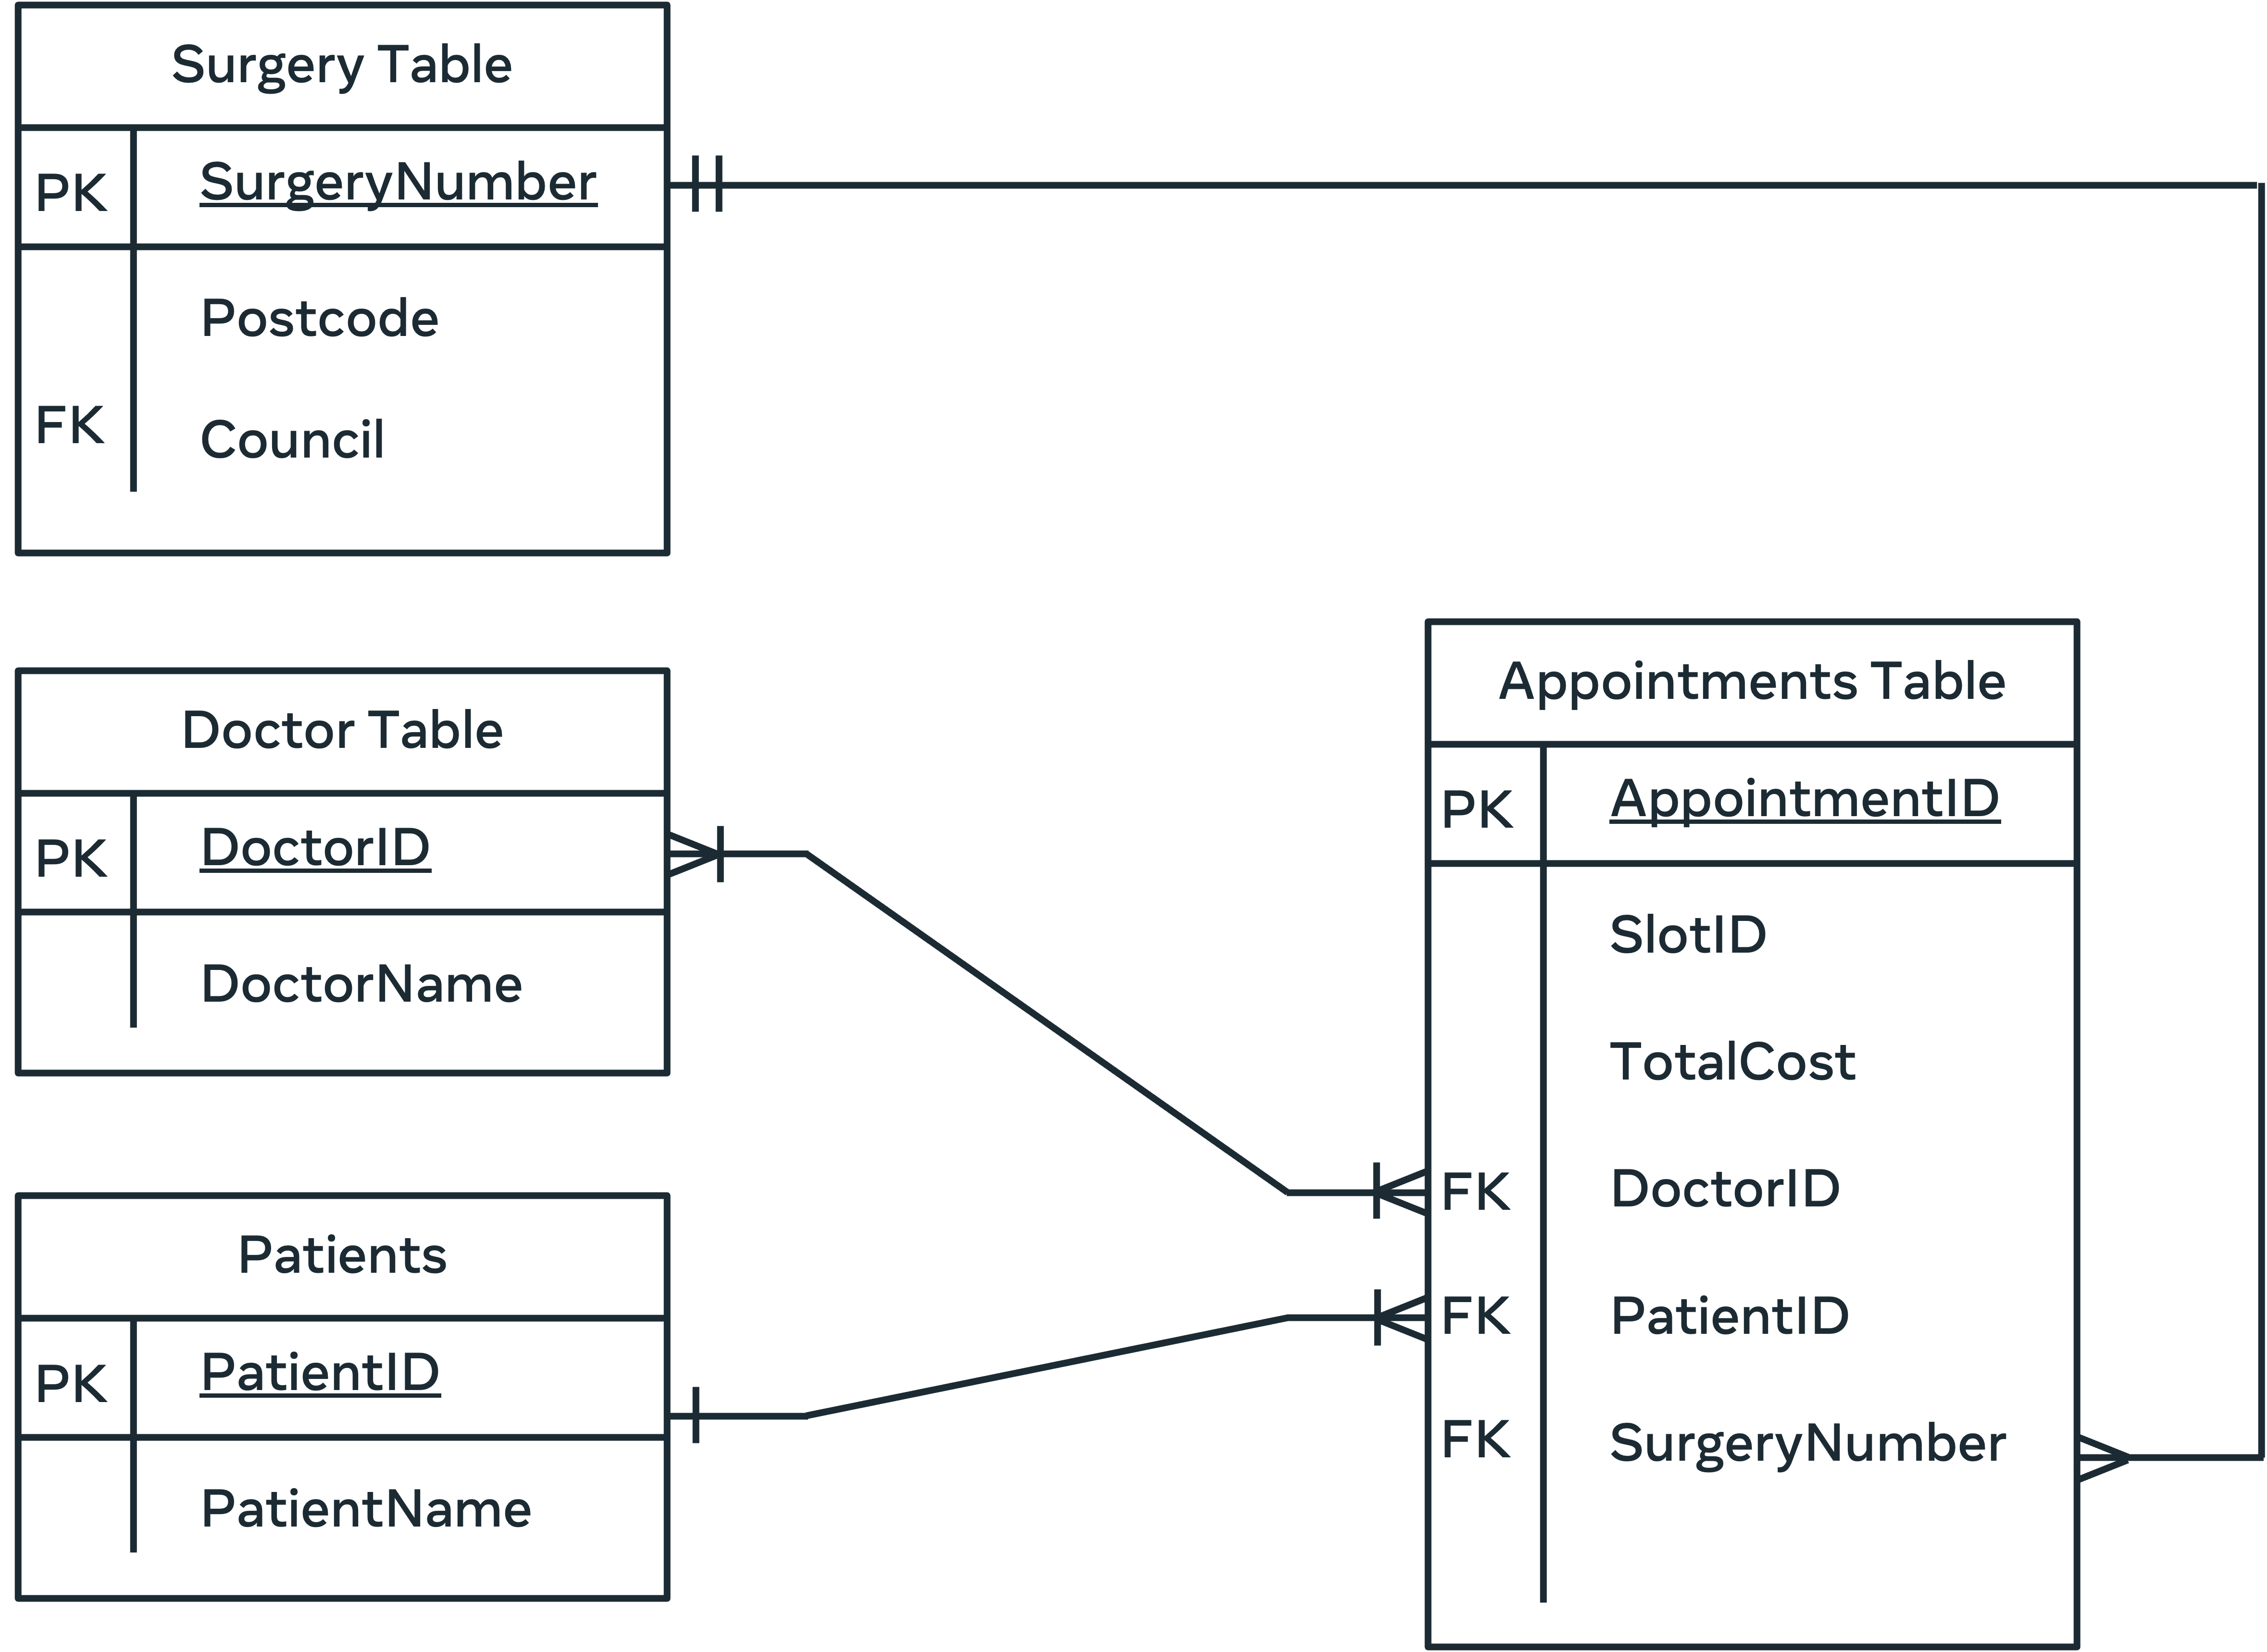
\includegraphics[width=0.8\textwidth]{./Picts/erd.png}
    \caption{}
\end{figure}

\subsubsection{Model Data Hierarkis}
Model ini mengorganisir data dalam struktur pohon (tree-like) dengan hubungan parent-child.

Hanya dapat merekam hubungan one-to-many, di mana setiap child node hanya dapat memiliki satu parent node.

Model data berikut ini menggambarkan struktur database perusahaan asuransi. Dalam diagram ini, perusahaan asuransi disusun sebagai berikut:
\begin{itemize}
    \item Departemen adalah node akar,
    \item Node Agen dan Staf terhubung ke node akar Departemen.
    \item Dan node Komputer dan Ketenagakerjaan terhubung ke node akar Staf.
\end{itemize}

\begin{figure}[H]
    \centering
    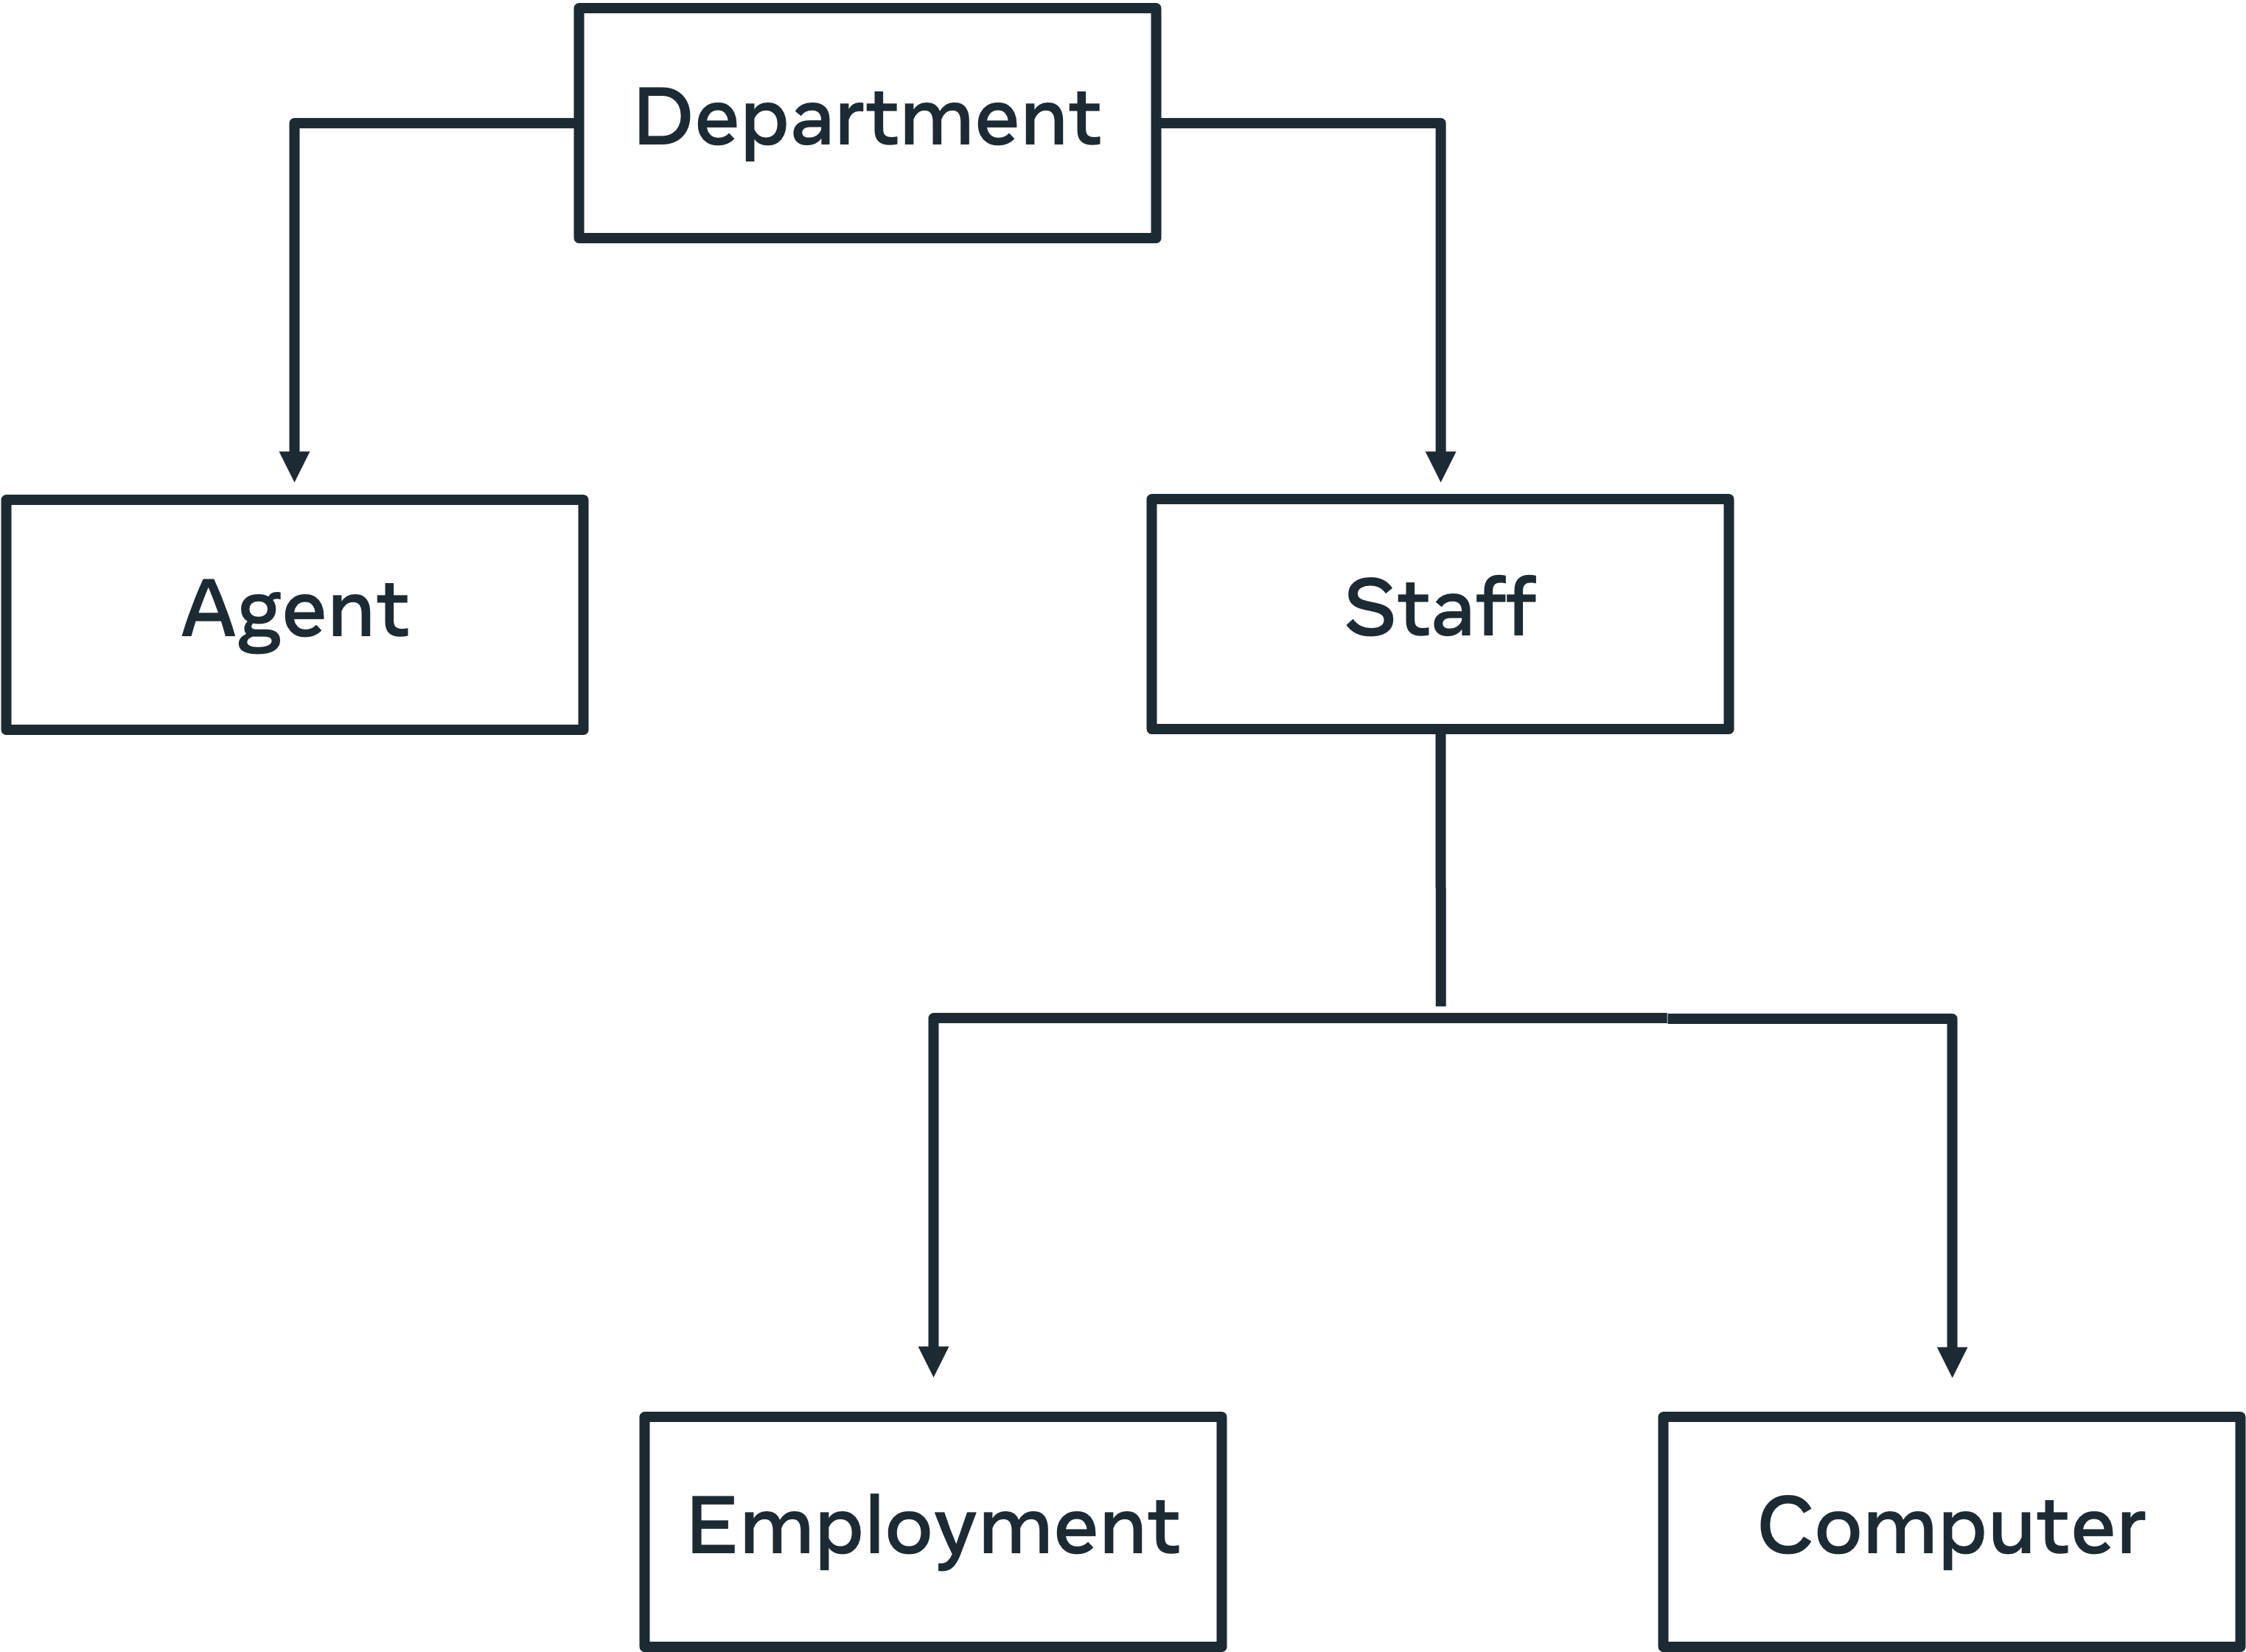
\includegraphics[width=0.8\textwidth]{./Picts/hirar.png}
    \caption{}
\end{figure}

Anda mungkin telah memperhatikan bahwa salah satu keunggulan utama model ini adalah kesederhanaan strukturnya. Selain itu, karena setiap catatan hanya memiliki satu induk, Anda dapat menavigasi basis data dengan cepat dan efisien. Namun, Anda perlu menyadari bahwa dalam model ini, jika Anda menghapus node induk, maka catatan anak yang terkait juga akan dihapus.

Selain itu, model ini tidak mendukung hubungan banyak-ke-banyak, yang mungkin diperlukan dalam beberapa kasus (seperti dalam skenario operasi sebelumnya).

Sulit juga untuk merestrukturisasi struktur basis data untuk mengakomodasi persyaratan baru. Melakukannya dapat mengganggu hubungan orang tua-anak yang sudah ada.

Anda dapat menggunakan diagram ER untuk mewakili tingkat detail yang lebih tinggi dari model ini seperti yang ditunjukkan di bawah ini.

\begin{figure}[H]
    \centering
    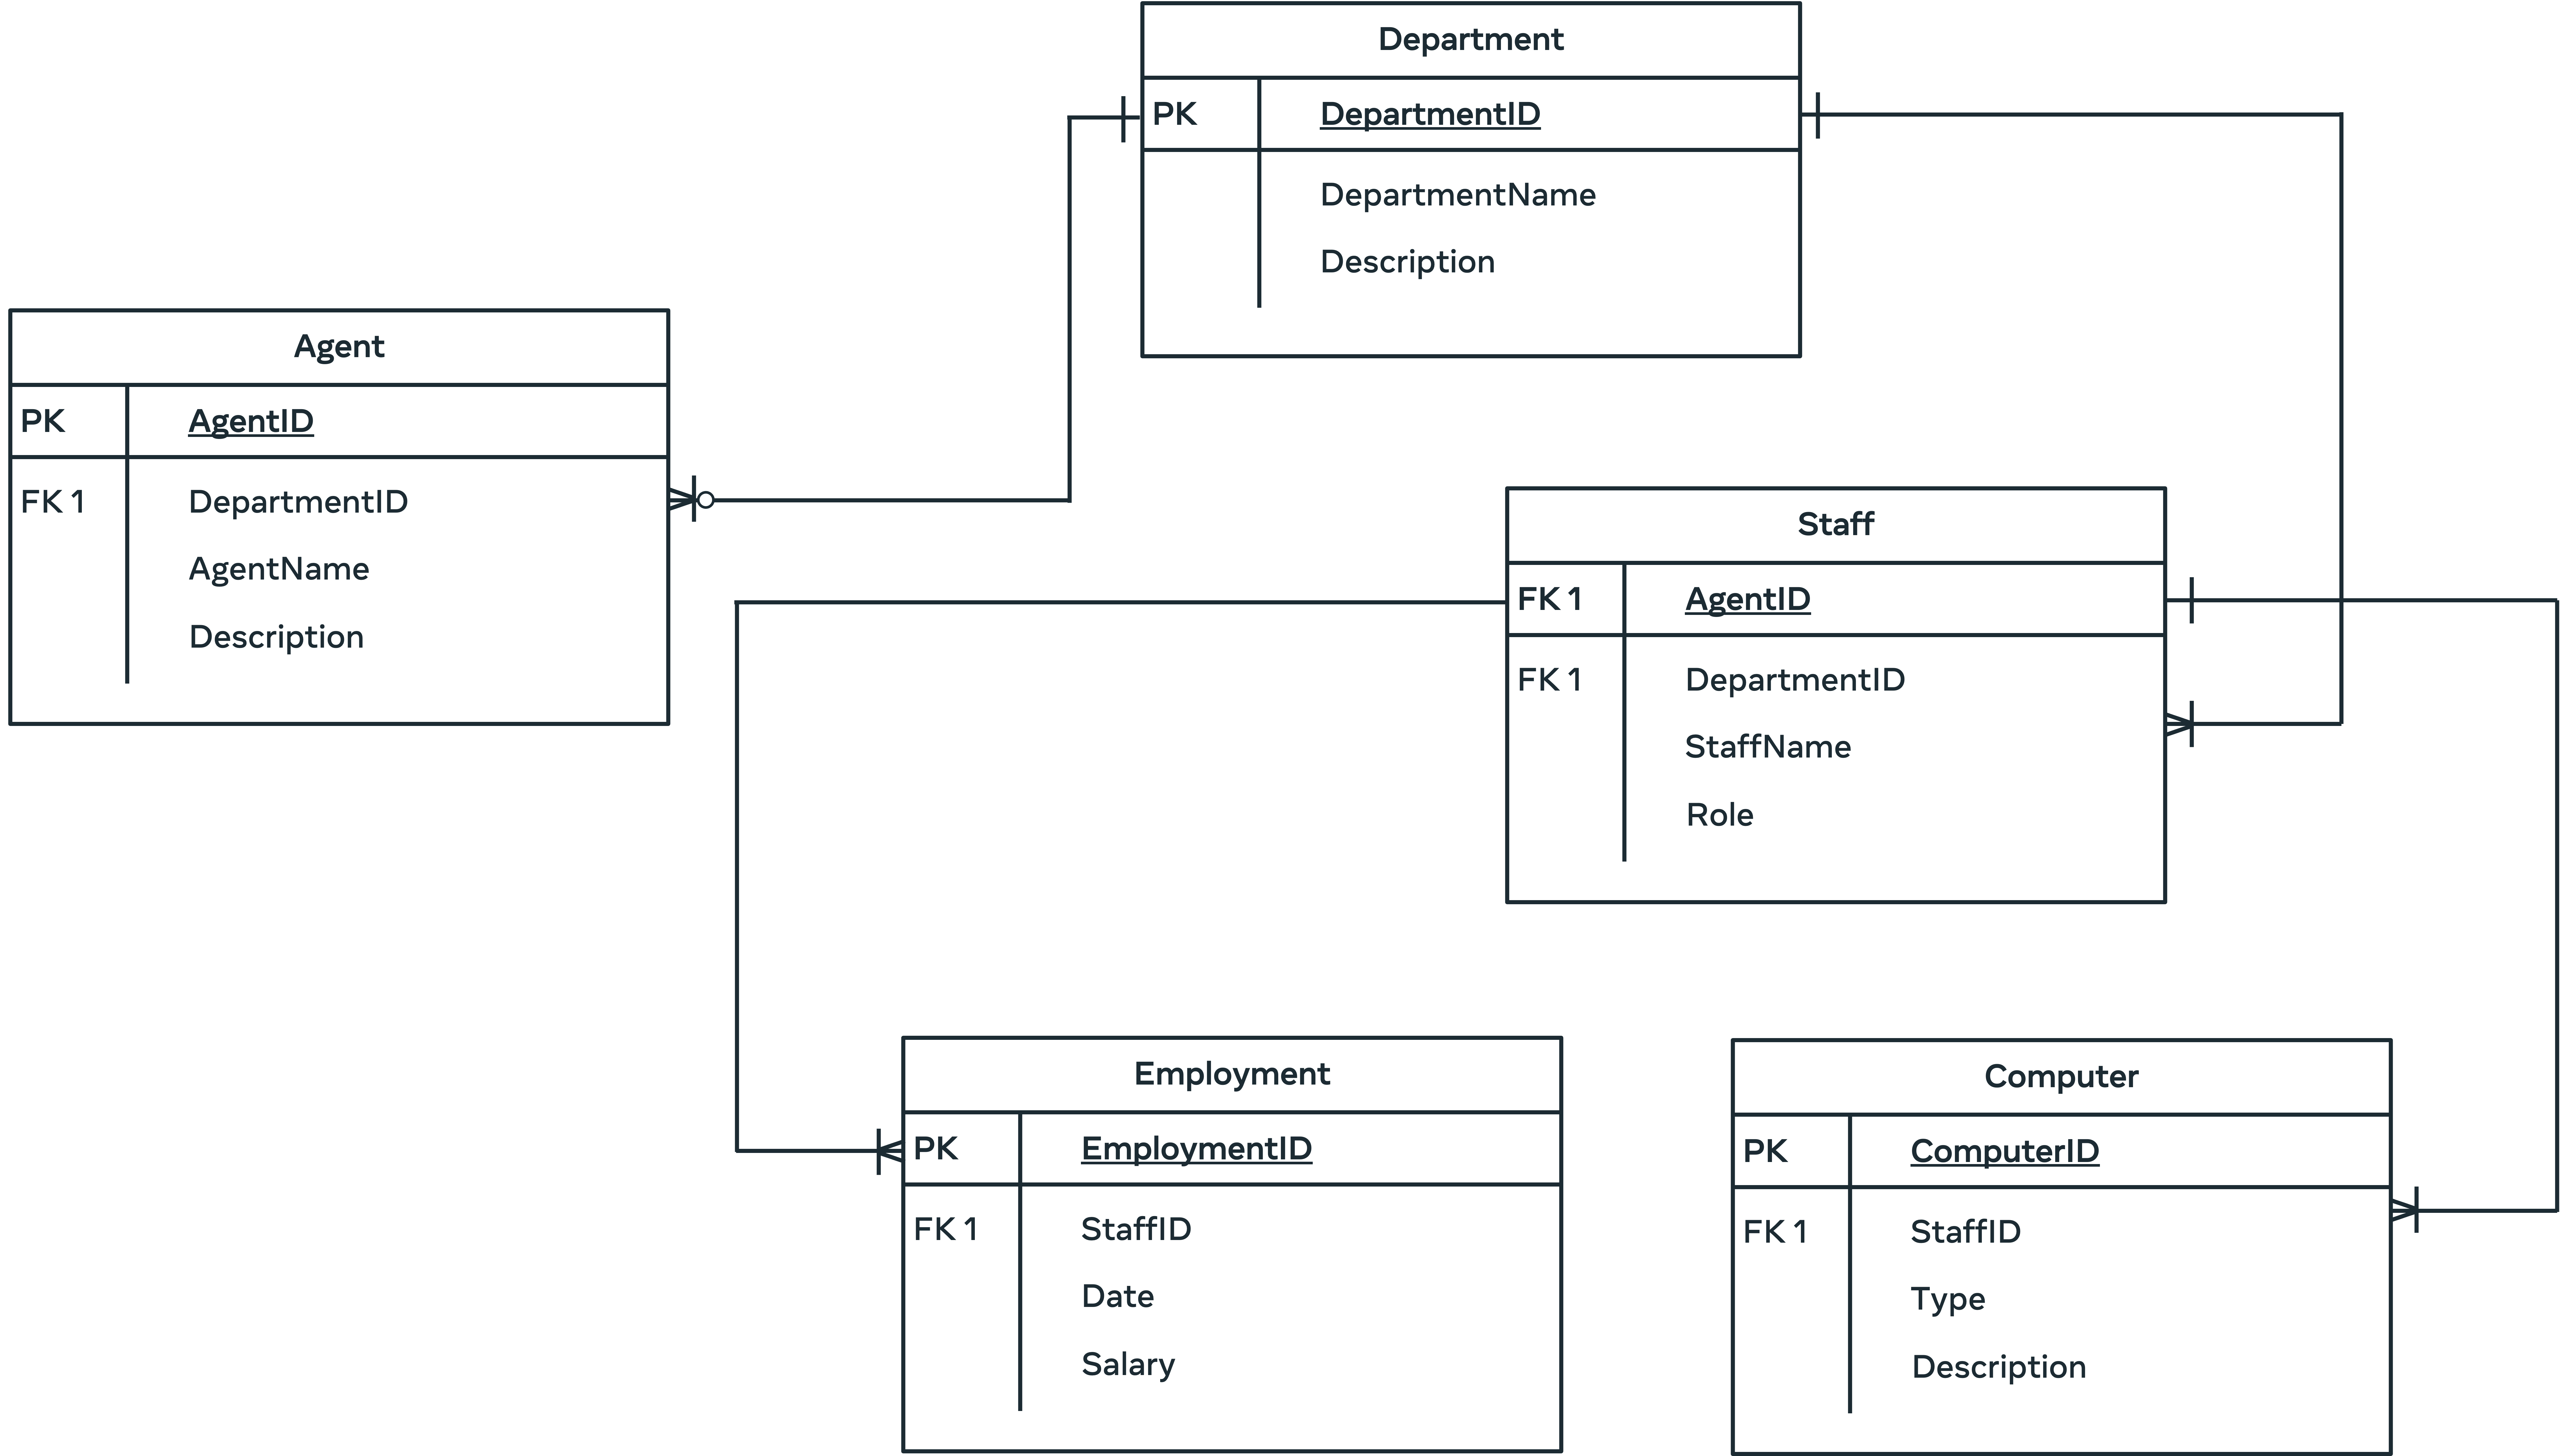
\includegraphics[width=0.8\textwidth]{./Picts/erdofhirar.png}
    \caption{}
\end{figure}

\subsubsection{Model Object Oriented}
Model ini berdasarkan konsep berorientasi objek (Object Oriented), di mana setiap objek diterjemahkan menjadi kelas yang mendefinisikan karakteristik  dan perilakunya.

Dalam model ini, Anda dapat menggunakan berbagai jenis hubungan antara objek, seperti agregasi, komposisi, dan pewarisan. Fitur-fitur ini membuat basis data berorientasi objek cocok untuk proyek yang kompleks. Namun, penggunaan model ini memerlukan pemahaman yang baik tentang pemrograman berorientasi objek.

Dalam diagram pendaftaran kursus berikut, terdapat enam kelas:
\begin{itemize}
    \item Person,
    \item Student,
    \item Professor,
    \item Course,
    \item Address
    \item dan Enrolment.
\end{itemize}

Setiap kelas terdiri dari sekumpulan atribut dan metode.

\begin{figure}[H]
    \centering
    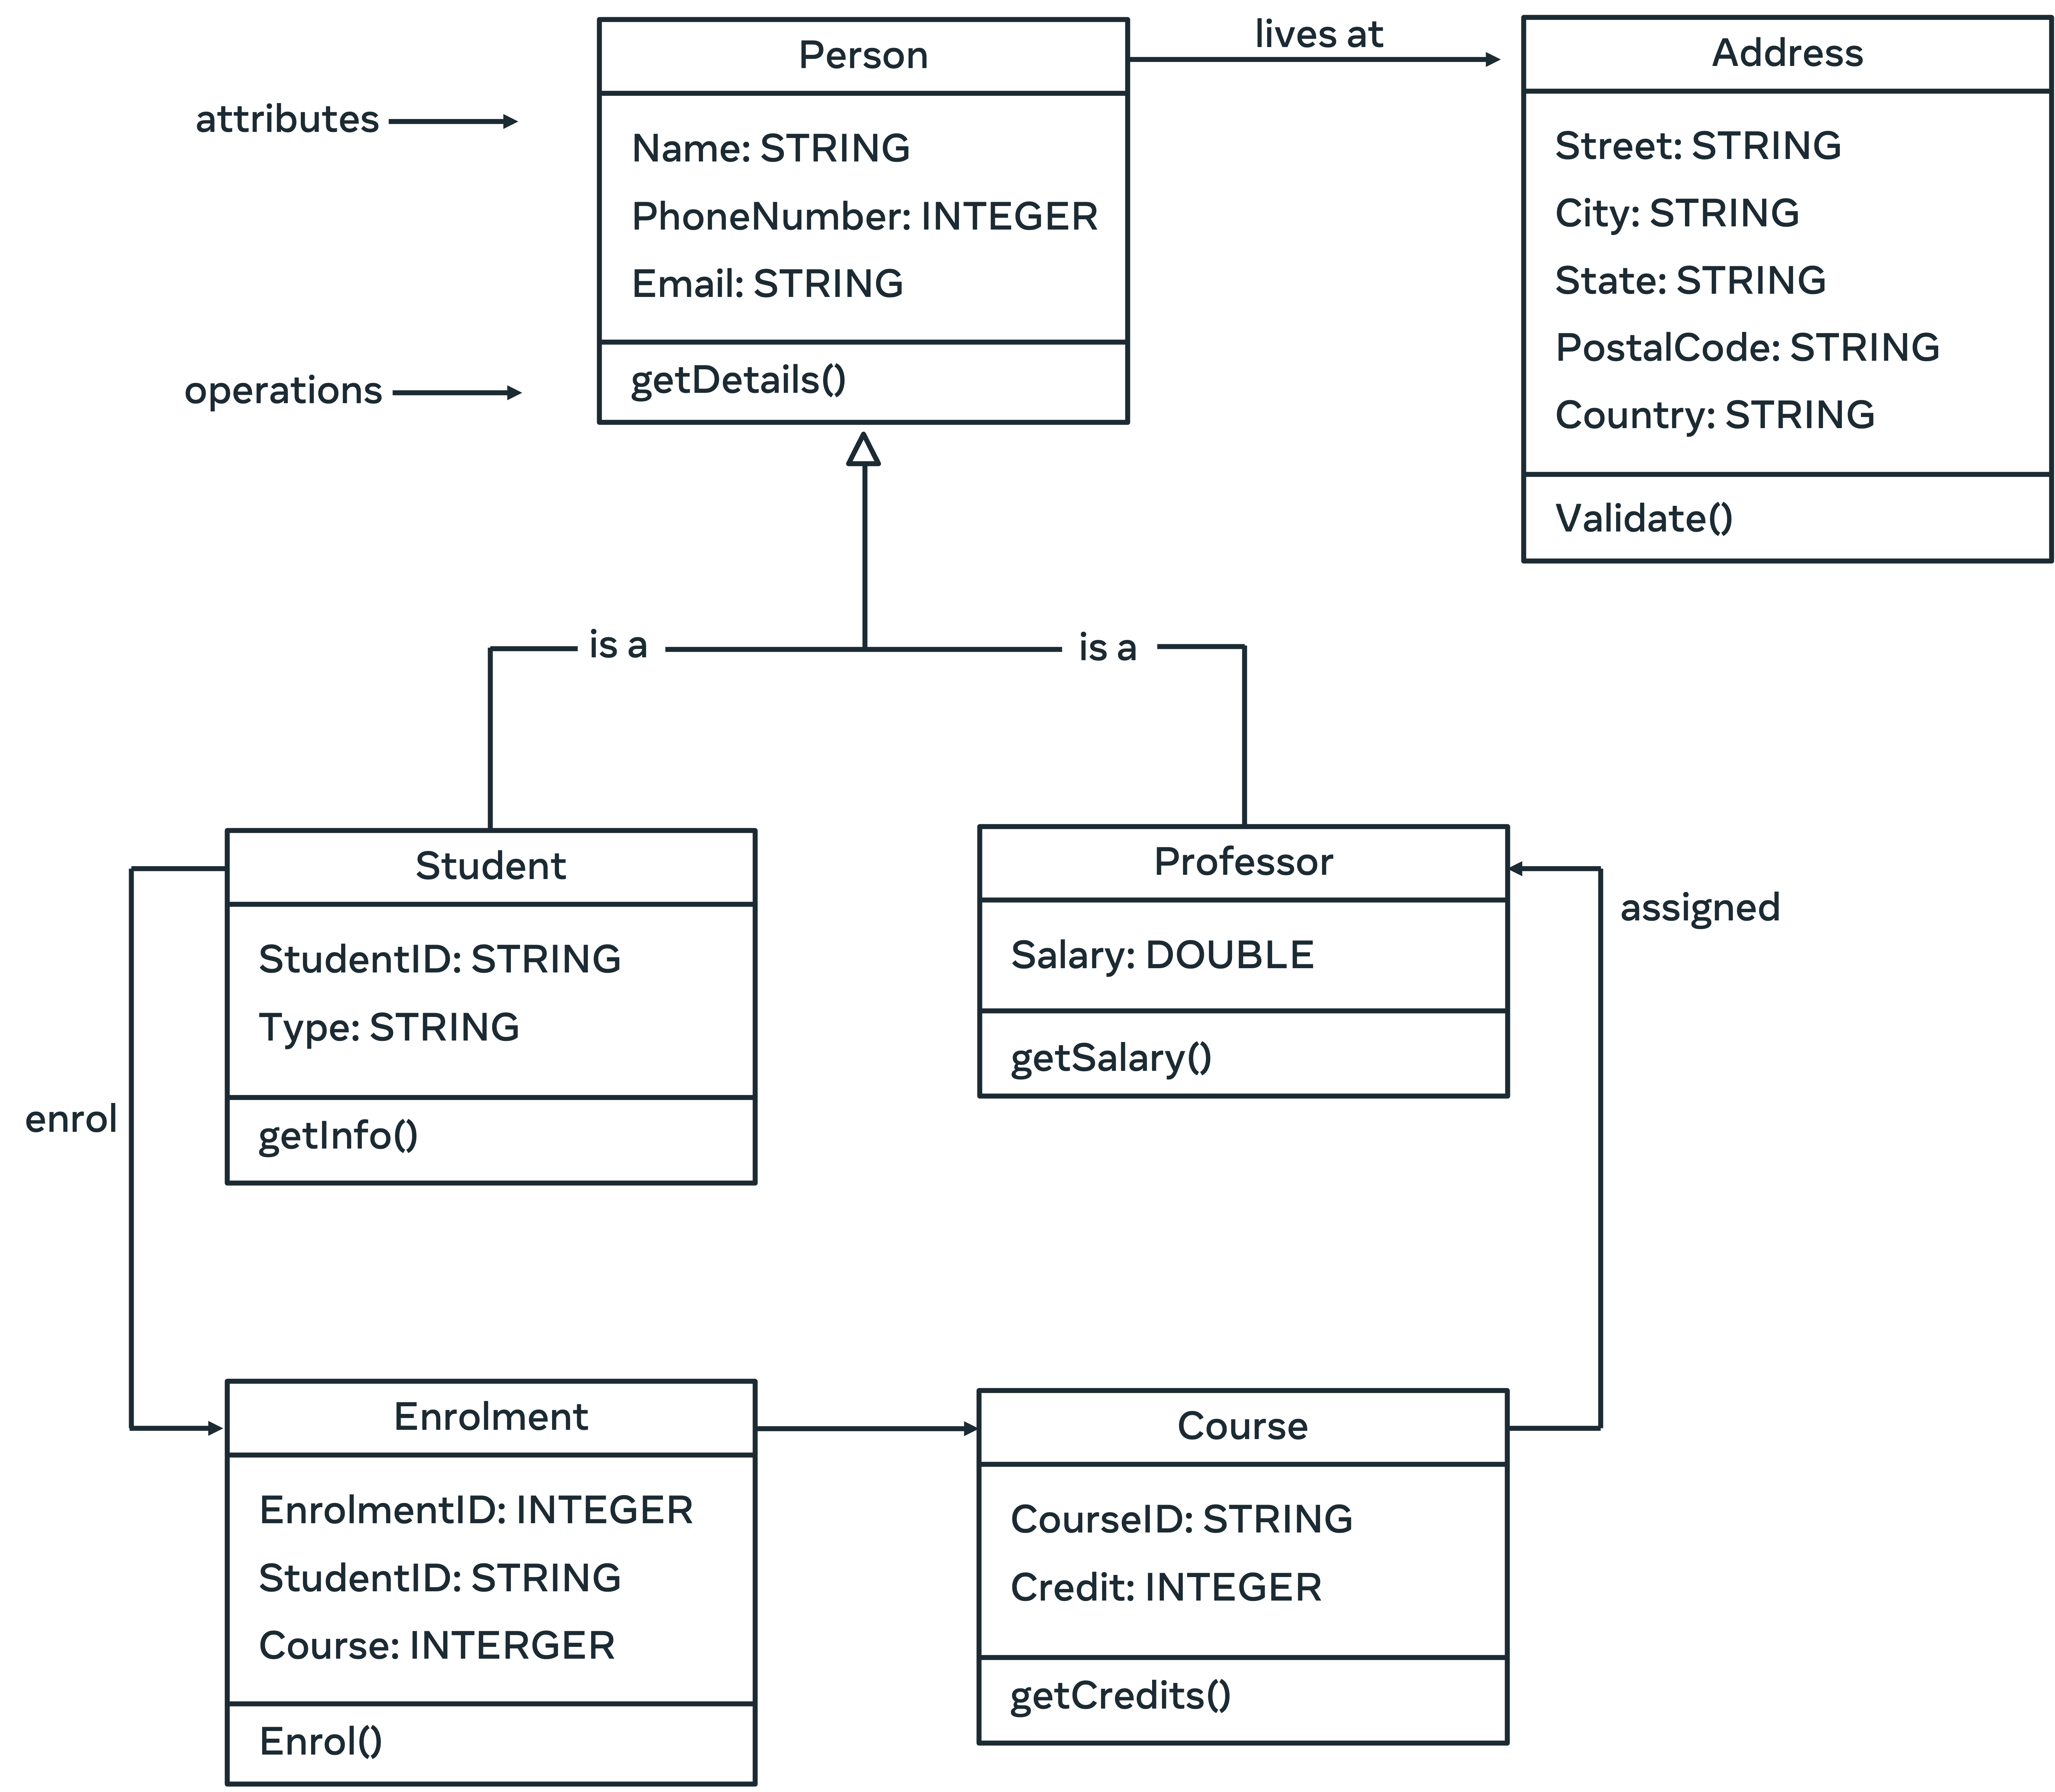
\includegraphics[width=0.8\textwidth]{./Picts/oo.png}
    \caption{}
\end{figure}

Dalam contoh ini, setiap kelas mewakili objek-objek serupa dalam basis data. Artinya, objek-objek serupa memiliki karakteristik dan perilaku yang sama. Misalnya, setiap mahasiswa yang terdaftar dalam sistem basis data memiliki kumpulan atribut (atau variabel instance) yang sama, seperti ID dan jenis. Selain itu, setiap instance objek dari suatu kelas menggunakan operasi yang sama yang dinyatakan dalam kelas tersebut.

Selain itu, terdapat berbagai jenis hubungan yang didefinisikan dalam diagram sebagai berikut:
\begin{itemize}
    \item Setiap siswa dan dosen adalah orang (hubungan pewarisan) dan setiap orang terkait dengan alamat.
    \item Setiap siswa dan dosen adalah subtipe dari orang, dan setiap orang berfungsi sebagai supertipe untuk setiap siswa dan dosen.
    \item Setiap pendaftaran melibatkan siswa dan mata kuliah. Kelas pendaftaran dalam hal ini disebut kelas asosiasi.
    \item Setiap dosen ditugaskan ke mata kuliah.
\end{itemize}

\subsubsection{Model Data Dimensional}
Model ini didasarkan pada dua konsep kunci, yaitu fakta (facts) dan dimensi (dimensions). Fakta adalah pengukuran yang diperoleh dari suatu proses, sedangkan dimensi mendefinisikan konteks pengukuran tersebut.

Keuntungan: Mengoptimalkan basis data untuk pengambilan data yang lebih cepat dan merestrukturisasi data untuk analisis yang lebih efisien.

\subsection{Pengantar Normalisasi Basis Data}
Normalisasi adalah proses yang digunakan untuk menyusun tabel dalam basis data agar mengurangi duplikasi data, menghindari implikasi modifikasi data, dan menyederhanakan kueri data.

Anomali yang umum terjadi dalam tabel basis data yang tidak dinormalisasi meliputi:
\begin{itemize}
    \item Insertion Anomaly: Ketika penambahan data baru memerlukan penambahan data tambahan.
    \item Update Anomaly: Ketika memperbarui satu kolom menyebabkan perlu memperbarui kolom lain di tabel.
    \item Deletion Anomaly: Ketika penghapusan satu data menyebabkan penghapusan data lain yang diperlukan.
\end{itemize}

\subsection{Tingkatan Normalisasi}
\subsubsection{First Normal Form(1NF)}
Menegakkan atomisitas data dan menghilangkan kelompok data yang berulang.

Contoh: Jika tabel produk \verb|M&G| menyimpan produk dalam satu sel, ini melanggar aturan atomisitas. Solusinya adalah membuat tabel produk dan tabel klien terpisah, masing-masing dengan kolom ID unik.

\subsubsection{Second Normal Form(2NF)}
Tabel harus sudah dalam 1NF dan tidak boleh memiliki ketergantungan fungsional atau parsial. Ini hanya terdapat jika primary keynya adalah Composite Primary Key

Contoh: Tabel status pengiriman \verb|M&G| memiliki kunci primer komposit (order ID dan product ID). Jika ada atribut non-kunci yang hanya bergantung pada satu bagian dari kunci komposit, seperti tanggal pesanan, maka harus dipindahkan ke tabel pesanan.

\subsubsection{Third Normal Form (3ND)}
menghilangkan duplikasi data yang tidak perlu dan memastikan konsistensi serta integritas data. Untuk sebuah tabel dapat memenuhi 3NF, tabel tersebut harus sudah memenuhi First Normal Form (1NF) dan Second Normal Form (2NF). Selain itu, 3NF juga mengatasi masalah ketergantungan transitif, di mana atribut non-kunci bergantung satu sama lain.

Contoh: Jika kota dan kode pos dalam tabel pesanan \verb|M&G| saling bergantung, maka harus dipisahkan menjadi dua tabel: satu untuk pesanan dan satu untuk kota, dengan kolom kode pos dan nama kota.

\subsection{Pengenalan MySQL Workbench}
\begin{itemize}
    \item MySQL Workbench adalah alat visual yang dikembangkan oleh Oracle untuk pemodelan dan manajemen basis data.
    \item Alat ini bersifat open source dan dapat digunakan di berbagai sistem operasi.
\end{itemize}

\subsubsection{Fitur Utama MySQL Workbench}
\begin{itemize}
    \item Visual SQL Editor: Memudahkan penulisan pernyataan SQL dengan fitur autocomplete dan highlighting.
    \item Migrasi Data: Memfasilitasi migrasi data antara versi MySQL yang berbeda dan sistem basis data relasional lainnya.
\end{itemize}

\subsubsection{Membuat Pengguna Baru}
\begin{itemize}
    \item MySQL Connection: Pilih koneksi MySQL untuk mengelola pengguna dan hak akses.
    \item Login menggunakan pengguna root dan pilih "Users and Privileges" untuk menambah pengguna baru.
    \item Tentukan nama pengguna, kata sandi, dan hak akses yang sesuai.
\end{itemize}

\subsubsection{Membuat Koneksi MySQL Baru}
\begin{itemize}
    \item Dari layar utama MySQL Workbench, pilih ikon plus untuk membuka formulir koneksi baru.
    \item Isi formulir dengan nama instance server, username, dan pastikan hostname adalah 127.0.0.1 dengan port 3306.
    \item Klik "Test Connection" untuk memastikan pengaturan koneksi berhasil.
\end{itemize}

\subsection{Data Management di MySQL Workbench}
\subsubsection{Membuat Skema Database}
Skema adalah struktur yang mendefinisikan cara data disimpan dalam database. Untuk membuat skema baru, pilih opsi "Create Schema" dan masukkan nama skema, misalnya \verb|mg_schema|.

Setelah membuat skema, Anda akan melihat skrip SQL yang dihasilkan, seperti \verb|CREATE SCHEMA 'mg_schema'|. Klik "Apply" untuk menerapkannya.

\subsubsection{Membuat Tabel}
Tabel adalah struktur yang menyimpan data dalam baris dan kolom. Untuk membuat tabel baru, pilih "Create Table" dan masukkan nama tabel, misalnya staff.

Kolom adalah elemen dalam tabel yang menyimpan data. Misalnya, kolom StaffID dengan tipe data integer dan ditetapkan sebagai primary key. Kolom lain termasuk FullName, ContactNumber, Role, dan Email.

\subsubsection{Mengelola Data}
Insert Statement digunakan untuk menambahkan data ke tabel. Anda dapat mengisi data langsung di grid tabel dan menggunakan MySQL Workbench untuk menghasilkan pernyataan insert otomatis.

Query adalah proses untuk mengambil data dari database. Anda dapat menggunakan SQL Editor untuk menulis query, seperti \verb|SELECT * FROM staff_view| untuk menampilkan semua data dari tabel \verb|staff_view|.

\subsubsection{Membuat View}
View adalah tabel virtual yang menyajikan data dari satu atau lebih tabel. Untuk membuat view, gunakan pernyataan SQL CREATE VIEW dan tambahkan alias untuk kolom agar lebih mudah dibaca.

\subsubsection{Sintaks Penting}
\begin{itemize}
    \item \verb|CREATE SCHEMA 'mg_schema'|: Membuat skema baru.
    \item \verb|CREATE TABLE staff (...)|: Membuat tabel baru dengan kolom yang ditentukan.
    \item \verb|INSERT INTO staff (...) VALUES (...)|: Menambahkan data ke tabel.
    \item \verb|SELECT * FROM staff_view|: Mengambil semua data dari view.
\end{itemize}

\subsection{Database Modeling di MySQL Workbench}
\subsubsection{Membuat Model Database}
\begin{itemize}
    \item MySQL Workbench: Alat untuk merancang dan mengelola database. Anda dapat membuat model database untuk menyimpan informasi tentang pelanggan dan pesanan.
    \item Forward Engineering: Proses mengubah model data menjadi skema SQL yang dapat diimplementasikan secara otomatis ke dalam MySQL.
\end{itemize}

\subsubsection{Langkah-langkah Membuat Model}
\begin{itemize}
    \item Membuat Skema: Klik "model's view" dan buat skema baru, misalnya \verb|mangata_gallo|.
    \item Diagram Data Model: Buat diagram ER (Entity-Relationship) dengan menambahkan tabel.
\end{itemize}

\subsubsection{Menambahkan Tabel dan Kolom}
\begin{itemize}
    \item Menambahkan Tabel: Klik ikon "Add Table" untuk membuat entitas tabel.
    \item Menambahkan Kolom: Ganti nama kolom default dan atur tipe data serta atribut seperti \verb|NOT NULL dan AUTO_INCREMENT|.
\end{itemize}

\subsubsection{Mengatur Foreign Key}
Foreign Key: Kolom yang menghubungkan tabel satu dengan yang lain. Misalnya, \verb|customer_id_fk| yang merujuk ke customer ID di tabel pelanggan.

\subsubsection{Menyimpan dan Mengimplementasikan Model}
\begin{itemize}
    \item Menyimpan Model: Klik "File Save As" untuk menyimpan model dengan nama yang diinginkan.
    \item Menyinkronkan ke MySQL: Gunakan fitur forward engineer untuk menghubungkan ke server MySQL dan menerapkan skema yang telah dibuat.
\end{itemize}

\subsubsection{Reverse Engineering}
Reverse Engineering: Proses membangun diagram ER dari database yang sudah ada.

Langkah-langkah: Pilih opsi reverse engineer dari menu database, pilih skema yang ingin diambil, dan eksekusi untuk mendapatkan diagram ER baru.

\subsection{MySQL Workbench untuk Data Modeling dan Data Management}
\subsubsection{Overview}
MySQL Workbench (WB) adalah alat visual terpadu untuk pemodelan basis data dan pengelolaan basis data. WB dikembangkan oleh Oracle, perusahaan yang mengelola MySQL. MySQL Workbench adalah alat gratis, sumber terbuka, dan lintas platform yang dapat dijalankan di Windows, Mac, dan Linux.

MySQL Workbench memungkinkan Anda mempercepat proses desain basis data dengan menggunakan editor SQL visual. Alat ini juga memungkinkan Anda memigrasikan data dari berbagai sistem basis data relasional.

\subsubsection{Visual Database Design}
MySQL Workbench memudahkan desain dan pemeliharaan basis data. Alat ini memungkinkan insinyur basis data untuk mendokumentasikan persyaratan dalam bentuk diagram ER yang visual. Hal ini memungkinkan Anda untuk berkomunikasi ide desain Anda dengan pemangku kepentingan secara profesional.

Alat desain MySQL WB memfasilitasi pengembangan basis data berbasis model, yang mengotomatiskan proses pengembangan tanpa perlu mengkodekan setiap bagian sistem basis data.

Selain itu, dengan menggunakan MySQL WB, insinyur basis data harus merancang model data yang memenuhi standar yang diharapkan, jika tidak, mereka tidak dapat mengimplementasikan model data tersebut secara langsung di MySQL.

Dengan kata lain, MySQL WB memungkinkan Anda mengembangkan diagram entitas-hubungan yang lengkap dengan tata letak otomatis dan pengaturan model data.

\subsubsection{Forward and Reverse Engineer Methods}
MySQL Workbench menyediakan fitur untuk membuat model data dalam desainer visual. Anda dapat menggunakan metode \textbf{Forward Engineer} untuk membuat model data yang relevan di server MySQL Anda. Skema SQL akan dihasilkan secara otomatis untuk Anda. Anda dapat mengedit kode jika diperlukan, atau menjalankannya dengan beberapa klik mouse.

MySQL Workbench juga menawarkan metode \textbf{Reverse Engineer}. Anda dapat menggunakan metode ini untuk membuat atau mengimpor berkas basis data MySQL, lalu menghasilkan model data yang relevan dari skrip SQL. Anda dapat memodifikasi model jika diperlukan, dan kemudian menggunakan metode Forward Engineer untuk membuat sistem basis data baru di MySQL.

\subsubsection{Database Management}
Pengelolaan database umumnya melibatkan pemeliharaan berbagai versi skema database Anda. Untuk membantu Anda dalam pengelolaan database, MySQL WB dapat digunakan untuk melakukan fungsi Sinkronisasi dan Perbandingan Skema. Fitur-fitur ini memungkinkan Anda untuk membandingkan dua database atau sebuah database dengan model data, sehingga Anda dapat secara visual mendeteksi perbedaan di antara keduanya. MySQL WB juga memungkinkan Anda untuk menyinkronkan model data dengan database yang aktif dan sebaliknya.

\subsubsection{Database Documentation}
Sebagai seorang insinyur basis data, Anda perlu mendokumentasikan desain basis data Anda. Hal ini dapat memakan waktu yang cukup lama. MySQL Workbench menyediakan alat dokumentasi bernama DBDoc untuk mendokumentasikan semua detail desain basis data Anda. Anda dapat menggunakan alat ini untuk menghasilkan dokumentasi model basis data Anda dalam format HTML atau teks biasa.

\subsubsection{Visual SQL Editor}
MySQL WB visual SQL editor digunakan untuk menulis, menjalankan, dan mendebug pernyataan SQL. Alat ini juga memudahkan penyelesaian kode SQL dan menyediakan daftar kata kunci dan objek SQL yang sensitif terhadap konteks.

Selain itu, editor ini dilengkapi dengan pemformat kode SQL yang secara otomatis memformat kode SQL agar lebih mudah dibaca dan diedit. Fitur berguna lainnya meliputi:
\begin{itemize}
    \item Penyorotan sintaksis SQL,
    \item Pembangkitan kode SQL,
    \item Kemampuan untuk menggunakan kembali potongan kode SQL favorit Anda,
    \item Riwayat eksekusi semua kueri SQL yang dijalankan,
\end{itemize}

Dan kemampuan untuk dengan cepat membuat tabel, indeks, tampilan, prosedur tersimpan, pemicu, dan fungsi.

\subsubsection{Visual Database Administration}
Dengan MySQL WB, Anda memiliki kendali administratif penuh atas semua aspek server MySQL Anda, termasuk:
\begin{itemize}
    \item Akun pengguna,
    \item Peran,
    \item Hak akses,
    \item Mulai/henti server,
    \item Log,
    \item Dan konfigurasi server.
\end{itemize}

\subsubsection{Data Management}
MySQL WB menyediakan fitur-fitur berguna untuk mengelola data dalam basis data MySQL, termasuk kemampuan untuk mengimpor dan mengekspor berkas mysqldump, serta mengekspor hasil kueri sebagai berkas CSV, XML, dan HTML.

WB Visual Data Editor juga memungkinkan Anda untuk melihat dan mengedit hasil kueri dalam tabel grid.

Anda juga dapat melihat beberapa hasil kueri dalam jendela data visual yang sama. Dan Anda dapat melakukan pencarian data dan pencarian pola di seluruh tabel dan skema.

\subsubsection{Data Migration}
Di MySQL WB, Anda dapat menggunakan Database Migration Wizard untuk melakukan migrasi data antara versi yang berbeda dari server MySQL.

Selain itu, Anda juga dapat melakukan migrasi data dengan sistem manajemen basis data relasional lainnya seperti Microsoft SQL Server, Sybase ASE, Sybase SQL Anywhere, PostgreSQL, dan SQLite.





\newpage

\section{Data Warehousing}
\subsection{Apa itu Data Warehouse?}
Data Warehouse adalah repositori data terpusat yang mengumpulkan, menyimpan, dan memproses data dari berbagai sumber. Ini memisahkan beban kerja analisis data dari beban kerja transaksi standar dari sistem manajemen basis data biasa.

Pengguna dapat melakukan query pada data ini untuk melakukan analisis data. Tipe basis data ini dikenal sebagai Online \textbf{Analytical Processing (OLAP)}.

\subsection{Karakteristik Utama Data Warehouse}
\subsubsection{Subject-Oriented}
Data warehouse dibangun dengan fokus pada satu atau lebih area subjek. Misalnya, global superstore dapat membangun data warehouse yang fokus pada penjualan untuk menemukan informasi terkait proses penjualan mereka.

\subsubsection{Integrated}
Data warehouse mengintegrasikan data dari berbagai sumber dalam format yang konsisten. Ini juga menyelesaikan masalah seperti konflik penamaan dan tipe data. Contohnya, data dari pembelian online, interaksi website, dan media sosial diintegrasikan.

\subsubsection{Non-Volatile}
Data yang dimuat ke dalam data warehouse tidak boleh dihapus. Tujuan dari data warehouse adalah untuk menganalisis data sebagaimana adanya, sehingga semakin banyak data yang ada, semakin baik hasil analisisnya.

\subsubsection{time-Variant}
Data warehouse mengumpulkan data selama periode yang panjang untuk mengukur perubahan data dari waktu ke waktu. Ini membantu pengguna menemukan tren, pola, dan hubungan antara elemen data.

\subsection{Jenis Data dalam Data Warehouse}
\subsubsection{Structured Data}
Data yang disajikan dalam format terstruktur dalam model data yang terdefinisi dengan baik, seperti model basis data relasional.

\subsubsection{Semi-Structured Data}
Data yang hanya sebagian terstruktur dan memerlukan lebih banyak usaha untuk analisis. Contohnya adalah email yang memiliki data terstruktur seperti pengirim dan subjek, tetapi isi emailnya tidak terstruktur.

\subsubsection{Unstructured Data}
Data yang tidak mengikuti model data yang terdefinisi. Ini bisa mencakup teks, video, atau audio. Menganalisis data tidak terstruktur memerlukan mekanisme analitik data yang lebih canggih seperti machine learning dan data mining.

\subsection{Komponen Arsitektur Data Warehouse}
\begin{figure}[H]
    \centering
    
\includegraphics[width=0.8\textwidth]{./Picts/ss1.png}
    \caption{}
\end{figure}

Sumber Data:
\begin{itemize}
    \item Sumber data eksternal seperti Global Super Store, survei online, atau data media sosial.
    \item Sumber data internal dari database perusahaan mengenai pelanggan dan produk, serta data operasional dari aktivitas bisnis sehari-hari.
\end{itemize}
Data Staging:
\begin{itemize}
    \item Area staging data mencakup proses ETL (Extract, Transform, Load) yang digunakan untuk mengekstrak data dari sumber, mengubahnya ke format yang konsisten, dan memuatnya ke dalam data warehouse.
\end{itemize}

\subsection{Penyimpanan dan Metadata}
Data Storage merupakan repositori database pusat yang menyimpan data dalam format relasional. Ini juga mencakup metadata yang berisi informasi tentang data, seperti asal data dan atribut tabel.

Metadata adalah "daftar isi" untuk data dalam data warehouse, membantu insinyur database mengelola dan melacak perubahan dalam sistem sumber mereka.

\subsection{Data Marts dan Analisis Data}
Data Marts adalah basis data yang berfokus pada subjek tertentu untuk memenuhi kebutuhan kelompok pengguna tertentu, seperti departemen dalam organisasi.

Data Analytics: Proses analisis data menggunakan teknik seperti data mining untuk menghasilkan laporan yang memberikan informasi penting tentang penjualan, keuntungan, dan aspek lainnya dari bisnis.

\subsection{Praktik Terbaik terkait Data Warehousing}
\begin{itemize}
    \item Pisahkan operasi analitis dan transaksional.
    \item Gunakan solusi yang dapat diskalakan untuk memproses data yang semakin besar.
    \item Bangun arsitektur yang fleksibel dan mudah dipahami, serta dokumentasikan pengembangan data warehouse.
\end{itemize}

\subsection{Pendalaman Data Warehouse ETL Process}
\subsubsection{Overview}
ETL adalah singkatan dari "Extract, Transform, and Load". Ini merupakan bagian penting dari fase penyiapan data dalam arsitektur data warehouse. ETL menggambarkan serangkaian proses yang mengekstrak data dari sistem sumber yang berbeda, mengubah data menjadi format yang sesuai, dan memuatnya ke dalam repositori data warehouse untuk analisis data.

Secara umum, data warehousing melibatkan proses ETL yang kompleks dan memerlukan keterlibatan aktif dari pemangku kepentingan, termasuk insinyur data, analis data, analis bisnis, penguji, dan manajer.

Sebagai insinyur database, Anda harus mengevaluasi dengan cermat setiap perubahan yang berdampak pada bisnis dalam desain proses ETL di data warehouse. Anda harus memastikan pemisahan yang lengkap antara operasi analitik dan operasi transaksional sehari-hari. Anda juga memerlukan solusi yang skalabel untuk memproses jumlah data yang sangat besar.

\subsubsection{Bagaimana ETL Bekerja}
Proses ETL tiga langkah mewakili alur kerja yang memindahkan data dari berbagai sumbernya dan mengintegrasikannya ke dalam data warehouse. Ada tiga langkah dalam proses ini:
\begin{itemize}
    \item Ekstraksi data.
    \item Transformasi.
    \item Dan pemuatan.
\end{itemize}

\subsubsection{Step 1: Data Extraction}
Langkah ini dalam proses melibatkan pengambilan data dari berbagai sumber ke area penyimpanan sementara. Misalnya, Global Super Store mungkin menggunakan sistem manajemen basis data dan file yang berbeda untuk mengelola data mereka di departemen logistik, operasional, penjualan, dan pemasaran. Hal ini dapat mencakup MySQL, Oracle, PostgreSQL, lembar Excel, dan file teks biasa, seperti yang ditunjukkan dalam diagram berikut.

\begin{figure}[H]
    \centering
    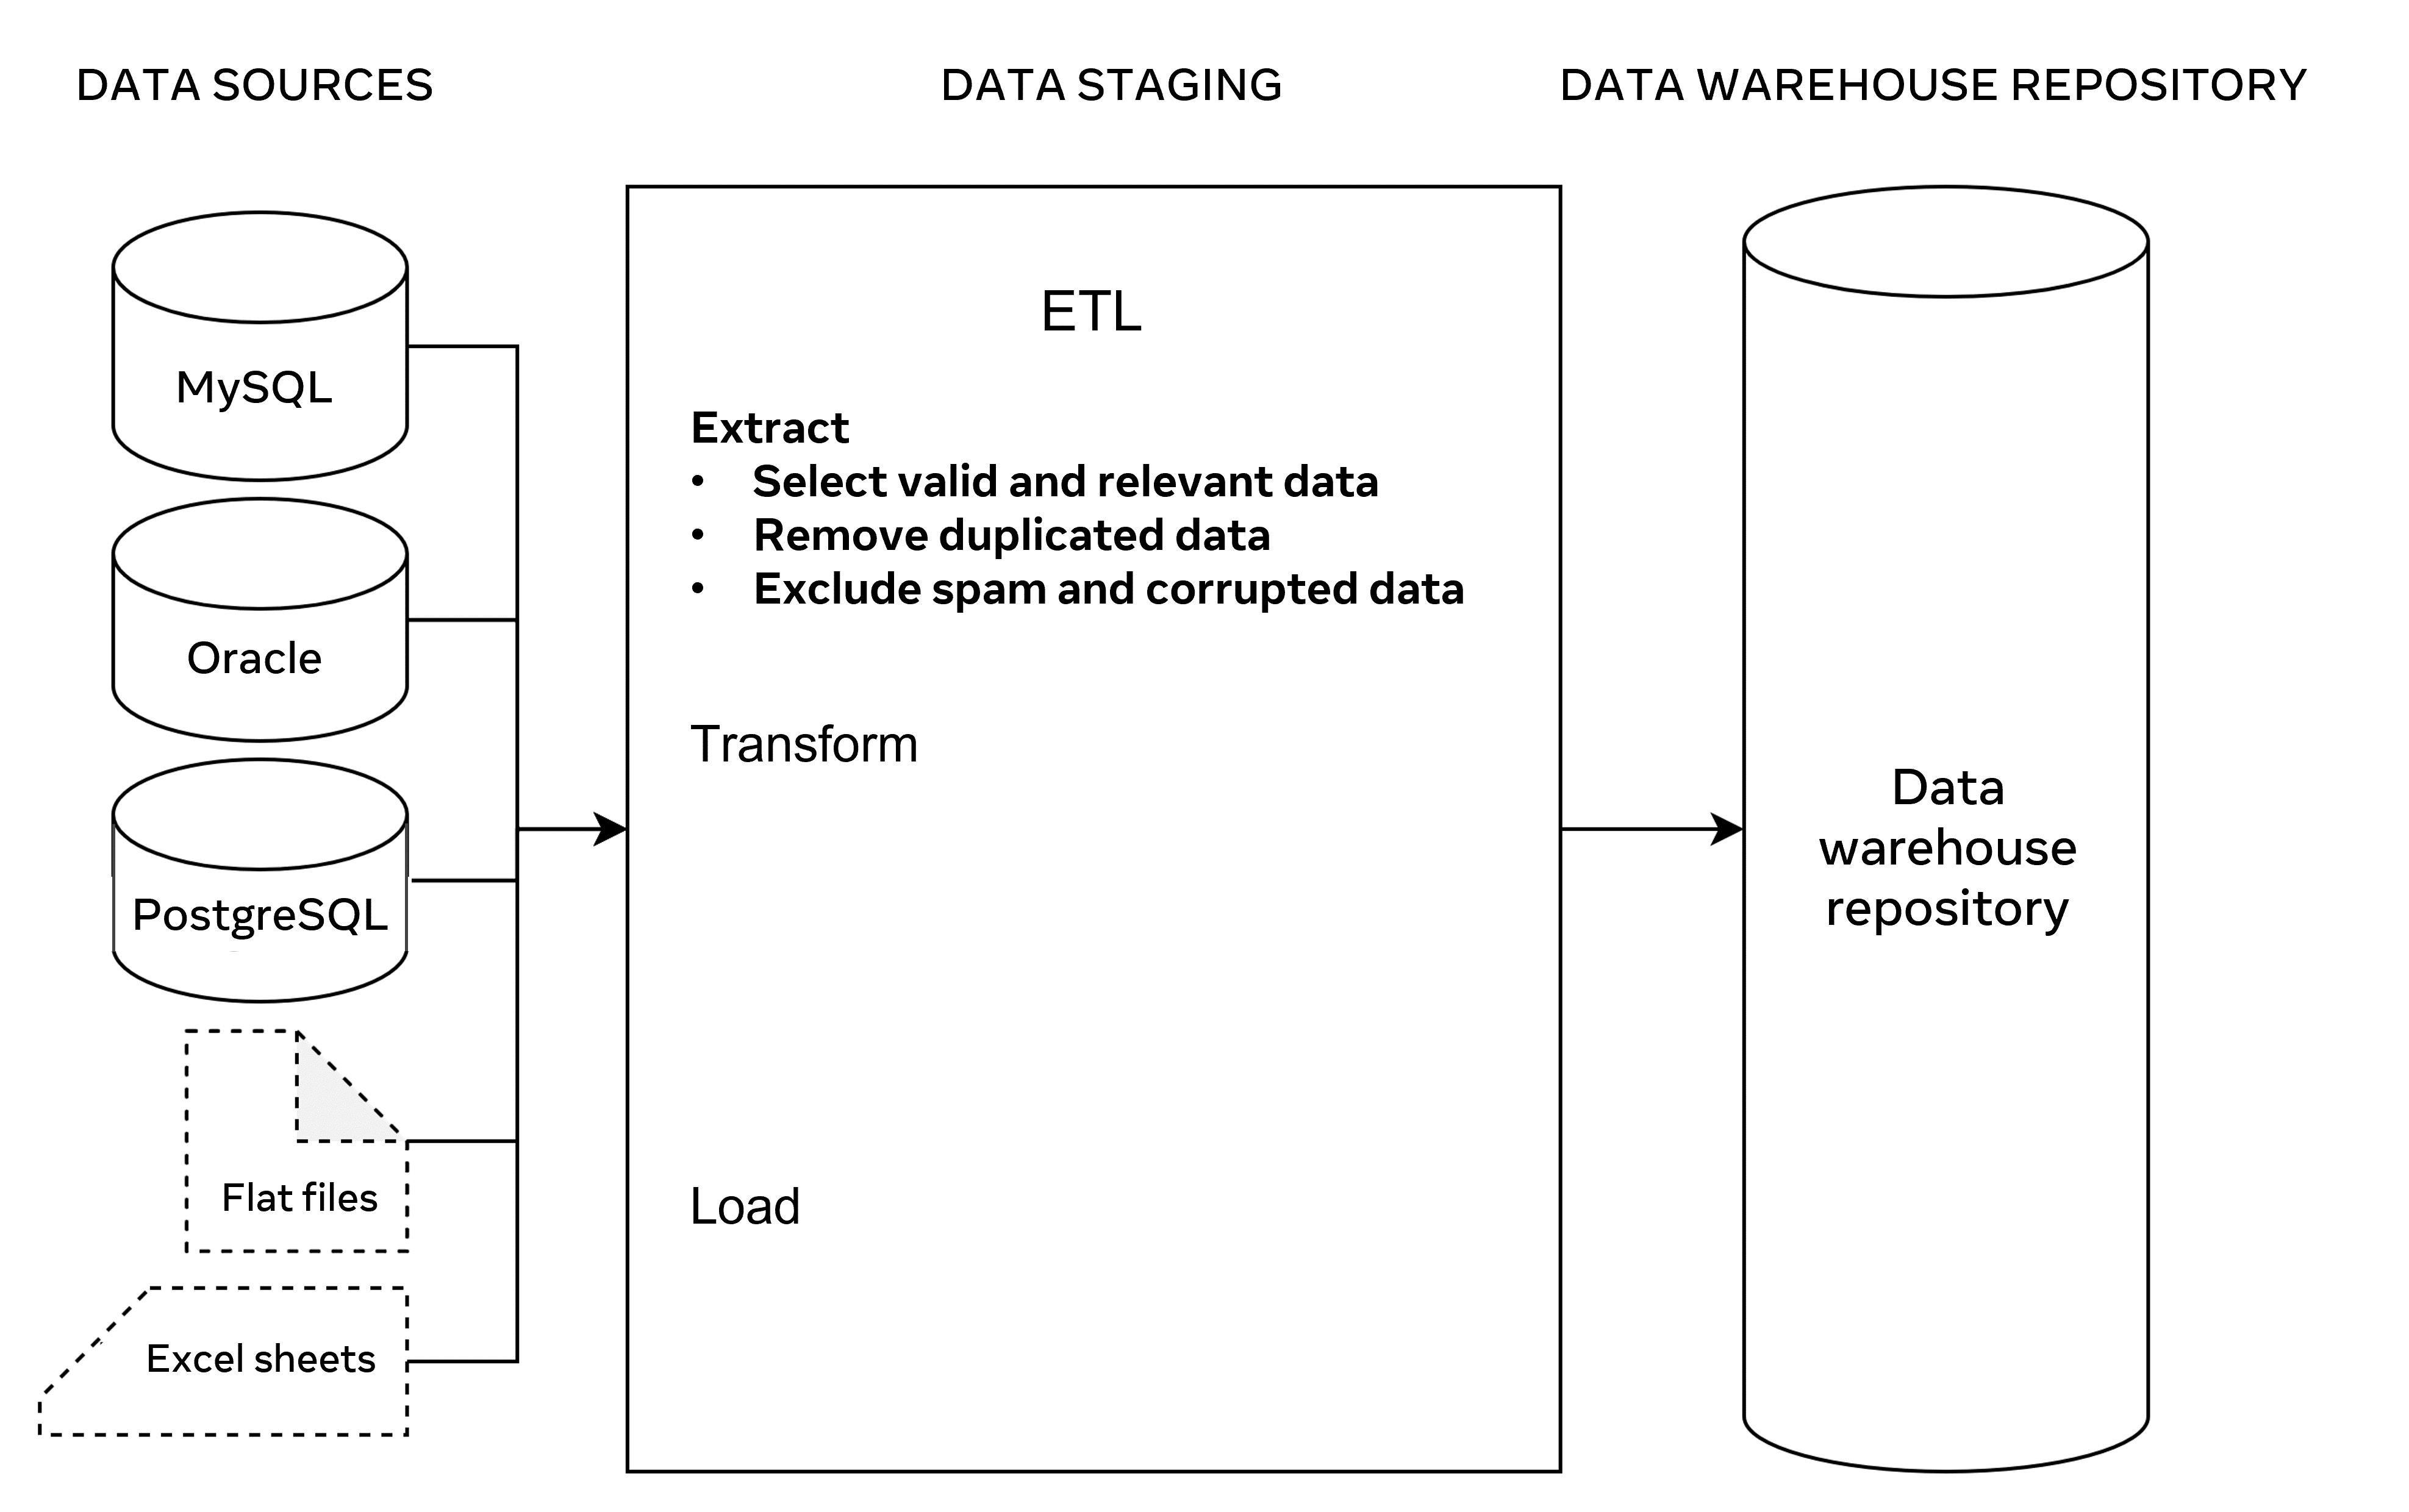
\includegraphics[width=0.8\textwidth]{./Picts/etls1.png}
    \caption{}
\end{figure}

Global Super Store mengekstrak data dari masing-masing sumber ini di area penyiapan. Saat merancang proses ini, penting bagi Anda untuk:
\begin{itemize}
    \item Hanya mengekstrak data yang relevan untuk menghindari kelebihan data.
    \item Menyertakan data yang valid dan menghapus semua duplikasi untuk mendapatkan hasil yang lebih akurat.
    \item Mengecualikan data spam dan data yang rusak, karena hal ini akan menghemat banyak waktu selama proses pembersihan dan persiapan data.
    \item Memvalidasi data dengan data asli di sumber untuk memastikan data dapat digunakan dengan cara yang sama di data warehouse.
\end{itemize}

\subsubsection{Step 2: Transformation}
Proses ini memerlukan konversi data dari satu format ke format lain, atau dari satu struktur ke struktur lain sesuai dengan model data yang telah ditetapkan di data warehouse. Langkah ini sangat penting untuk mengintegrasikan data ke dalam repositori data warehouse.

Data yang sudah terintegrasi dalam basis data relasional mungkin tidak memerlukan transformasi. Data tersebut dapat diimpor langsung ke repositori data warehouse tanpa perubahan. Namun, Anda mungkin perlu membersihkan dan mempersiapkan data sebelum menggunakannya untuk analisis data.

Misalnya, jika nilai nama depan dan nama belakang pelanggan disimpan terpisah dalam dua kolom yang berbeda, maka keduanya dapat digabungkan ke dalam kolom 'nama lengkap' sebelum dimuat ke repositori data warehouse. Atau jika data mencakup biaya pembelian dan penjualan, maka Anda dapat membuat kolom baru yang dihitung untuk keuntungan data.

Transformasi data menjadi lebih penting ketika Anda bekerja dengan data mentah (seperti jenis data atomik yang tidak dapat diolah menjadi informasi berguna oleh komputer secara mandiri). Contoh data mentah yang baik meliputi log komputer, cookie navigasi pengguna, dan riwayat pencarian. Jenis data ini dapat ditemukan dalam file teks biasa atau file nilai yang dipisahkan koma (CSV).

Dalam data warehouse, Anda harus menyertakan data terstruktur untuk analisis data. Untuk melakukannya, Anda harus mengorganisir data yang telah diubah dalam tabel, mendefinisikan data dengan tipe data spesifik, dan menetapkan batasan dalam tabel dan kolom. Hal ini menciptakan catatan data terkait yang dapat diakses, diinterogasi, dan dianalisis untuk menyajikan informasi yang berguna.

Tugas utama dalam proses transformasi meliputi pemformatan, pembersihan, persiapan, pengorganisasian, dan integrasi data, seperti yang ditunjukkan dalam diagram berikut.

\begin{figure}[H]
    \centering
    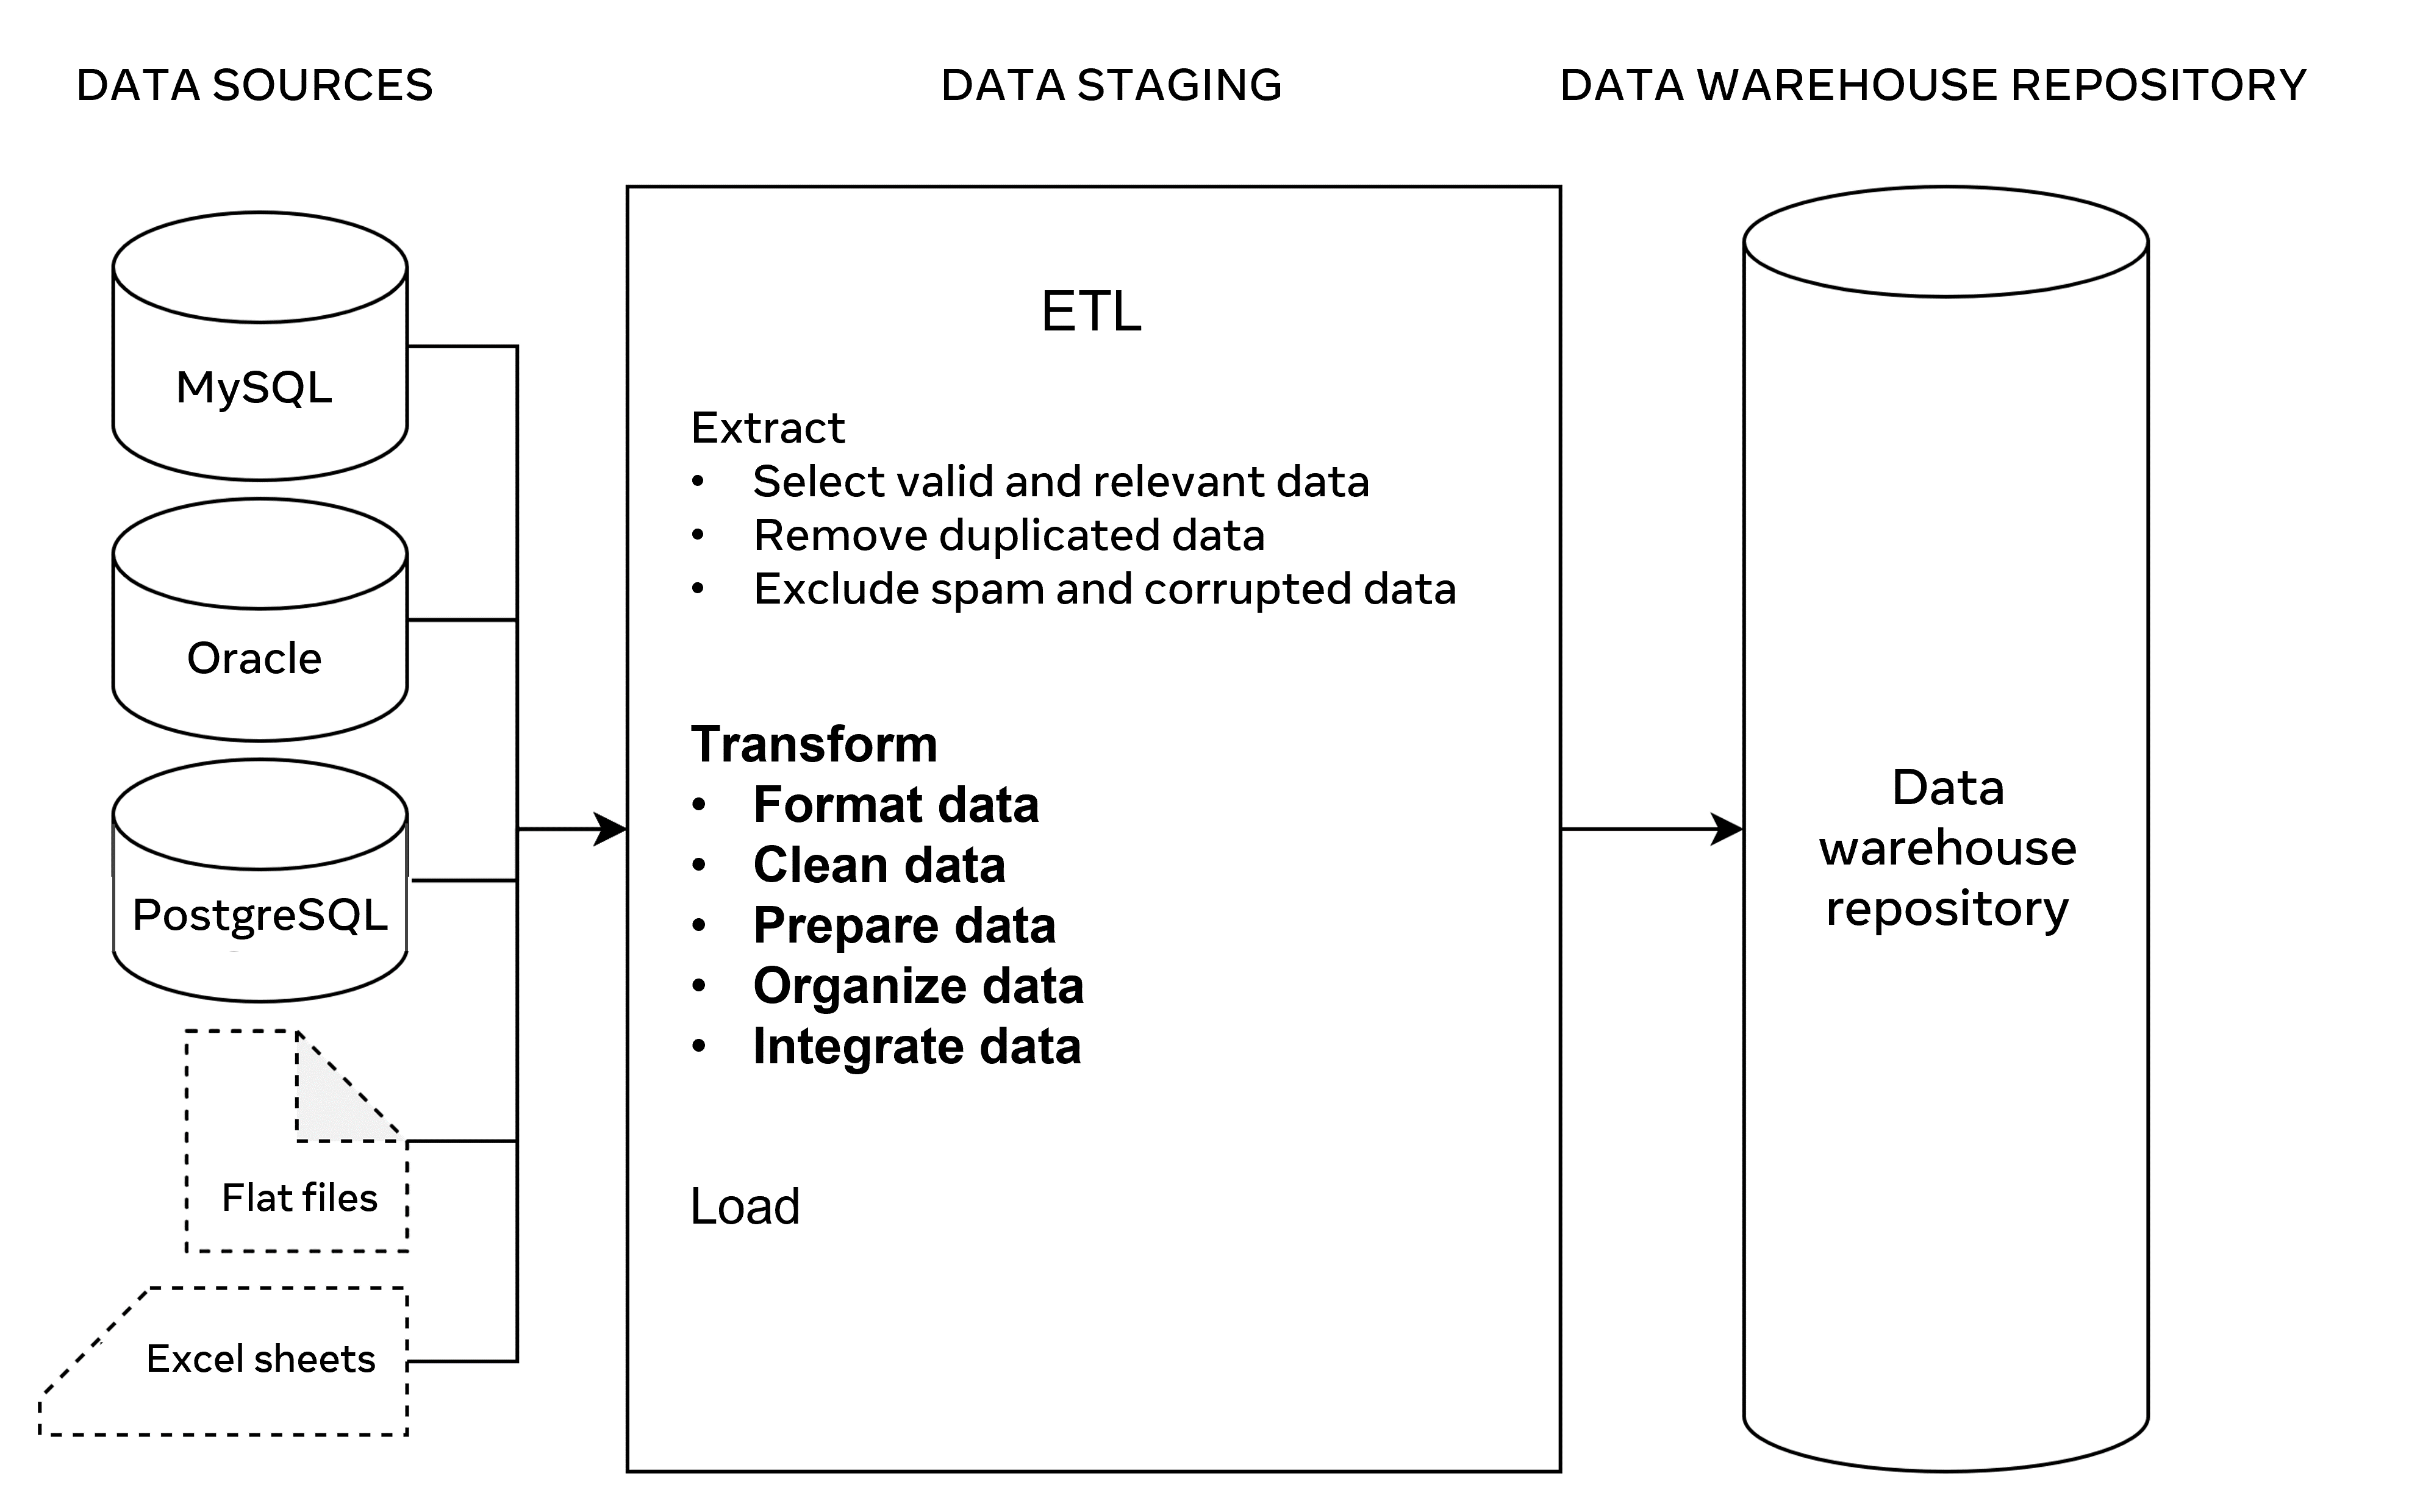
\includegraphics[width=0.8\textwidth]{./Picts/etls2.png}
    \caption{}
\end{figure}

Penting juga untuk memastikan integritas dan konsistensi data pada fase Transformasi. Misalnya, nama pelanggan mungkin ditulis dengan cara yang berbeda di berbagai sumber data, seperti John atau Jon. Atau nomor telepon dapat dicatat dengan cara yang berbeda (misalnya, dengan atau tanpa kode negara). Tanggal dan waktu juga dapat dikumpulkan dalam format yang berbeda.

\subsubsection{Step 3: Loading}
Proses ini merupakan langkah terakhir dalam ETL. Pada langkah ini, sejumlah besar data dimuat ke dalam repositori data warehouse. Oleh karena itu, penting untuk menerapkan mekanisme pemulihan jika terjadi kegagalan pemuatan data. Hal ini berarti Anda dapat melanjutkan proses pemuatan dari titik kegagalan tanpa kehilangan data dan sambil tetap menjaga integritas data.

Dalam konteks ini, Anda dapat melakukan tiga jenis pemuatan data:
\begin{itemize}
    \item Pemuatan awal: Memuat data yang diekstraksi ke repositori data warehouse.
    \item Pemuatan incremental: Memuat data baru dari sumber data ke repositori saat ini.
    \item Pemuatan refresh penuh: Menghapus isi database di repositori data warehouse secara sebagian atau seluruhnya dan memuatnya kembali dengan data baru yang segar.
\end{itemize}

\begin{figure}[H]
    \centering
    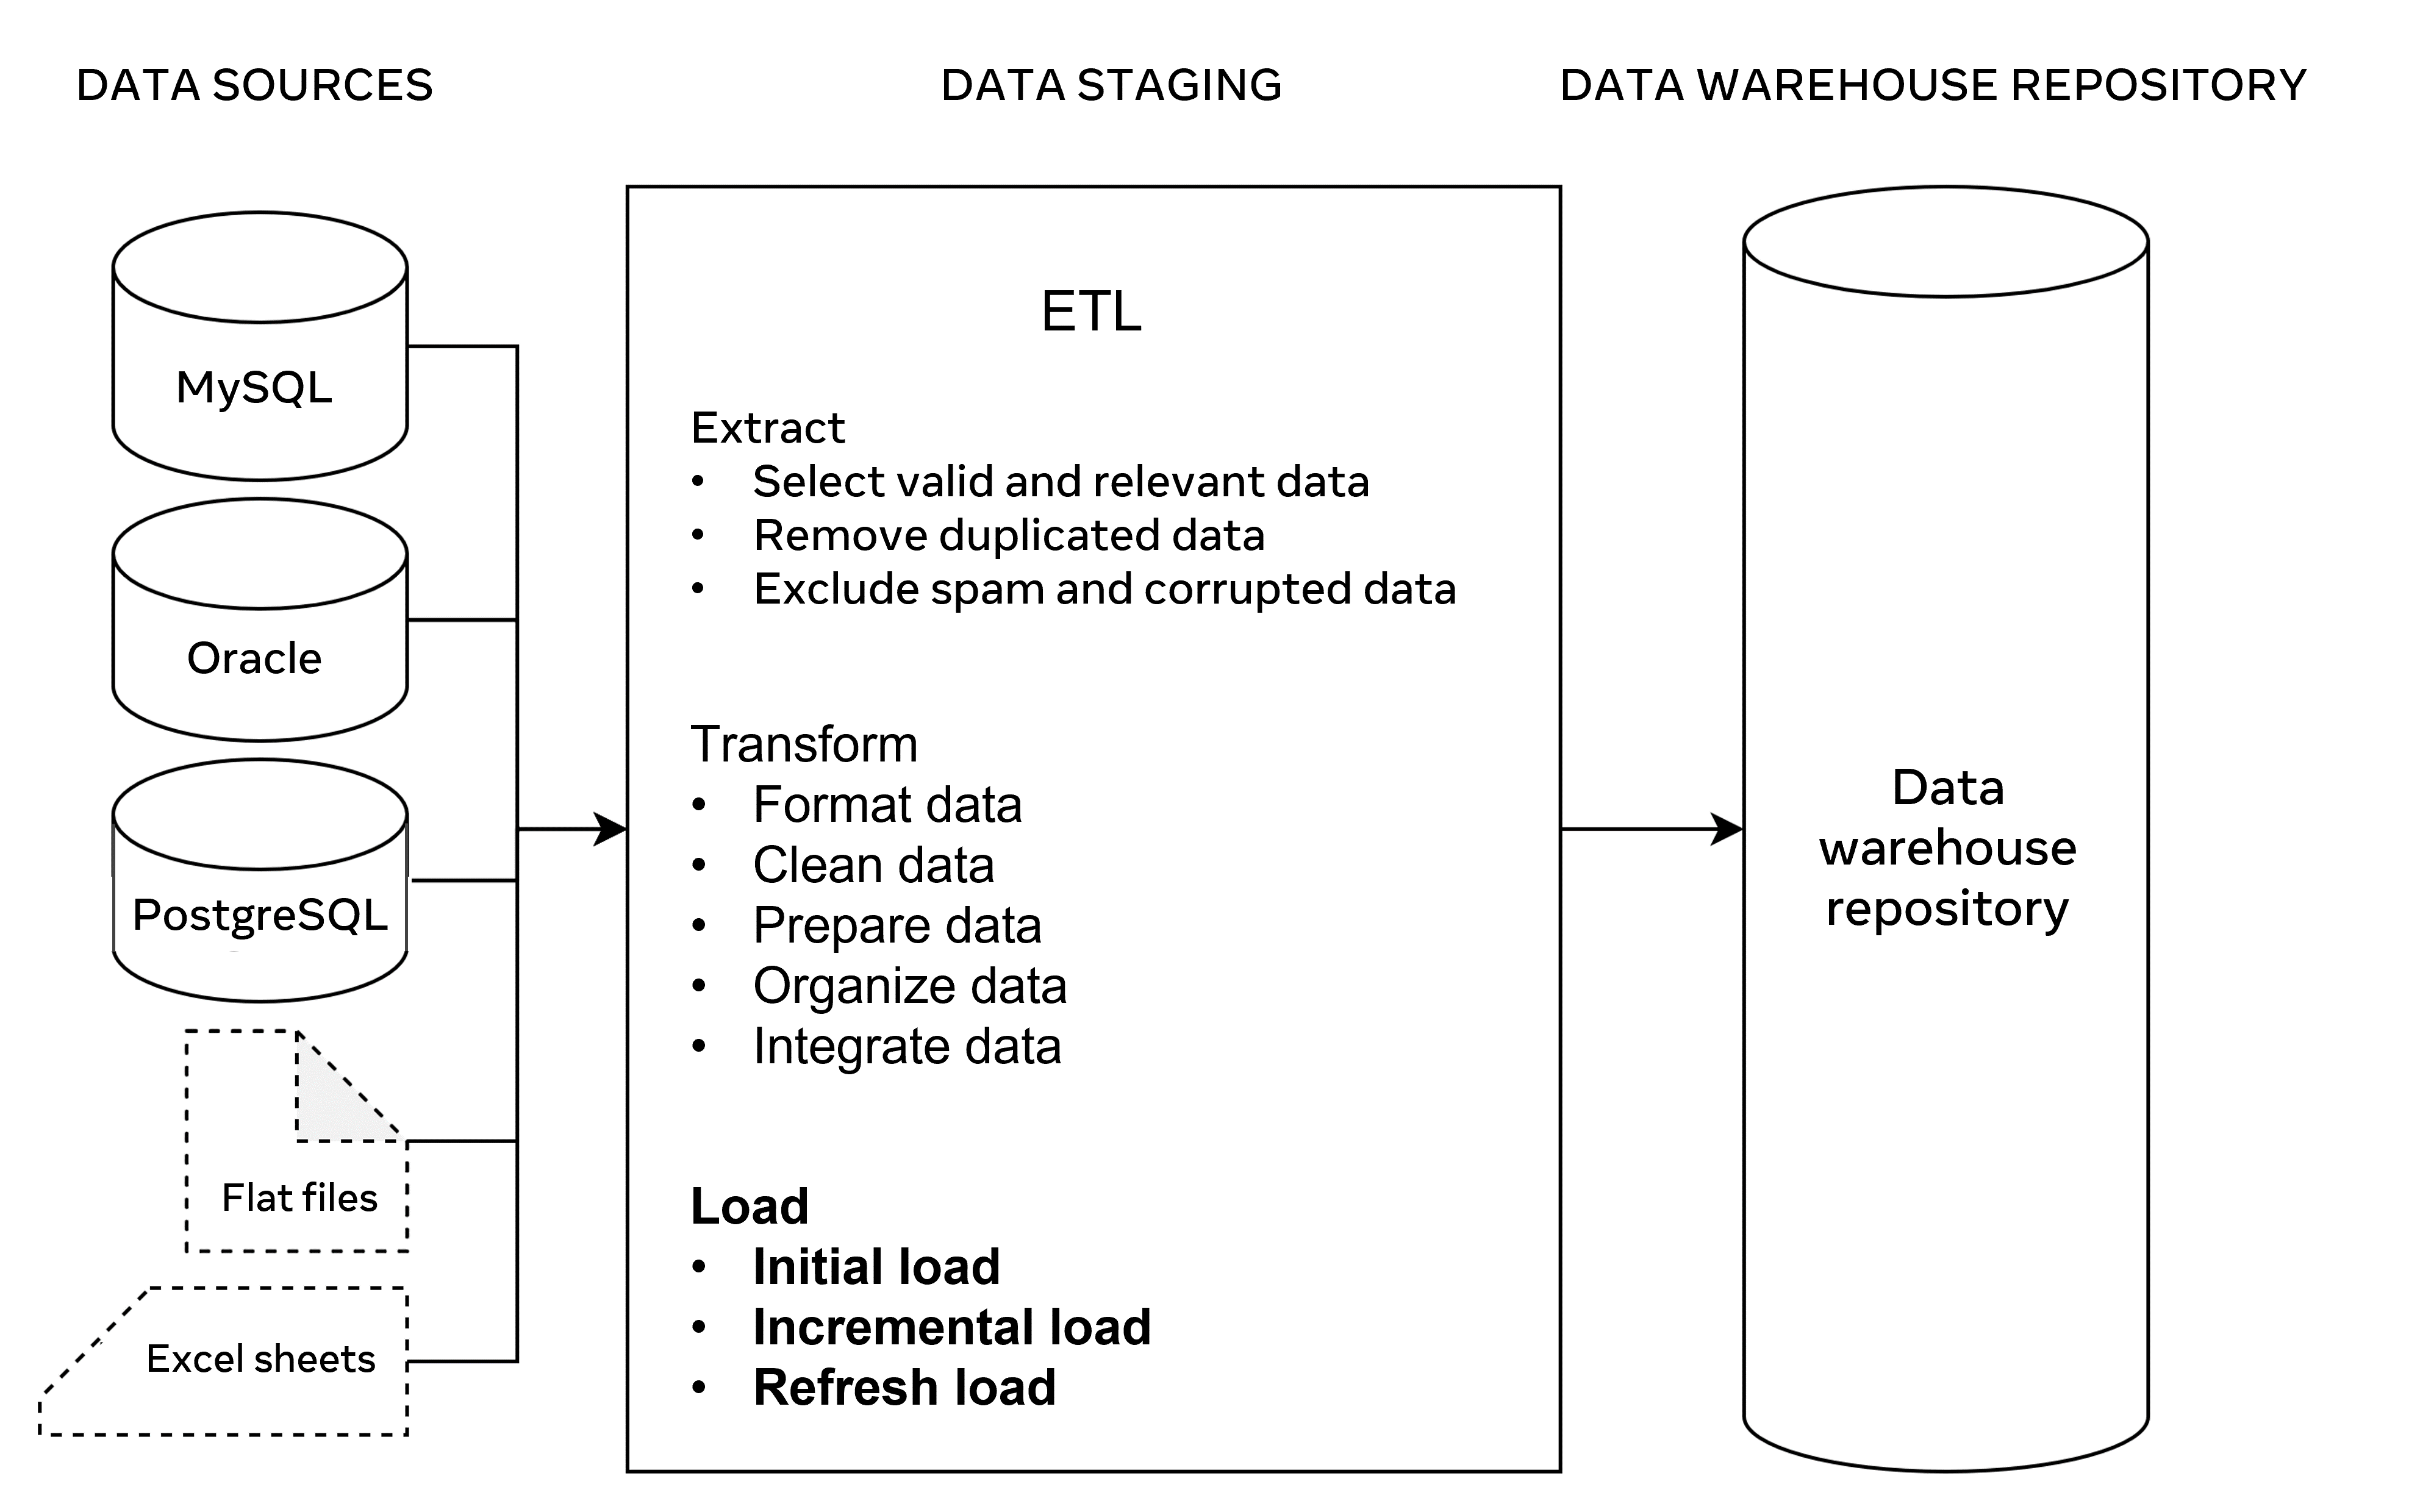
\includegraphics[width=0.8\textwidth]{./Picts/etls3.png}
    \caption{}
\end{figure}

\subsubsection{ETL Tools}
Ada beberapa alat yang tersedia yang dapat Anda gunakan untuk melaksanakan proses ETL ini. Alat-alat ini mengotomatisasi proses ekstraksi, transformasi, dan pemuatan data ke tingkat yang lebih canggih. Beberapa contoh alat-alat tersebut antara lain:
\begin{itemize}
    \item Oracle: Database terkemuka di industri yang menawarkan berbagai pilihan solusi data warehouse.
    \item Amazon RedShift: Alat data warehouse yang sederhana dan hemat biaya yang dapat digunakan untuk menganalisis berbagai jenis data.
    \item MarkLogic: Solusi data warehouse yang memudahkan dan mempercepat integrasi data dibandingkan alat lain. Ia dapat mengakses berbagai jenis data seperti data mesin pencari, file teks, dan RDF.
\end{itemize}

\subsection{Tujuan dan Tantangan ETL}
Tujuan:
\begin{itemize}
    \item ETL bertujuan untuk menggabungkan berbagai sumber data atau mengabstraksi sumber data besar agar lebih mudah diakses oleh konsumen data.
    \item Proses ini memungkinkan penyimpanan data mentah sebagai cadangan di warehouse, sambil menyediakan data yang telah diproses untuk penggunaan saat dibutuhkan.
\end{itemize}
Tantangan:
\begin{itemize}
    \item Mengelola volume data yang besar dan beragam bisa menjadi tantangan. Memastikan pipeline selalu diperbarui dan data tersedia saat dibutuhkan adalah kunci.
    \item Perubahan pada database dapat memicu kebutuhan untuk memperbarui pipeline ETL, yang memerlukan pemahaman yang kuat tentang kebutuhan dan tujuan pipeline tersebut.
\end{itemize}

Pemangku kepentingan harus memiliki pemahaman yang baik tentang pipeline ETL dan bertanggung jawab untuk melakukan perubahan yang diperlukan saat ada pembaruan.

ETL pipelines adalah komponen fundamental dalam dunia big data, cloud computing, dan metaverse, membantu dalam pengelolaan dan akses data yang efisien.

\subsection{ETL Testing}
\subsubsection{Overview}
Data warehouse menyediakan repositori data terpusat yang mendukung analisis data canggih dan pelaporan. ETL merujuk pada proses Ekstrak, Transformasi, dan Pemuatan yang diperlukan untuk memindahkan data dari berbagai sumber data ke dalam data warehouse.

Untuk menyelesaikan proses ETL, Anda perlu:
\begin{itemize}
    \item Mengekstrak data yang relevan dan valid.
    \item Mengubah data yang diekstrak menjadi format dan struktur yang sesuai.
    \item Dan memuat data yang telah diubah dari berbagai sumber data ke dalam repositori data warehouse.
\end{itemize}

Namun, bagaimana Anda dapat memastikan bahwa data yang dimuat benar, valid, andal, dan konsisten?

\subsubsection{ETL Testing}
Tujuan utama pengujian ETL adalah untuk memastikan akurasi, keandalan, validitas, dan konsistensi data yang dimuat. Pengujian ETL memeriksa apakah ada masalah dalam proses ETL yang menghalangi pembentukan data berkualitas baik. Hal ini dapat dilakukan dengan melaksanakan tindakan berikut:
\begin{itemize}
    \item Pemetaan data secara tepat.
    \item Memvalidasi data.
    \item Memeriksa duplikat data.
    \item Memvalidasi tanggal.
    \item Dan memverifikasi kelengkapan dan keakuratan data.
\end{itemize}

\subsubsection{ETL Testing in Practice}
Global Super Store memiliki banyak departemen yang berbeda, masing-masing mengelola data pelanggan dengan cara yang berbeda di server yang berbeda menggunakan identifikasi unik yang berbeda. Misalnya, departemen penjualan menggunakan nomor telepon pelanggan sebagai identifikasi unik, sementara departemen pemasaran menggunakan identifikasi pelanggan yang dihasilkan secara otomatis.

Selain itu, beberapa data diwakili dengan cara yang berbeda. Misalnya, nama lengkap pelanggan dinyatakan sebagai satu kolom di departemen penjualan. Namun, di departemen pemasaran, nama lengkap pelanggan dinyatakan dalam dua kolom (sebagai nama depan dan nama belakang). Tanggal di departemen penjualan diformat sebagai \verb|yyyy-m-d| (misalnya \verb|2020-9-5|). Namun, di departemen pemasaran, tanggal diformat sebagai \verb|yy\m\d| (atau \verb|20\9\5|).

Hal ini menimbulkan beberapa masalah bagi Global Super Store. Masalah utama yang tidak dapat mereka selidiki adalah siapa pelanggan yang melakukan pemesanan setelah kampanye pemasaran terbaru mereka, karena ID pelanggan disimpan dalam format yang berbeda di berbagai departemen. Solusi untuk masalah ini adalah membuat model database baru di data warehouse. Mereka kemudian dapat mengekstrak data yang relevan, mentransformasikannya, dan memuatnya dari database penjualan dan pemasaran.

Model baru ini dapat mencakup:
\begin{itemize}
    \item Tabel Pesanan dengan ID pesanan dan tanggal pesanan.
    \item Tabel Pemasaran dengan ID pemasaran dan tanggal pemasaran.
    \item Dan tabel pelanggan dengan nama lengkap setiap pelanggan, identifikasi unik awal dari kedua departemen, dan kunci unik baru yang memungkinkan identifikasi pelanggan dari kedua departemen.
\end{itemize}

Model baru ini memungkinkan untuk menghubungkan riwayat pembelian pelanggan dengan kampanye pemasaran, dan kemudian melakukan analisis data yang relevan.

\subsubsection{Performing ETL Testing}
Untuk memastikan bahwa data telah dimuat dengan benar, pengujian ETL harus dilakukan menggunakan metode-metode berikut.
\begin{itemize}
    \item Dokumen pemetaan data

          Buat dokumen pemetaan data untuk mentransformasi data dari sumber data kedua departemen ke repositori tujuan di data warehouse. Dokumen ini harus direview, diverifikasi, dan divalidasi oleh insinyur database dan analis data untuk memastikan pemetaan data yang benar.

    \item Validasi data

          Lakukan validasi data dengan membandingkan struktur data, tipe data, format data, dan batasan dalam tabel sumber dan tujuan yang terkait dengan dokumen pemetaan yang sesuai. Anda juga harus melakukan validasi data untuk memverifikasi nilai tanggal saat membuat catatan data baru, karena hal ini memungkinkan sistem data warehouse untuk mengekstrak data baru dari sumber data dan memperbarui basis data repositori yang relevan jika terjadi perubahan data.

    \item Kelengkapan data

          Pastikan kelengkapan data dengan memverifikasi bahwa semua data yang diharapkan telah dimuat ke dalam tabel tujuan, termasuk jumlah catatan dan catatan yang ditolak. Anda juga perlu memeriksa batasan yang telah diterapkan dan memastikan bahwa semua nilai unik telah diisi sesuai persyaratan.

    \item Kebenaran data

          Lakukan verifikasi kebenaran data untuk menyelesaikan konflik penamaan data, pastikan semua data yang salah eja telah diperbaiki, dan pastikan nilai data yang tidak terduga (artinya, nilai yang di luar rentang) telah diperbaiki atau dihapus.

    \item Kualitas data

          Pastikan kualitas data yang baik dengan memeriksa nama dan format angka, presisi, serta nilai null di mana batasan NOT NULL telah ditentukan.

    \item Data unik

          Lakukan pemeriksaan duplikat untuk memastikan semua tabel memiliki catatan data yang unik dan semua catatan data duplikat telah dihapus.
\end{itemize}

\subsection{Konsep Dasar Dimensional Data Modeling}
\begin{itemize}
    \item \textbf{Dimensi}: Elemen yang berbeda dari data yang memberikan konteks untuk ukuran. Contoh: waktu dan lokasi dalam database Global Superstore.
    \item \textbf{Fakta}: Data yang dapat diukur dan dihitung dalam database. Contoh: jumlah produk yang terjual dan keuntungan yang diperoleh.
\end{itemize}

\subsection{Struktur Dimensional Data Model}
\begin{itemize}
    \item Tabel Dimensi: Menyimpan elemen data dimensi dan dapat disusun dalam hierarki untuk analisis data yang lebih mendalam.
    \item Tabel Fakta: Menyimpan ukuran data. Contoh: tabel fakta penjualan yang terhubung dengan tabel dimensi seperti pemasok, pelanggan, produk, waktu, dan lokasi.
\end{itemize}

\subsection{Jenis Ukuran dalam Tabel Fakta}
\begin{itemize}
    \item Stored Measures: Ukuran yang disimpan dalam data warehouse, seperti data penjualan dan harga produk.
    \item Calculated Measures: Ukuran yang dihitung dari ukuran lain, misalnya, keuntungan dihitung dengan mengurangi biaya produk dari harga jual.
\end{itemize}

\subsection{Skema dalam Dimensional Data Modeling}
\begin{itemize}
    \item Star Schema:

          \begin{figure}[H]
              \centering
              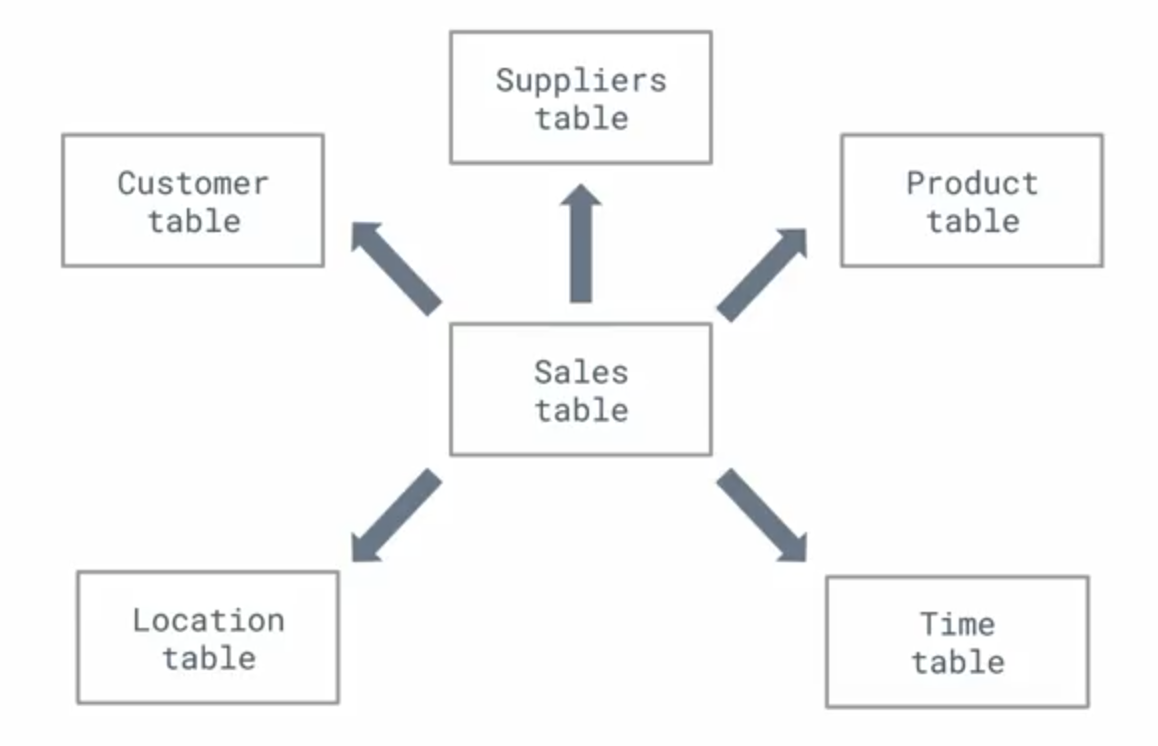
\includegraphics[width=0.8\textwidth]{./Picts/starschema.png}
              \caption{}
          \end{figure}
          Model sederhana yang terdiri dari tabel fakta di tengah yang terhubung dengan satu atau lebih tabel dimensi. Contoh: tabel fakta penjualan terhubung dengan tabel dimensi pemasok, pelanggan, produk, waktu, dan lokasi.

          \begin{figure}[H]
              \centering
              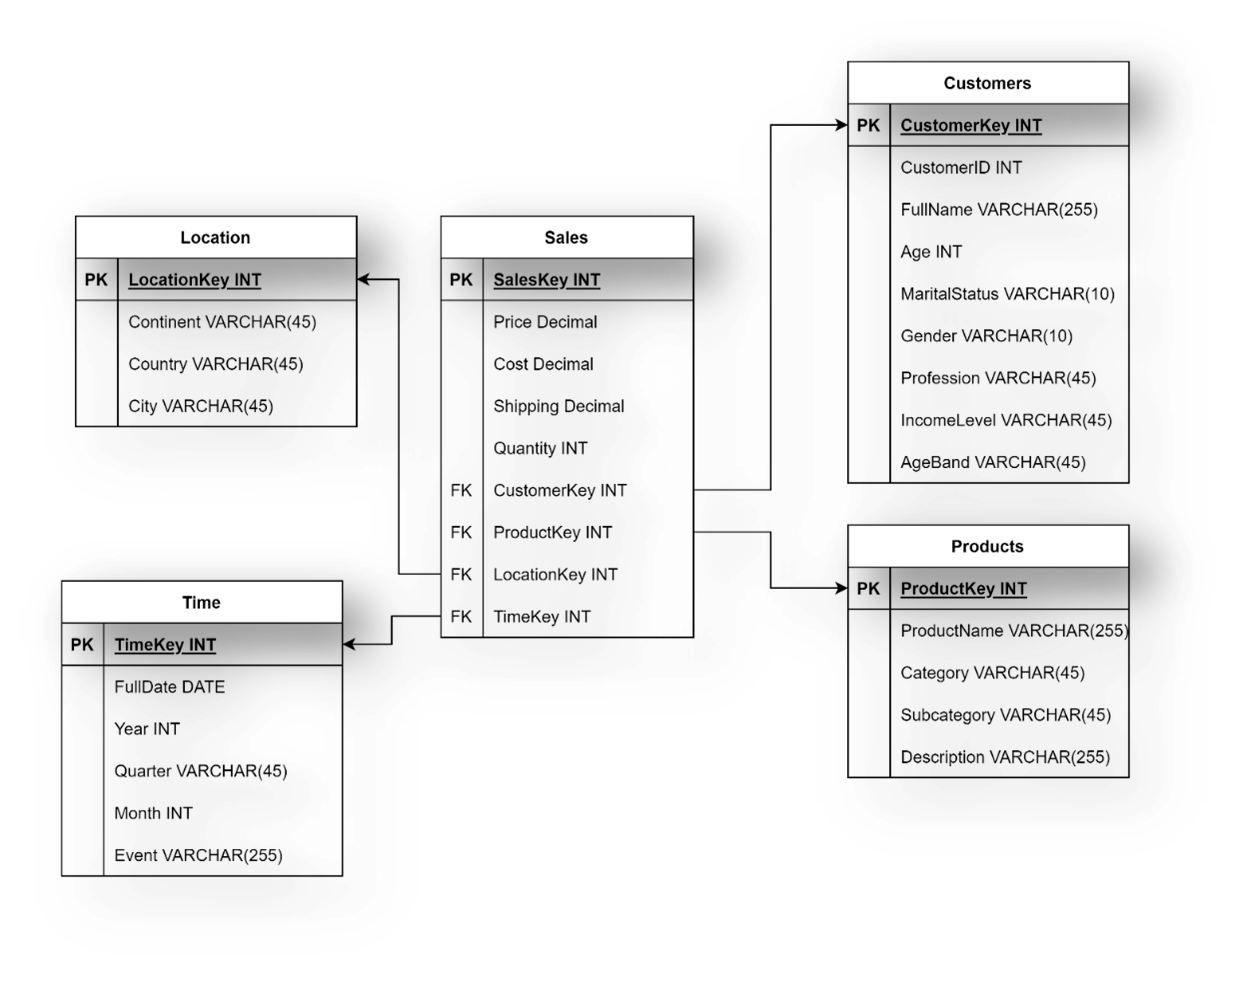
\includegraphics[width=0.8\textwidth]{./Picts/starexample.png}
              \caption{}
          \end{figure}
    \item Snowflake Schema:

          \begin{figure}[H]
              \centering
              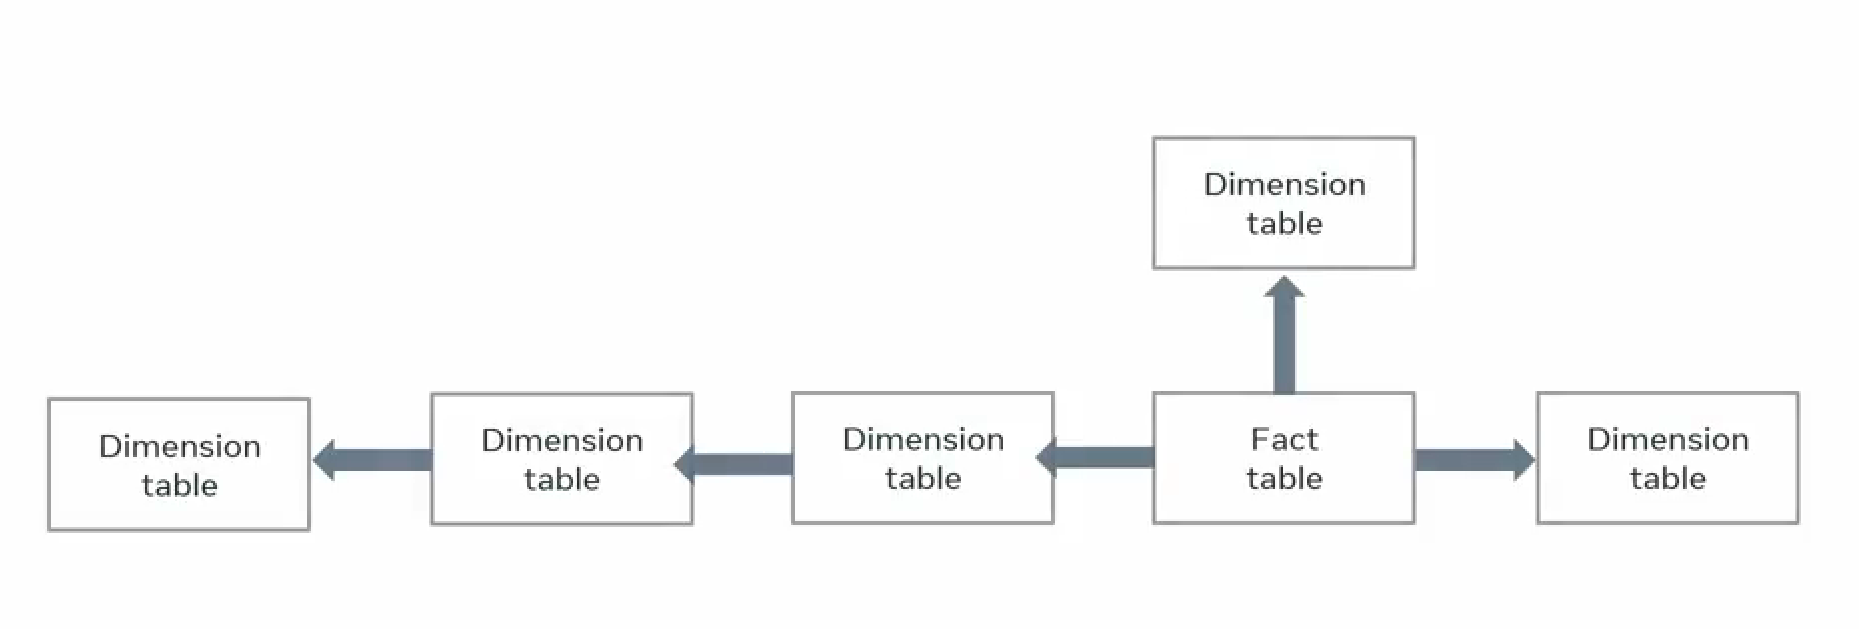
\includegraphics[width=0.8\textwidth]{./Picts/snowflakeschema.png}
              \caption{}
          \end{figure}
          Skema yang lebih kompleks di mana tabel dimensi dinormalisasi untuk menghilangkan redundansi data. Contoh: tabel produk dinormalisasi menjadi tabel produk, subkategori, dan kategori.

          \begin{figure}[H]
              \centering
              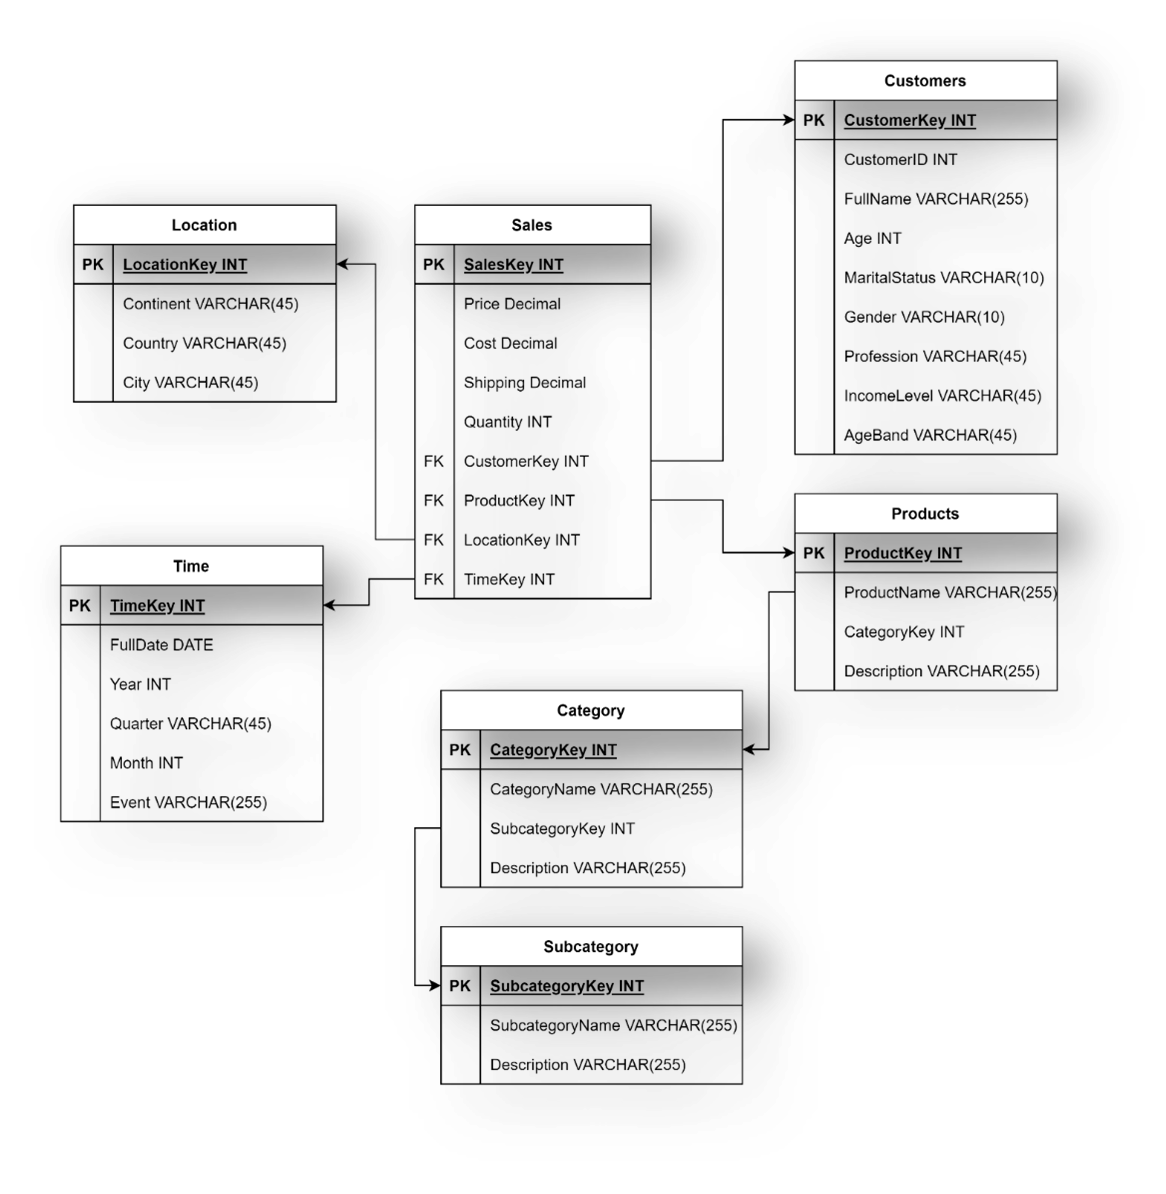
\includegraphics[width=0.8\textwidth]{./Picts/snowflakeexample.png}
              \caption{}
          \end{figure}
\end{itemize}

\subsection{Praktik Terbaik dalam Mendesain Data Model Warehouse}
Tentukan aktivitas bisnis yang ingin dianalisis dan dimensi yang memberikan konteks yang paling berarti.

Organisasi data harus mudah dipahami, diakses, dan di-query.

\subsection{Kubus OLAP}
\subsubsection{Overview}
OLAP Data warehouses mengumpulkan dan mengintegrasikan data dari berbagai sumber data. Data ini diimpor dari sistem basis data Pemrosesan Transaksi Online (OLTP), di mana data disusun untuk mengelola operasi bisnis sehari-hari secara real-time.

Misalnya, Global Super Store menjual produk secara online ke seluruh dunia. Oleh karena itu, perusahaan ini memerlukan sistem basis data OLTP untuk mengumpulkan, memperbarui, mengambil, dan mencadangkan data pelanggan, produk, dan pesanan. Jenis basis data ini tidak terlalu efektif dalam melakukan analisis data. cubes

Untuk melakukan analisis data yang efektif pada basis data OLTP, Anda perlu merestrukturisasi data Anda ke dalam sistem basis data OLAP (Online Analytical Processing) yang dirancang khusus untuk analisis data. Keuntungan utama dari sistem basis data OLAP meliputi hal-hal berikut:
\begin{itemize}
    \item Mereka memudahkan analisis multidimensi.
    \item Mereka menyediakan alat untuk akses dan penyaringan data multidimensi dengan mudah.
    \item Dan mereka mendukung pengambilan data dalam jumlah besar dengan cepat.
\end{itemize}

Fitur-fitur ini memungkinkan analis data untuk menyediakan tingkat analisis data yang dioptimalkan, yang membantu audiens mereka mendapatkan jawaban atas pertanyaan mereka mengenai kinerja bisnis. Dalam hal ini, sistem basis data OLAP menggunakan struktur kubus untuk memvisualisasikan konsep data multidimensi. Kubus OLAP adalah array multidimensi yang digunakan untuk menyimpan dan memelihara data guna menyediakan tingkat analisis data yang lebih canggih dengan wawasan yang lebih menarik.

\begin{figure}[H]
    \centering
    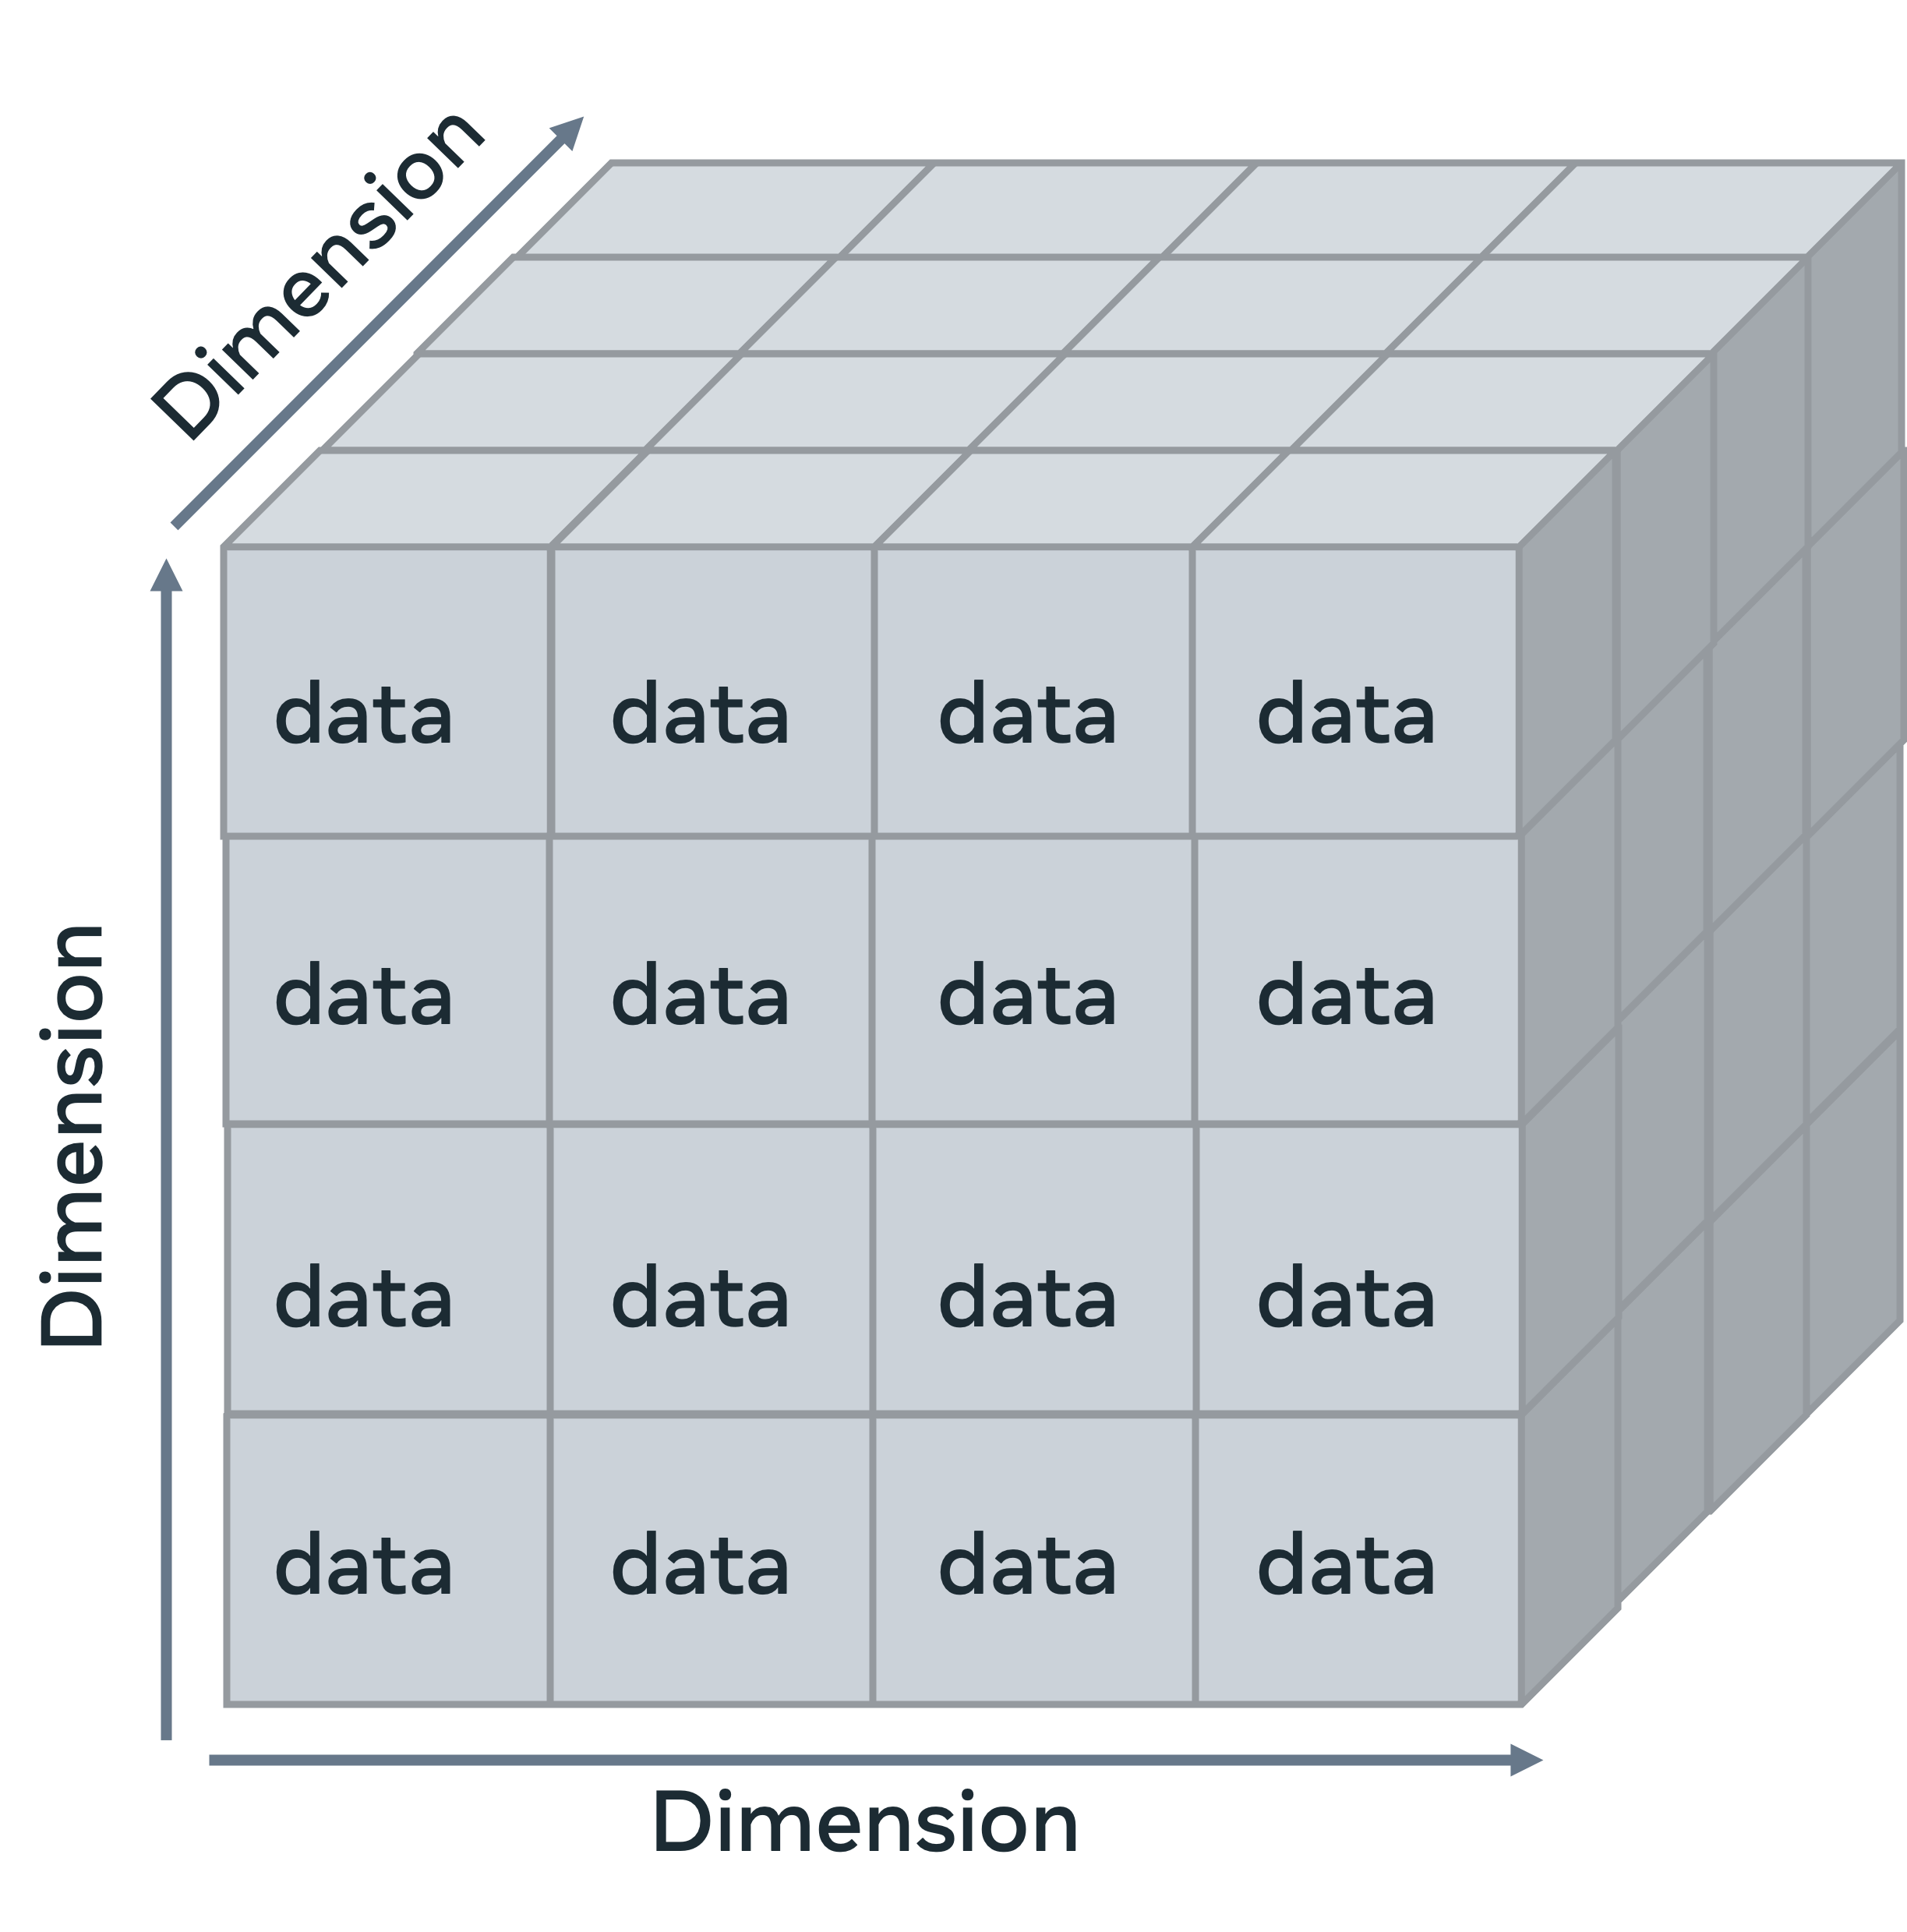
\includegraphics[width=0.8\textwidth]{./Picts/olapcube.png}
    \caption{}
\end{figure}

\subsubsection{Kubus Olap dalam Praktek}
Untuk melakukan analisis data, Anda perlu jelas tentang aktivitas bisnis mana yang ingin Anda teliti. Anda juga perlu mengetahui ukuran dan dimensi mana yang diperlukan untuk memberikan informasi yang paling bermakna dan berguna.

Misalnya, Global Super Store menjual furnitur, perlengkapan kantor, dan produk teknologi di seluruh dunia. Mereka ingin meneliti kinerja penjualan kategori produk yang berbeda selama empat tahun terakhir di empat negara Eropa yang berbeda: Prancis, Jerman, Italia, dan Inggris.

Salah satu solusi adalah menganalisis data perusahaan secara dasar, di mana Anda menyediakan Global Super Store dengan tiga tabel data sederhana yang menunjukkan total penjualan di setiap negara, total penjualan di setiap tahun, dan total penjualan di setiap kategori, seperti yang ditunjukkan di bawah ini.

\begin{figure}[H]
    \centering
    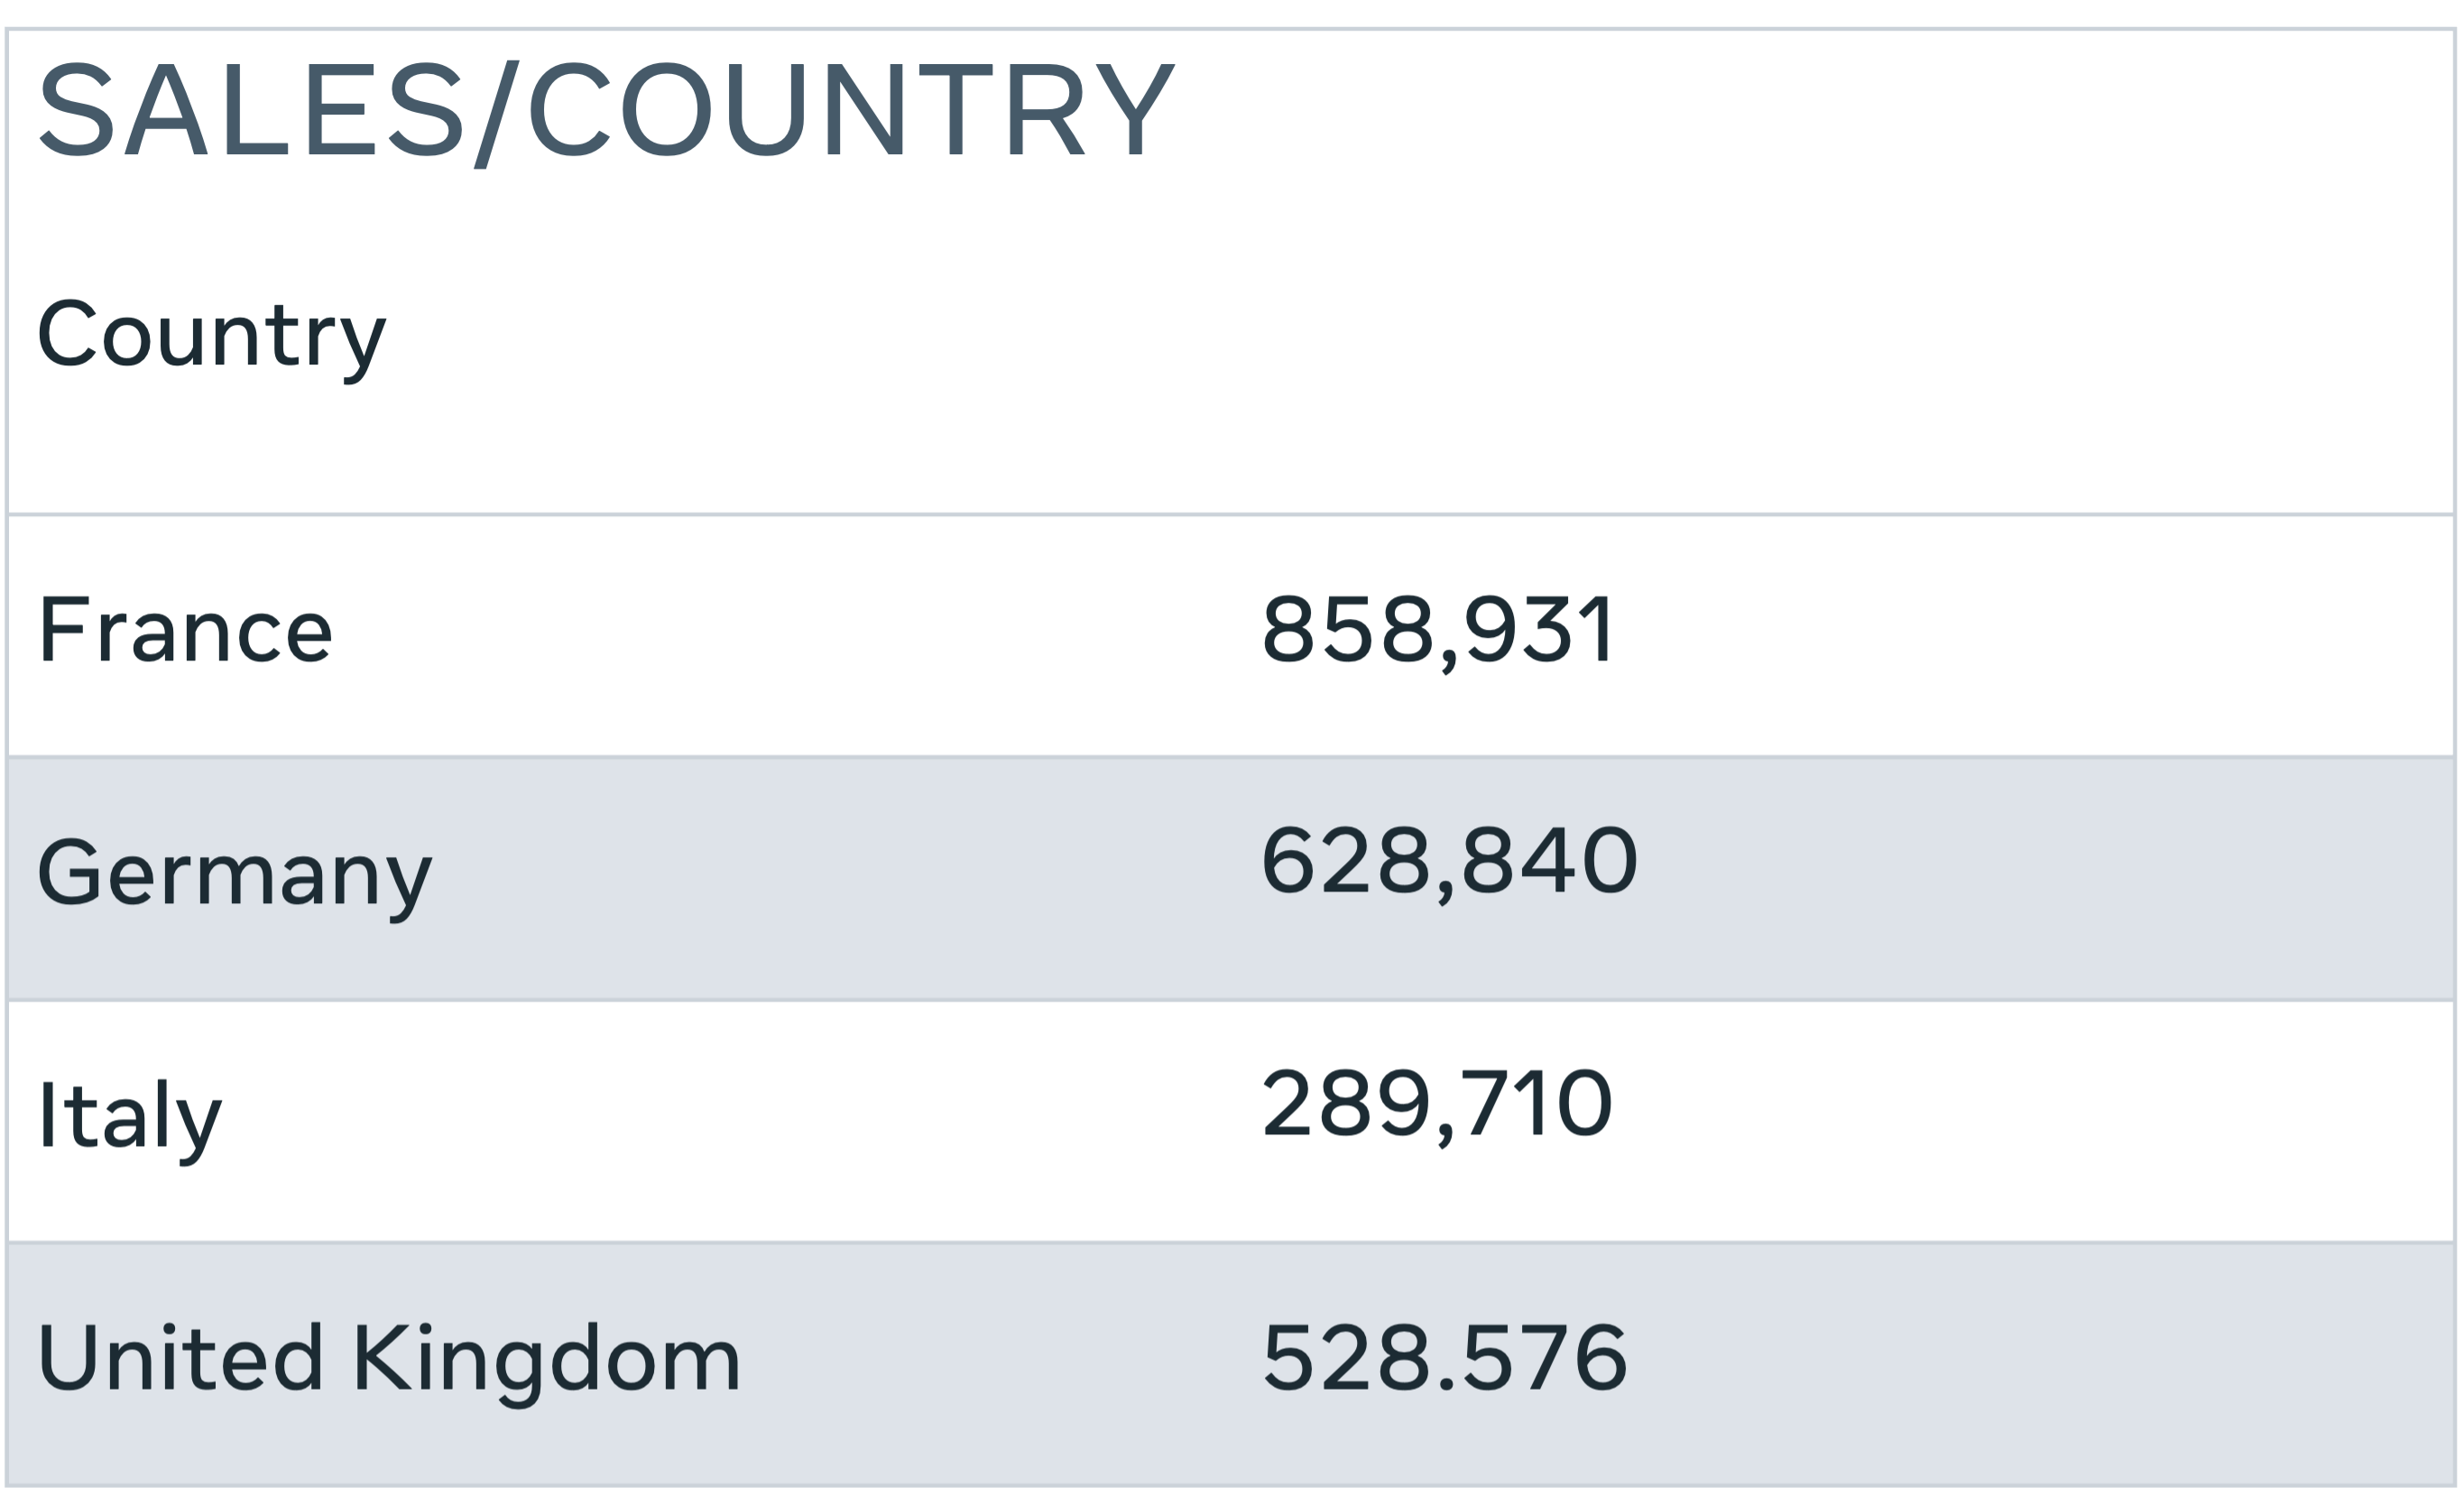
\includegraphics[width=0.8\textwidth]{./Picts/salescountry.png}
    \caption{}
\end{figure}

\begin{figure}[H]
    \centering
    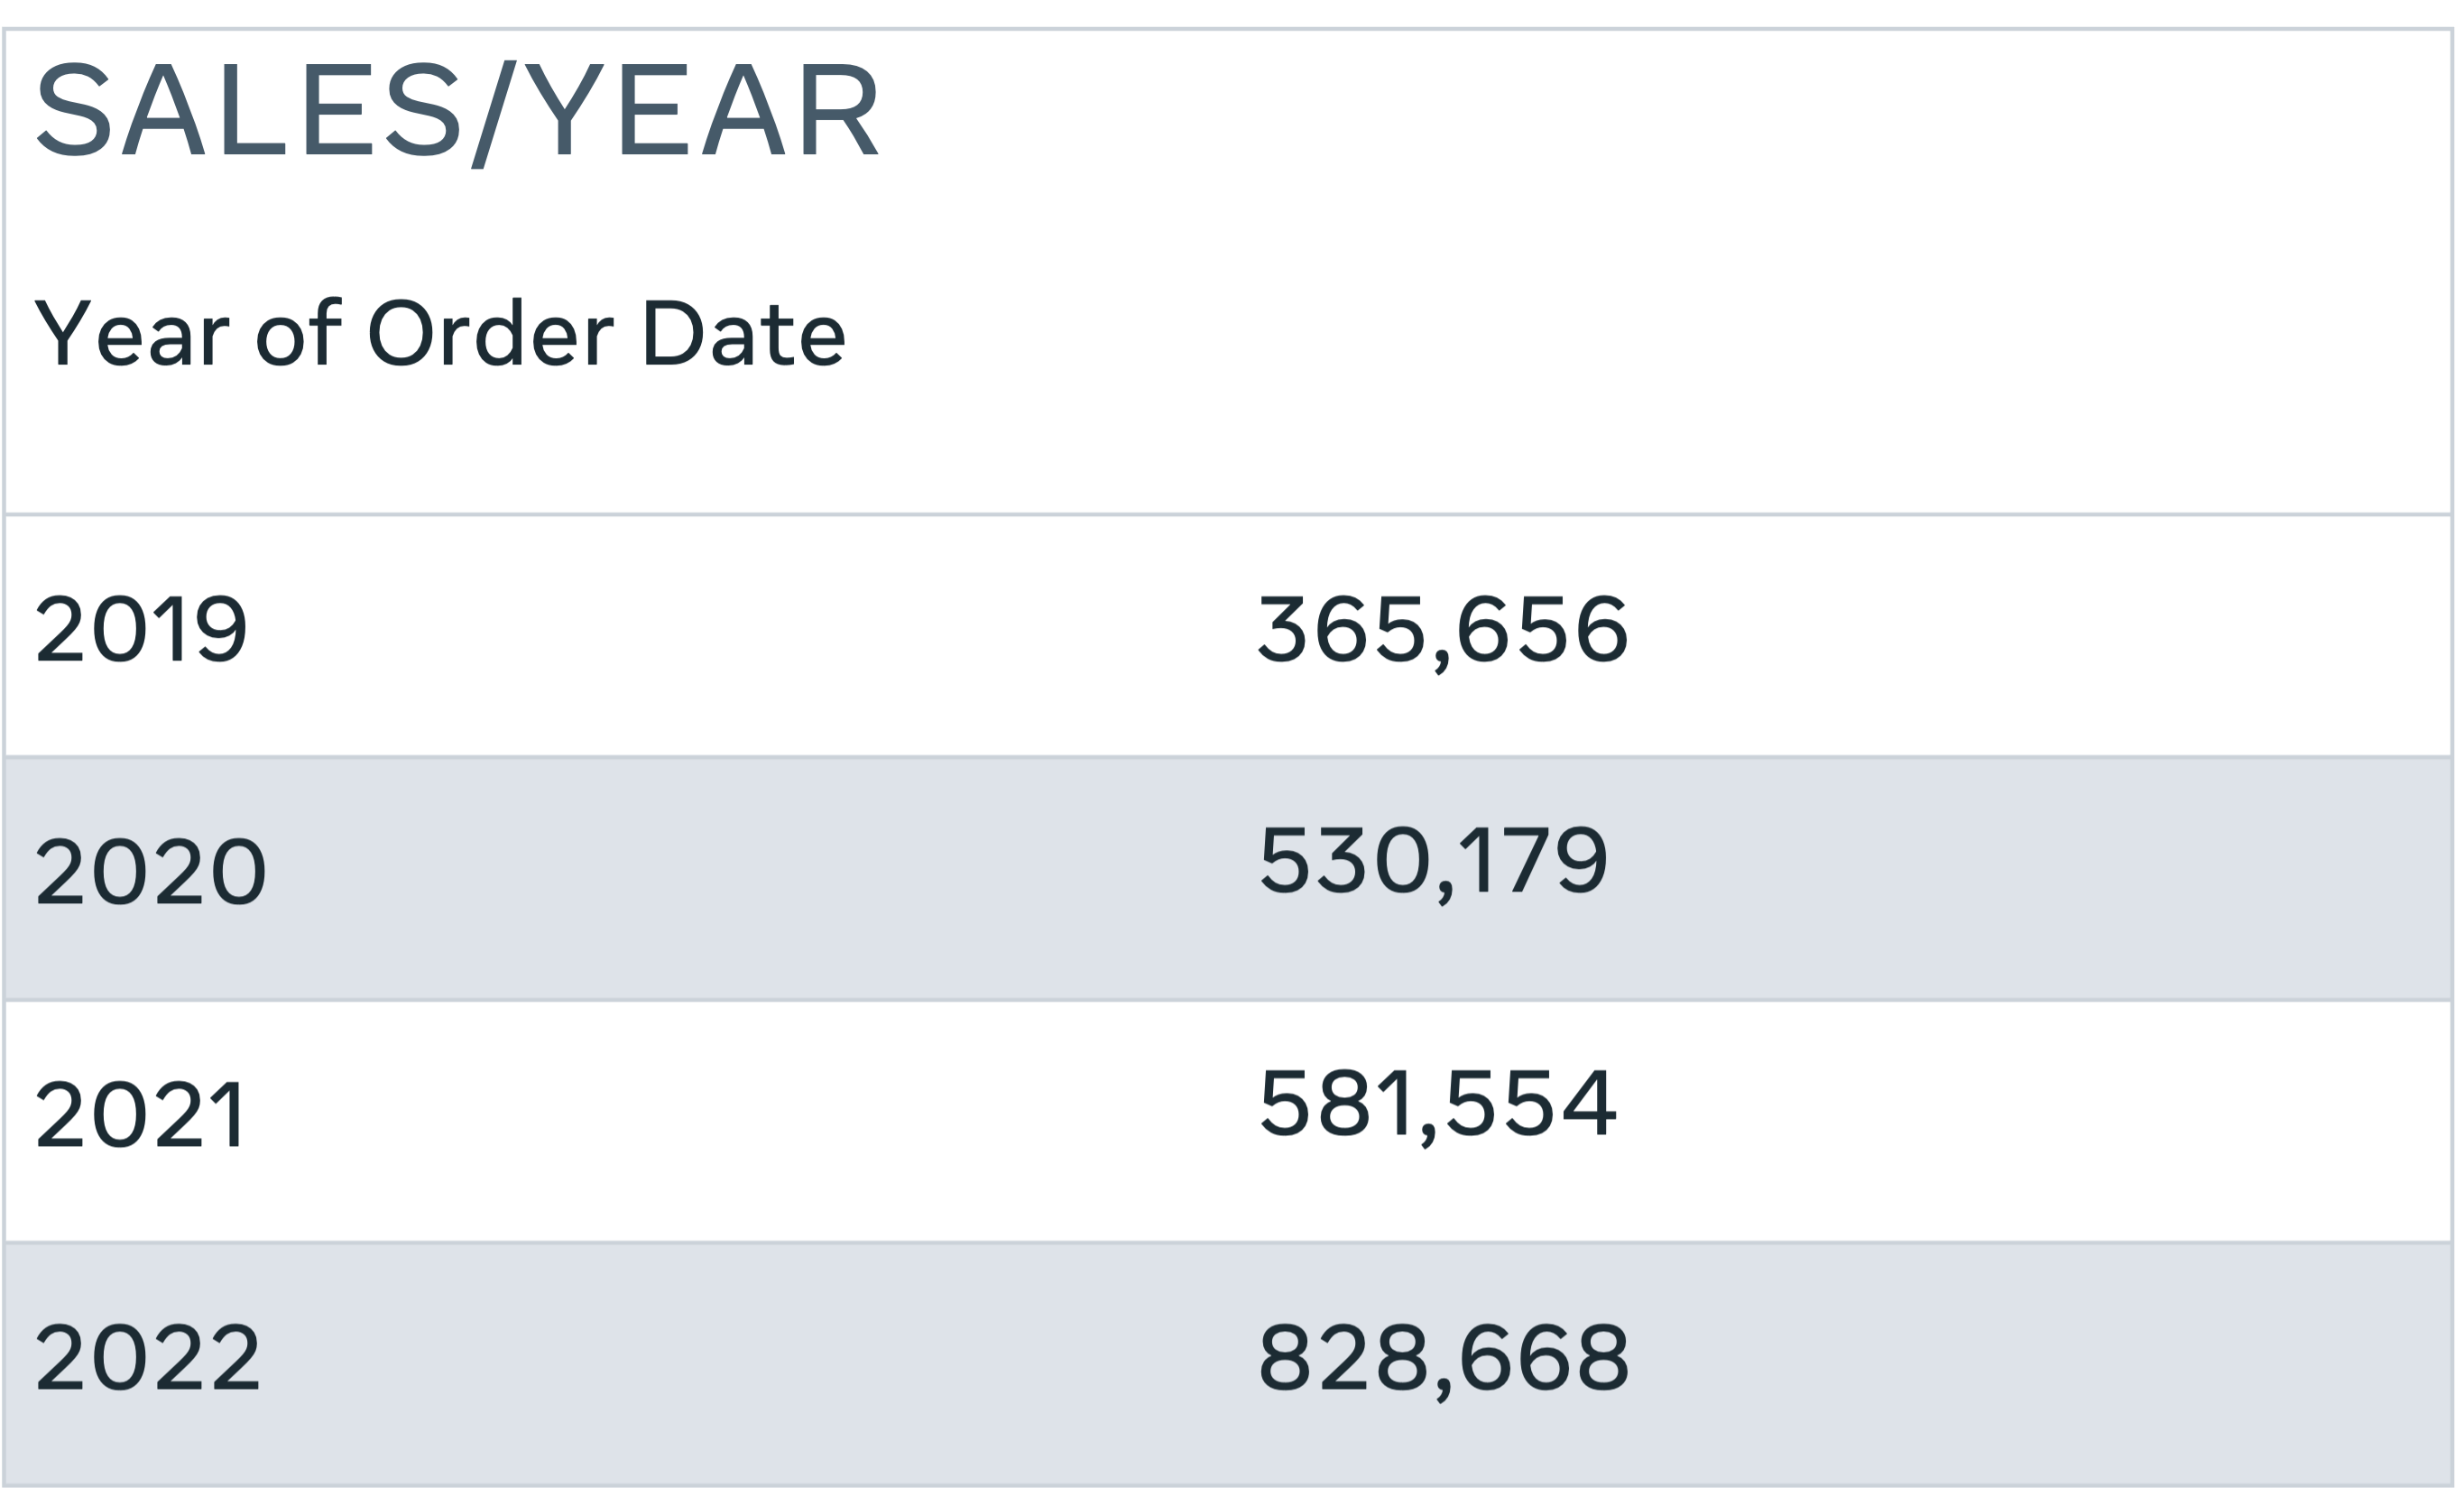
\includegraphics[width=0.8\textwidth]{./Picts/salesyear.png}
    \caption{}
\end{figure}

\begin{figure}[H]
    \centering
    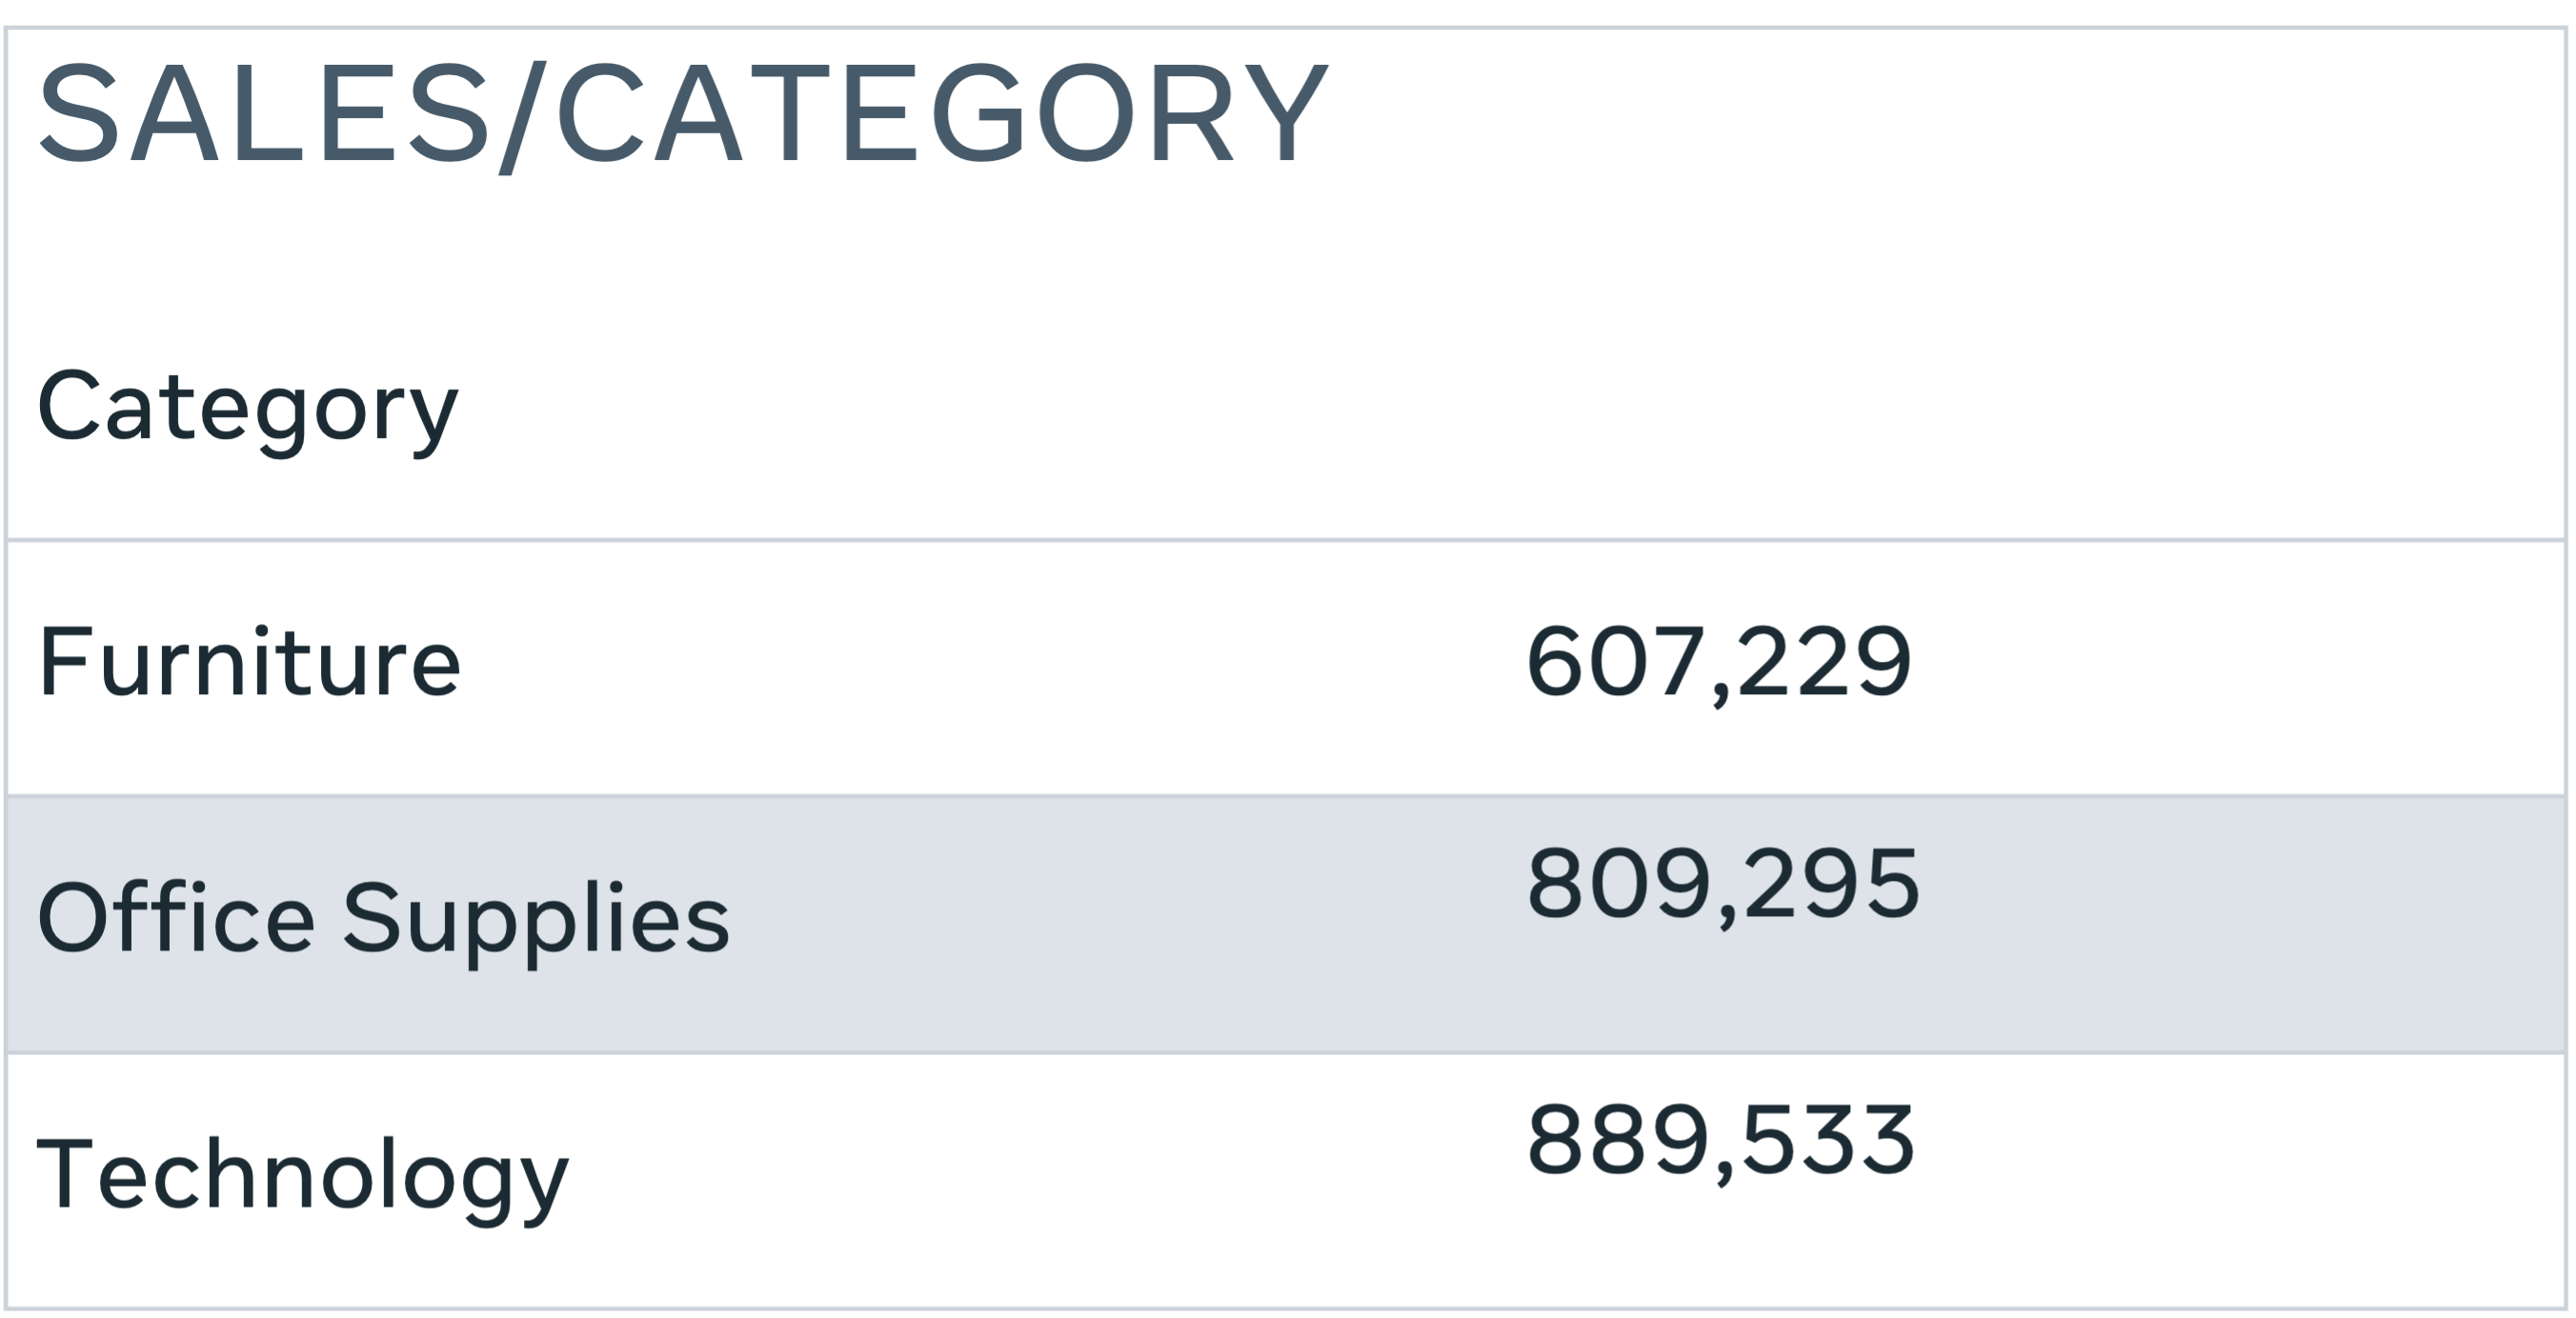
\includegraphics[width=0.8\textwidth]{./Picts/salescat.png}
    \caption{}
\end{figure}

Dalam setiap tabel data, Anda menampilkan total penjualan dalam konteks satu dimensi sebagai berikut:
\begin{itemize}
    \item Penjualan dalam konteks dimensi Waktu (Tahun – 2019, 2020, 2021, dan 2022).
    \item Penjualan dalam konteks dimensi Lokasi (Negara - Inggris, Italia, Prancis, dan Jerman).
    \item Penjualan dalam konteks dimensi Produk (Kategori - Furnitur, Perlengkapan Kantor, dan Teknologi).
\end{itemize}

Namun, jenis analisis ini tidak memberikan wawasan mendalam tentang data Anda. Dan tidak mudah untuk menganalisis dan membandingkan data berdasarkan dimensi yang berbeda-beda (yang diperlukan untuk memberikan informasi yang lebih menarik bagi pengambil keputusan bisnis). Di sinilah analisis data multidimensi dapat memainkan peran penting dengan menggunakan OLAP cube.

Dalam situasi ini, Anda dapat menggabungkan ketiga dimensi (Waktu, Lokasi, dan Produk) ke dalam sebuah kubus multidimensi seperti yang ditunjukkan di bawah ini.

\begin{figure}[H]
    \centering
    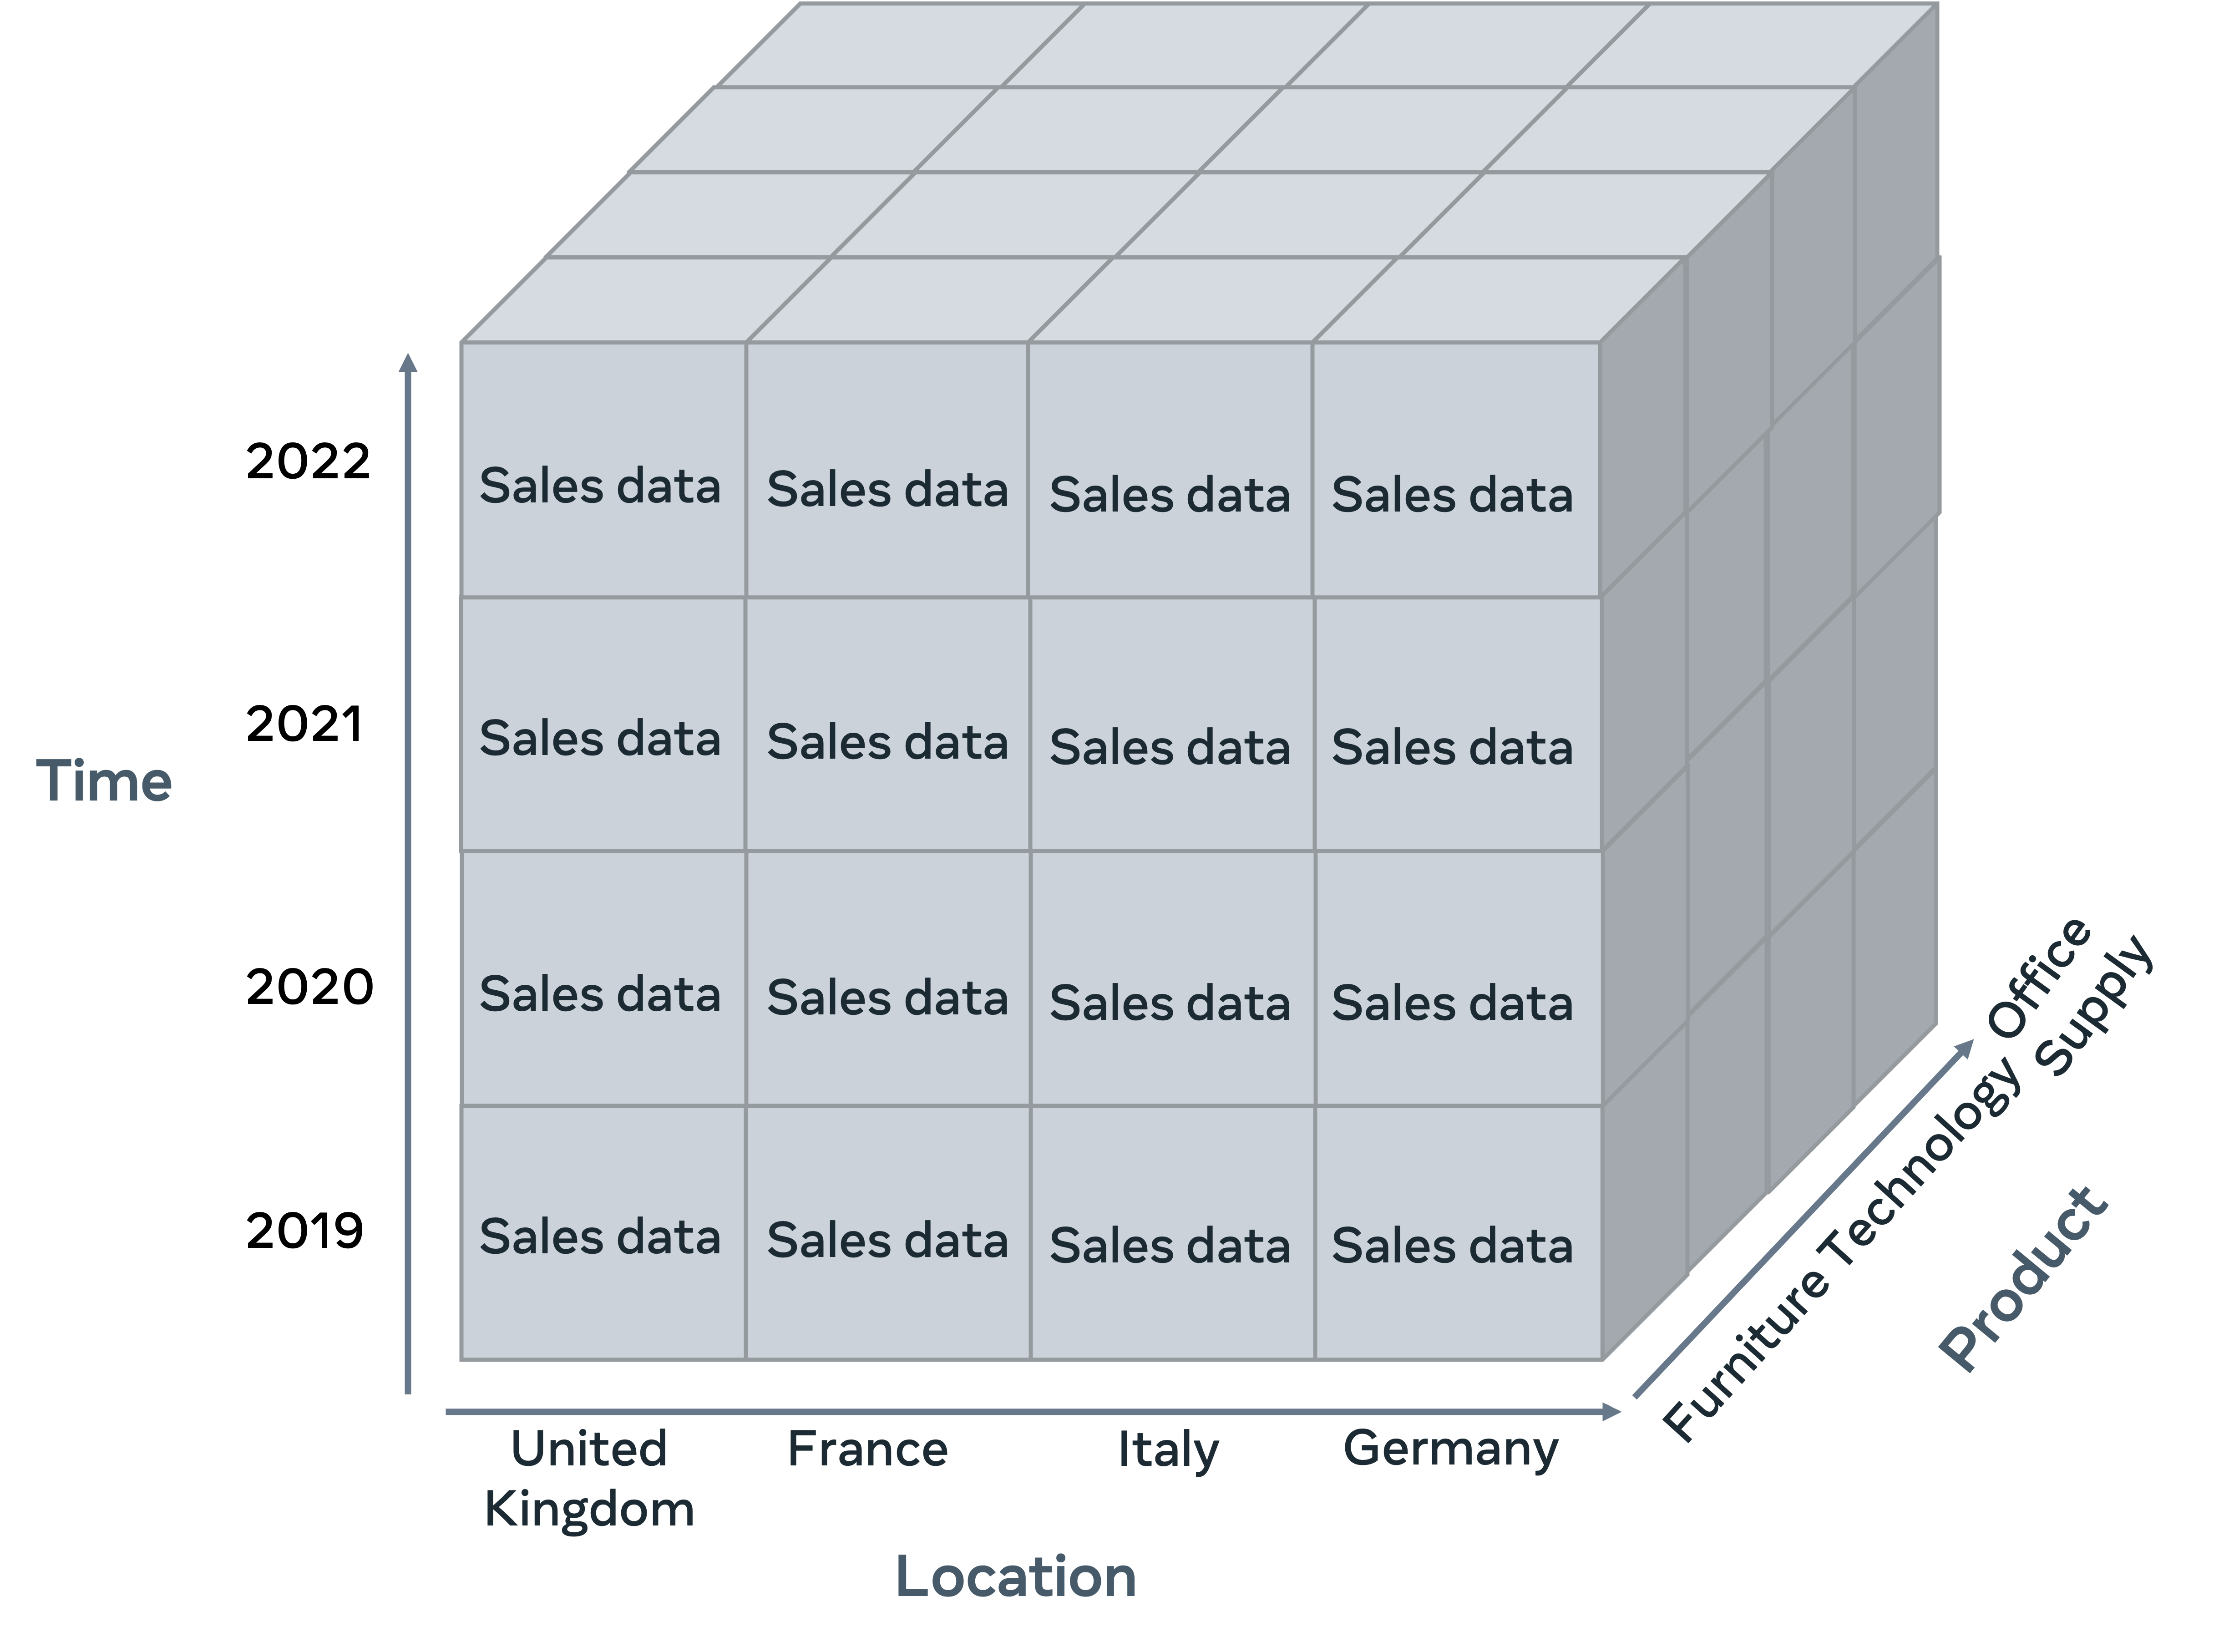
\includegraphics[width=0.8\textwidth]{./Picts/olapprac.png}
    \caption{}
\end{figure}

Anda kini dapat menggunakan OLAP cube untuk menganalisis data kompleks dengan lebih efisien. Anda dapat menemukan jawaban untuk pertanyaan apa pun yang Anda miliki tentang operasi penjualan bisnis berdasarkan dimensi yang berbeda (seperti produk, waktu, dan lokasi) secara bersamaan.

Sebagai contoh, grafik berikut menggabungkan ketiga dimensi tersebut untuk menunjukkan kinerja penjualan Global Super Store dalam hal semua kategori produk, selama empat tahun terakhir, di empat negara yang ditentukan:
\begin{figure}[H]
    \centering
    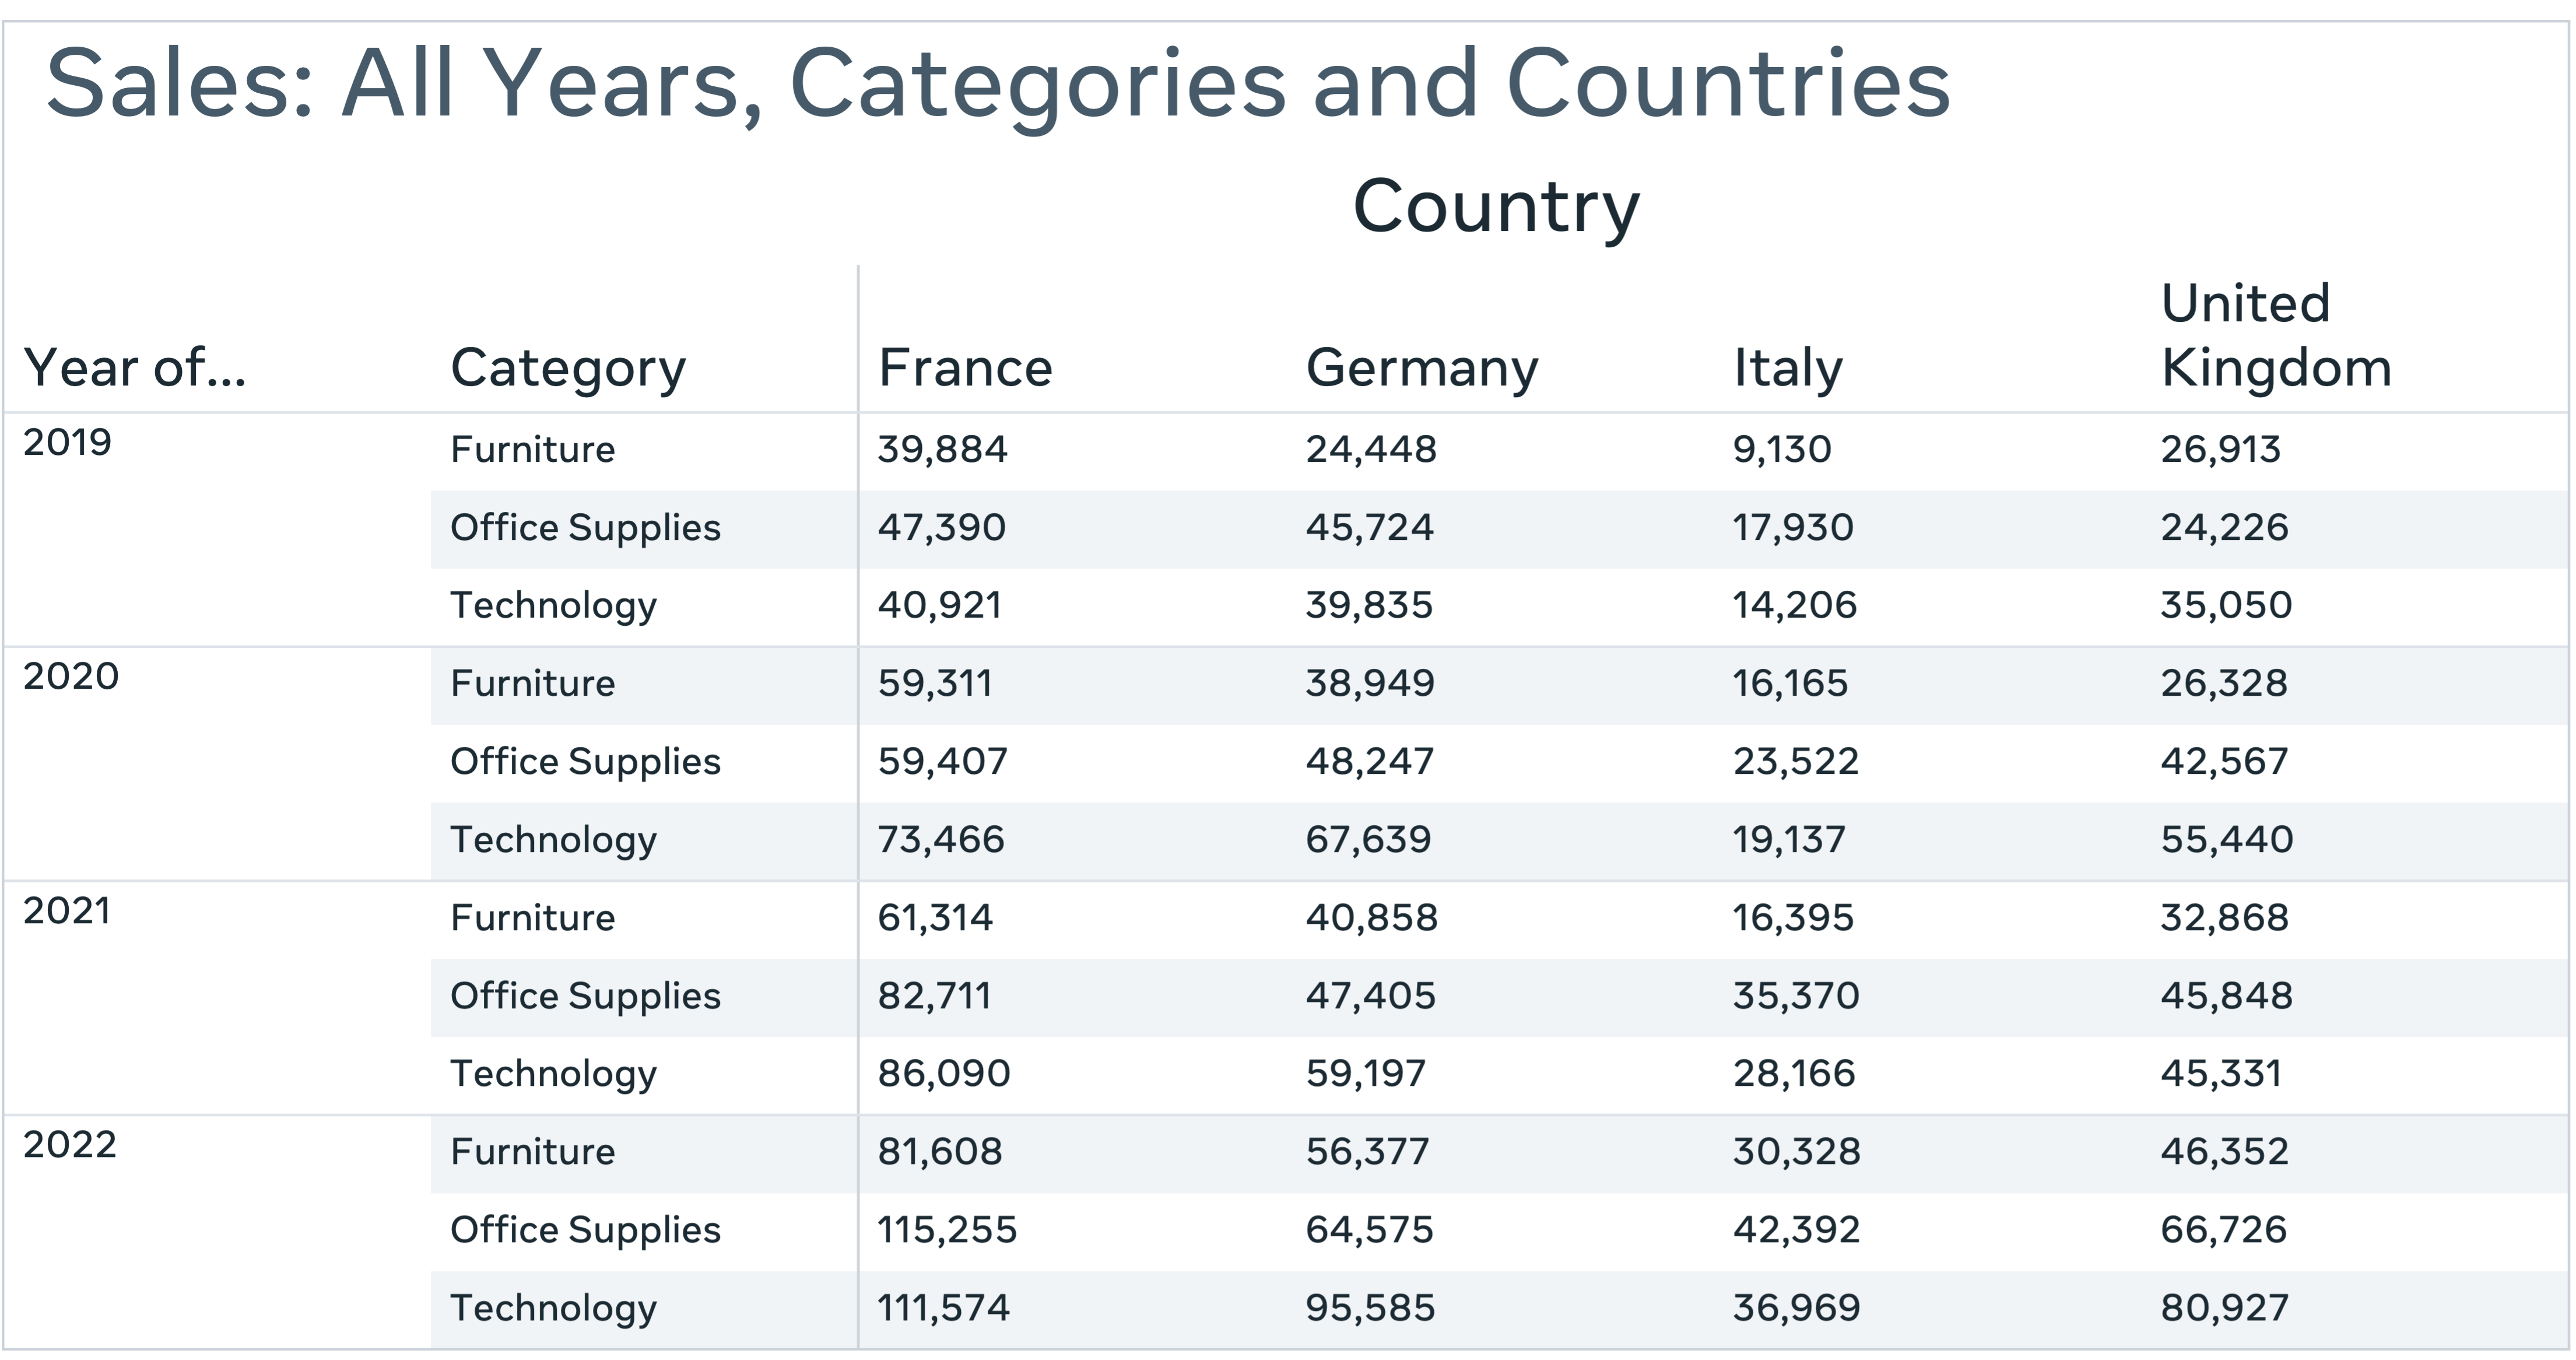
\includegraphics[width=0.8\textwidth]{./Picts/tabelolap.png}
    \caption{}
\end{figure}

Pada diagram multidimensi di atas, Anda sedang melihat data yang sama yang telah ditampilkan sebelumnya. Namun, kini Anda dapat dengan mudah membandingkan data tersebut. Misalnya, Anda dapat melihat bahwa penjualan tertinggi terjadi di Prancis untuk semua kategori produk, sementara Italia memiliki penjualan terendah. Anda mungkin juga telah memperhatikan bahwa terdapat peningkatan penjualan setiap tahun.

Seperti yang dapat Anda lihat, kubus multidimensi memudahkan metode yang lebih efisien untuk memberikan pandangan informasi yang lebih bermakna. Hal ini memungkinkan Anda untuk menginterpretasikan dan membandingkan data dengan lebih mudah. Selain itu, Anda dapat menggunakan kubus OLAP untuk melakukan berbagai operasi berguna seperti Drill-down, Roll-up, Slice, Dice, dan Pivot. Mari kita lihat beberapa operasi ini.

\subsubsection{Operasi pada Kubus OLAP}
\paragraph{Slice}

Operasi Slice berfokus pada sub dimensi dari kubus, yang memberikan pandangan yang lebih terfokus pada informasi. Dalam contoh berikut, kubus berfokus pada kategori furnitur dari dimensi produk.
\begin{figure}[H]
    \centering
    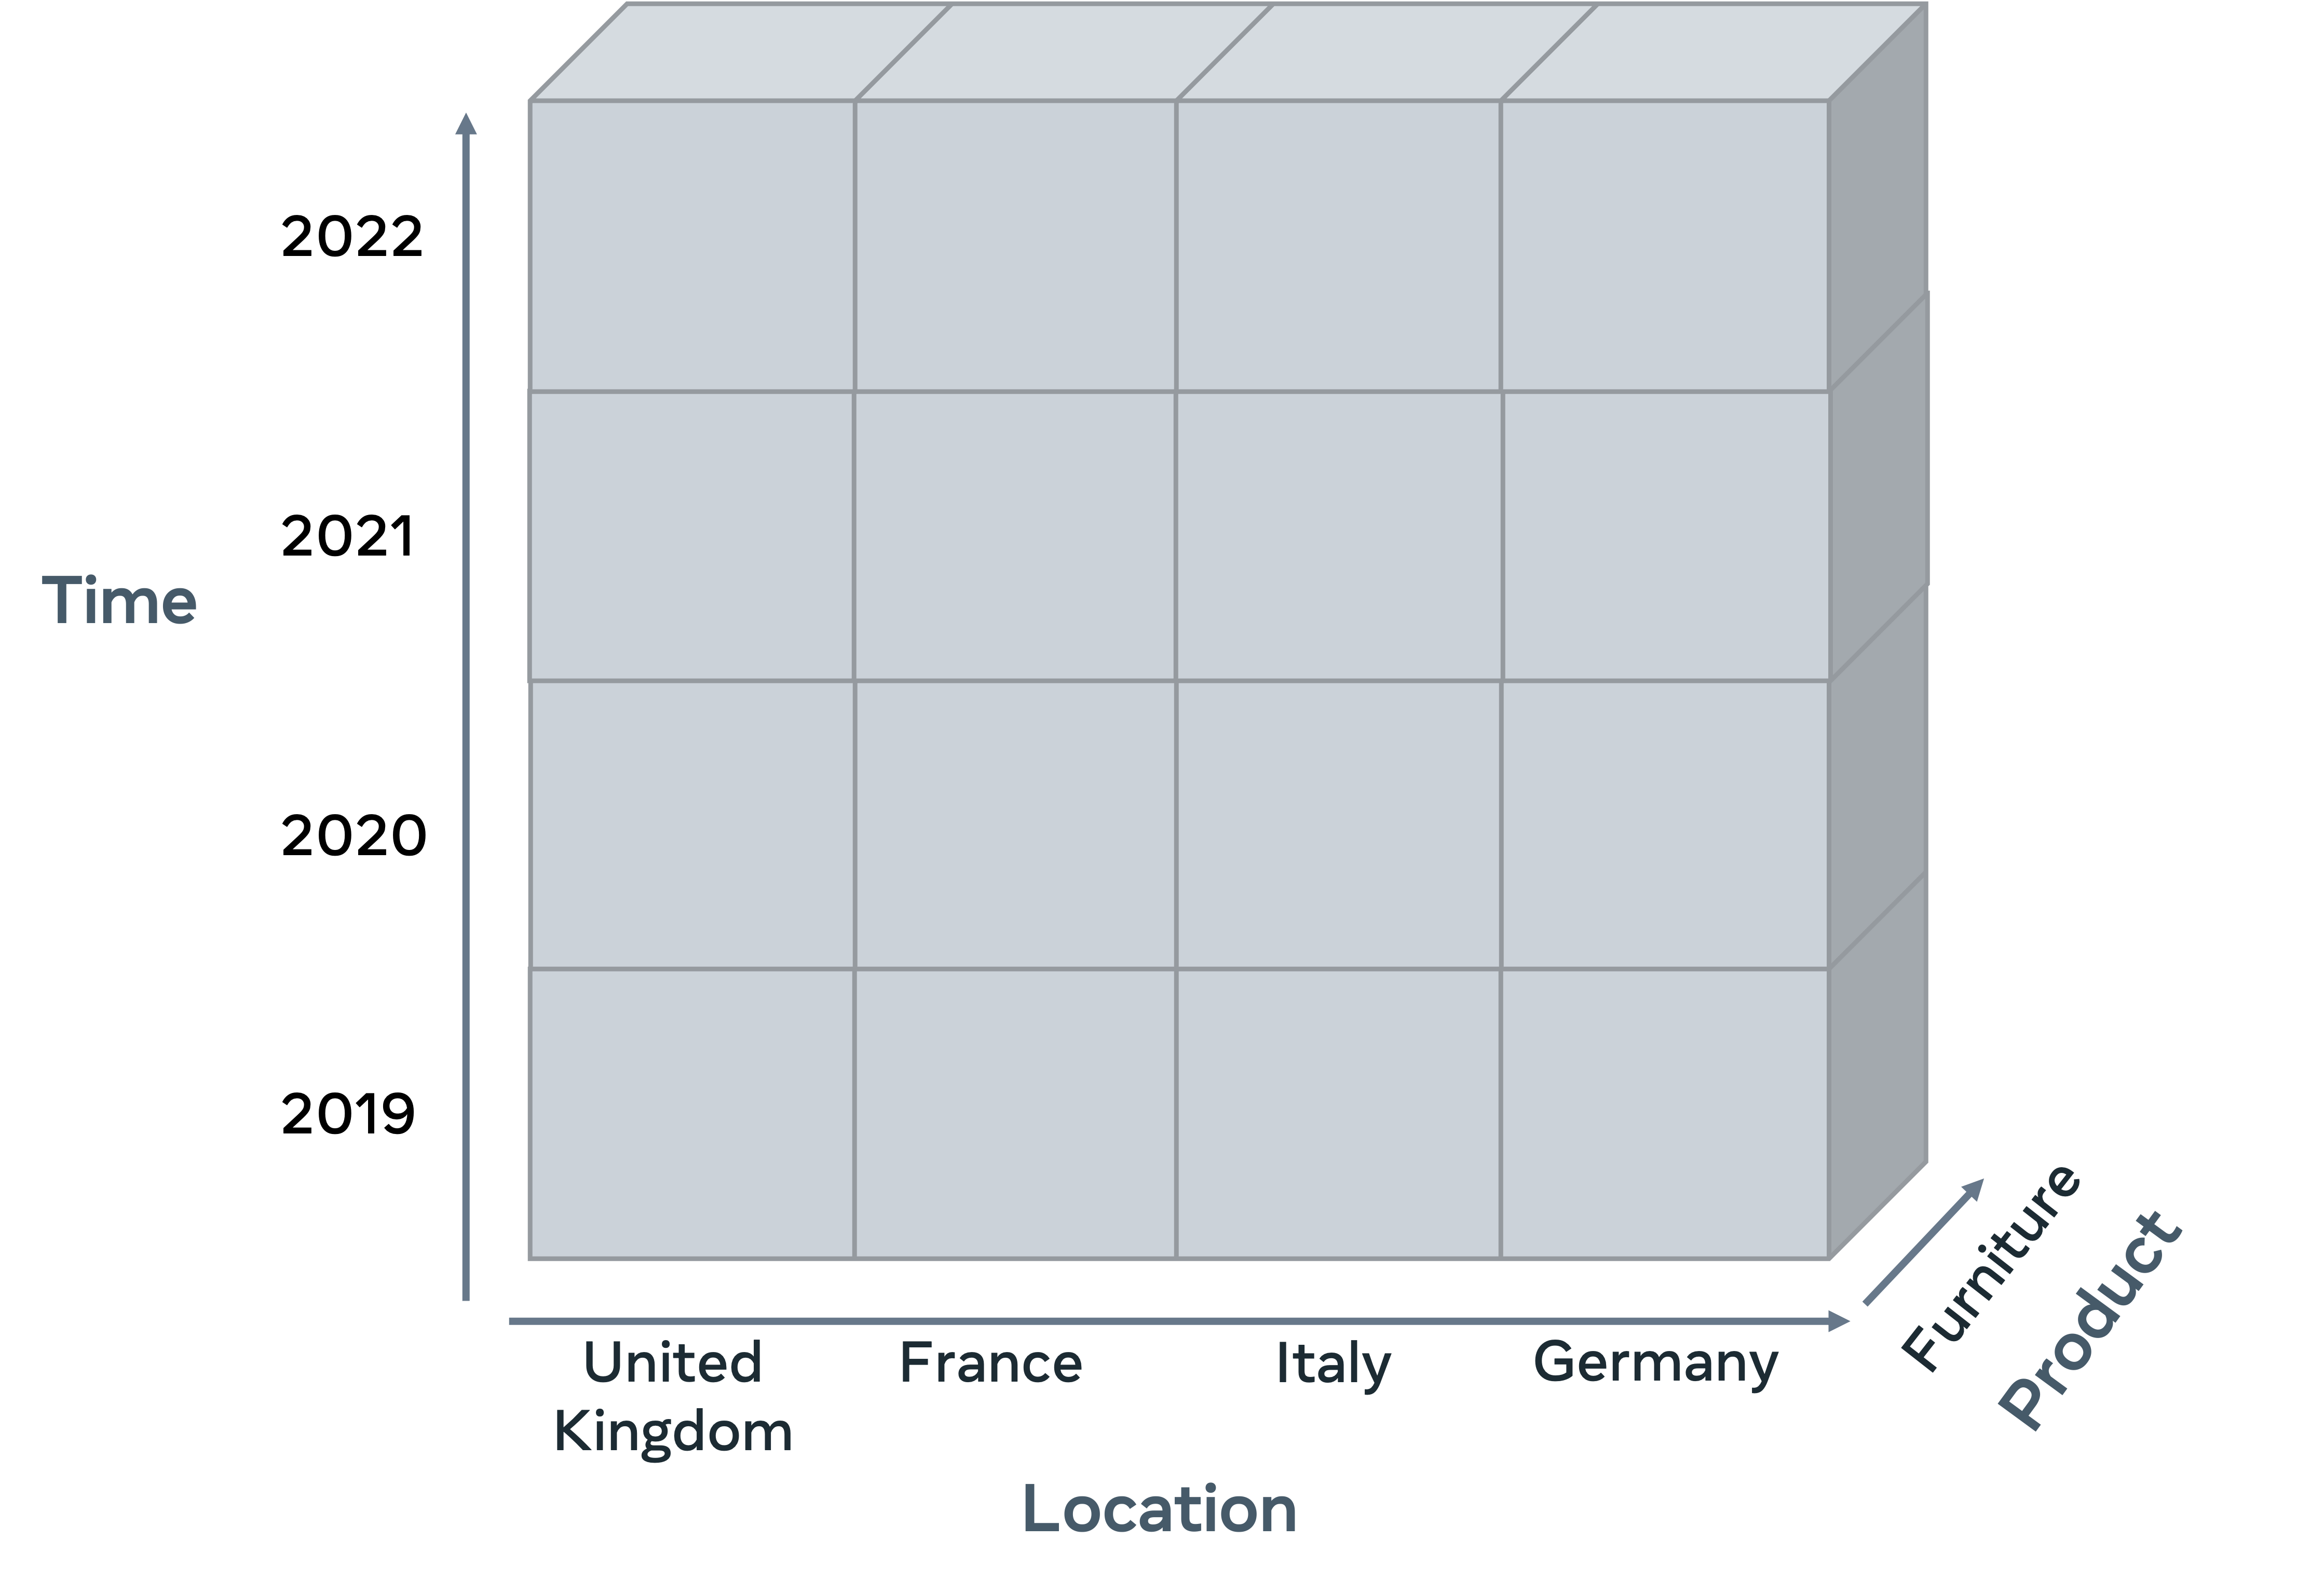
\includegraphics[width=0.8\textwidth]{./Picts/slice.png}
    \caption{}
\end{figure}

Grafik di bawah ini menunjukkan bagaimana operasi slice digunakan untuk menjawab pertanyaan: “Bagaimana kinerja penjualan kategori furnitur selama empat tahun terakhir di setiap negara?”
\begin{figure}[H]
    \centering
    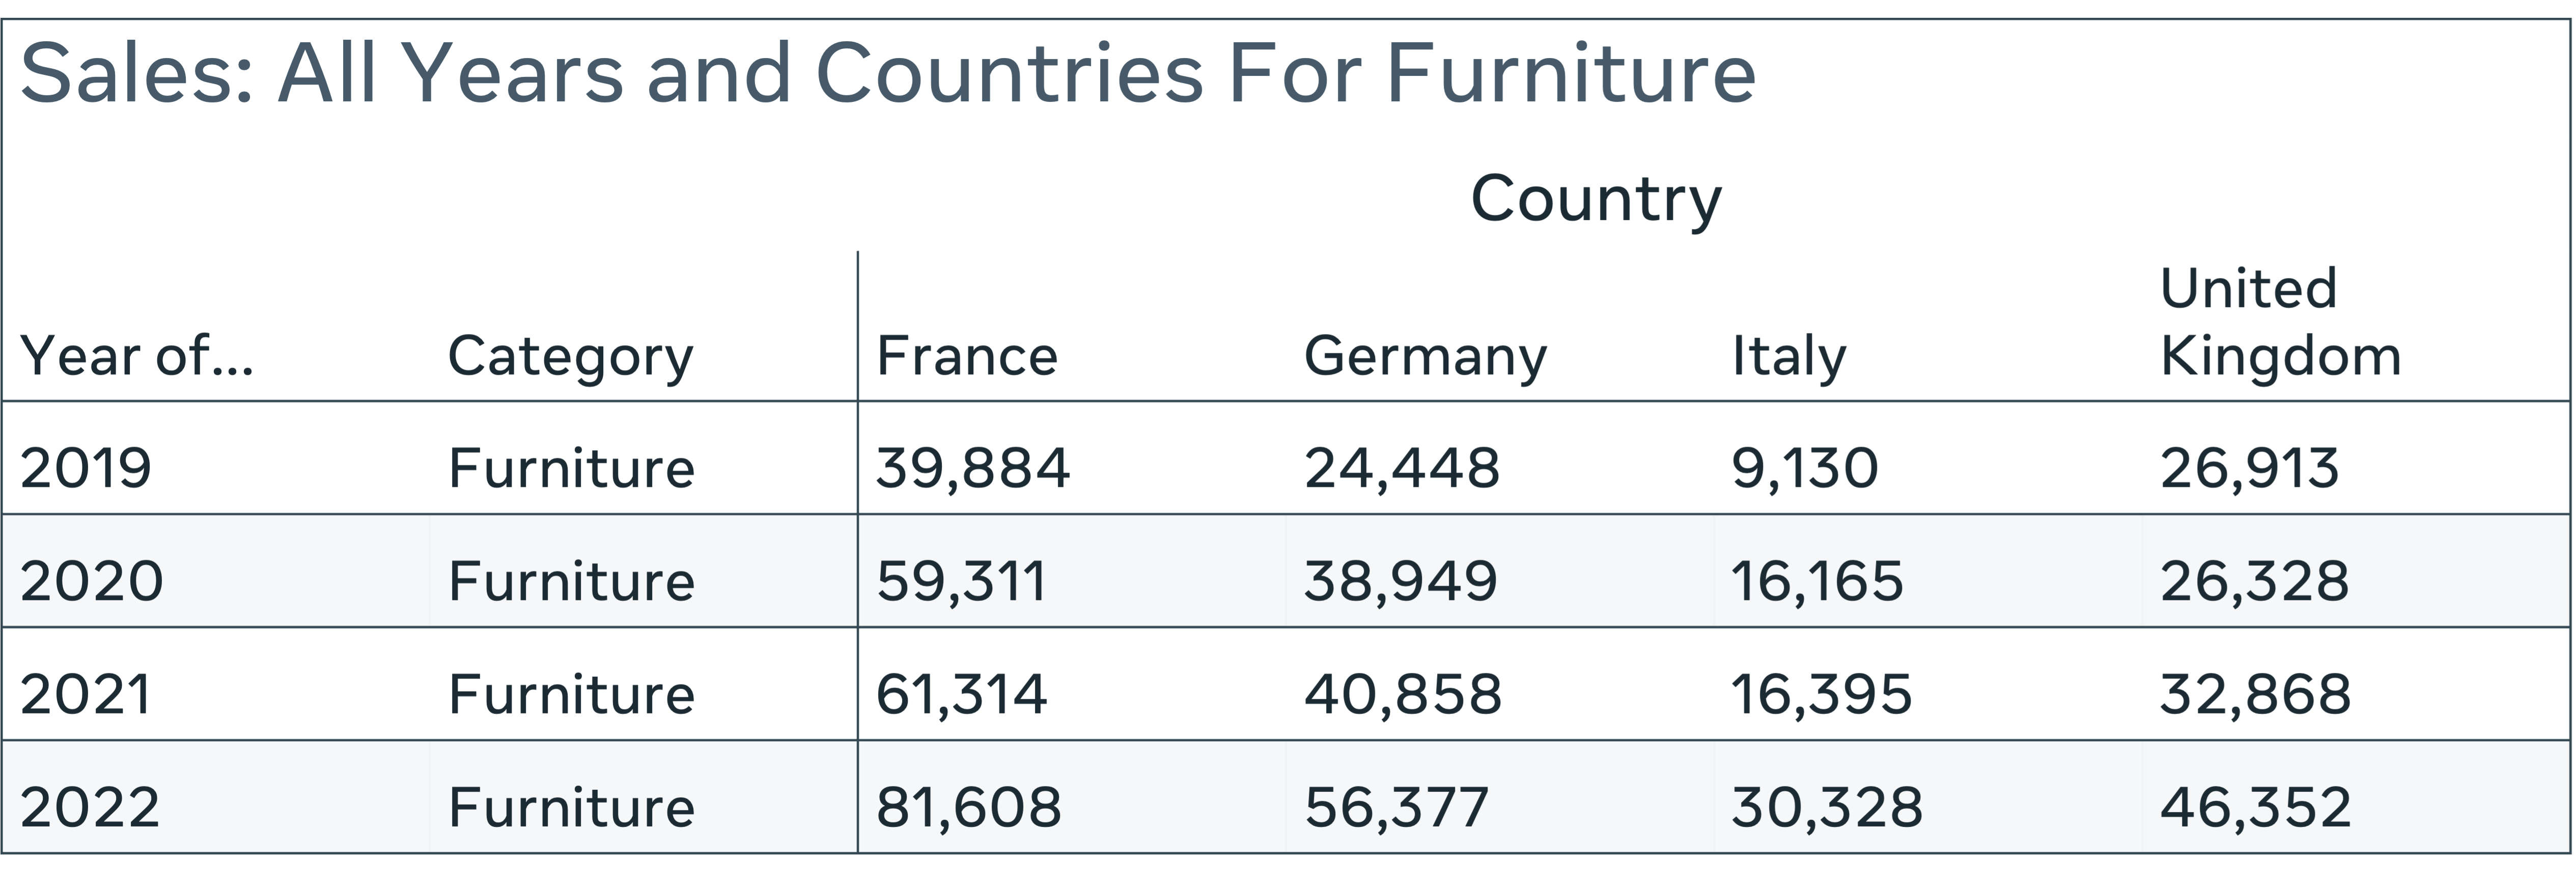
\includegraphics[width=0.8\textwidth]{./Picts/sliceetable.png}
    \caption{}
\end{figure}

\paragraph{Pivot}

Operasi Pivot memberikan tampilan alternatif data dengan memutar sumbu kubus. Misalnya, kubus berikut memutar dimensi Lokasi dan Waktu.
\begin{figure}[H]
    \centering
    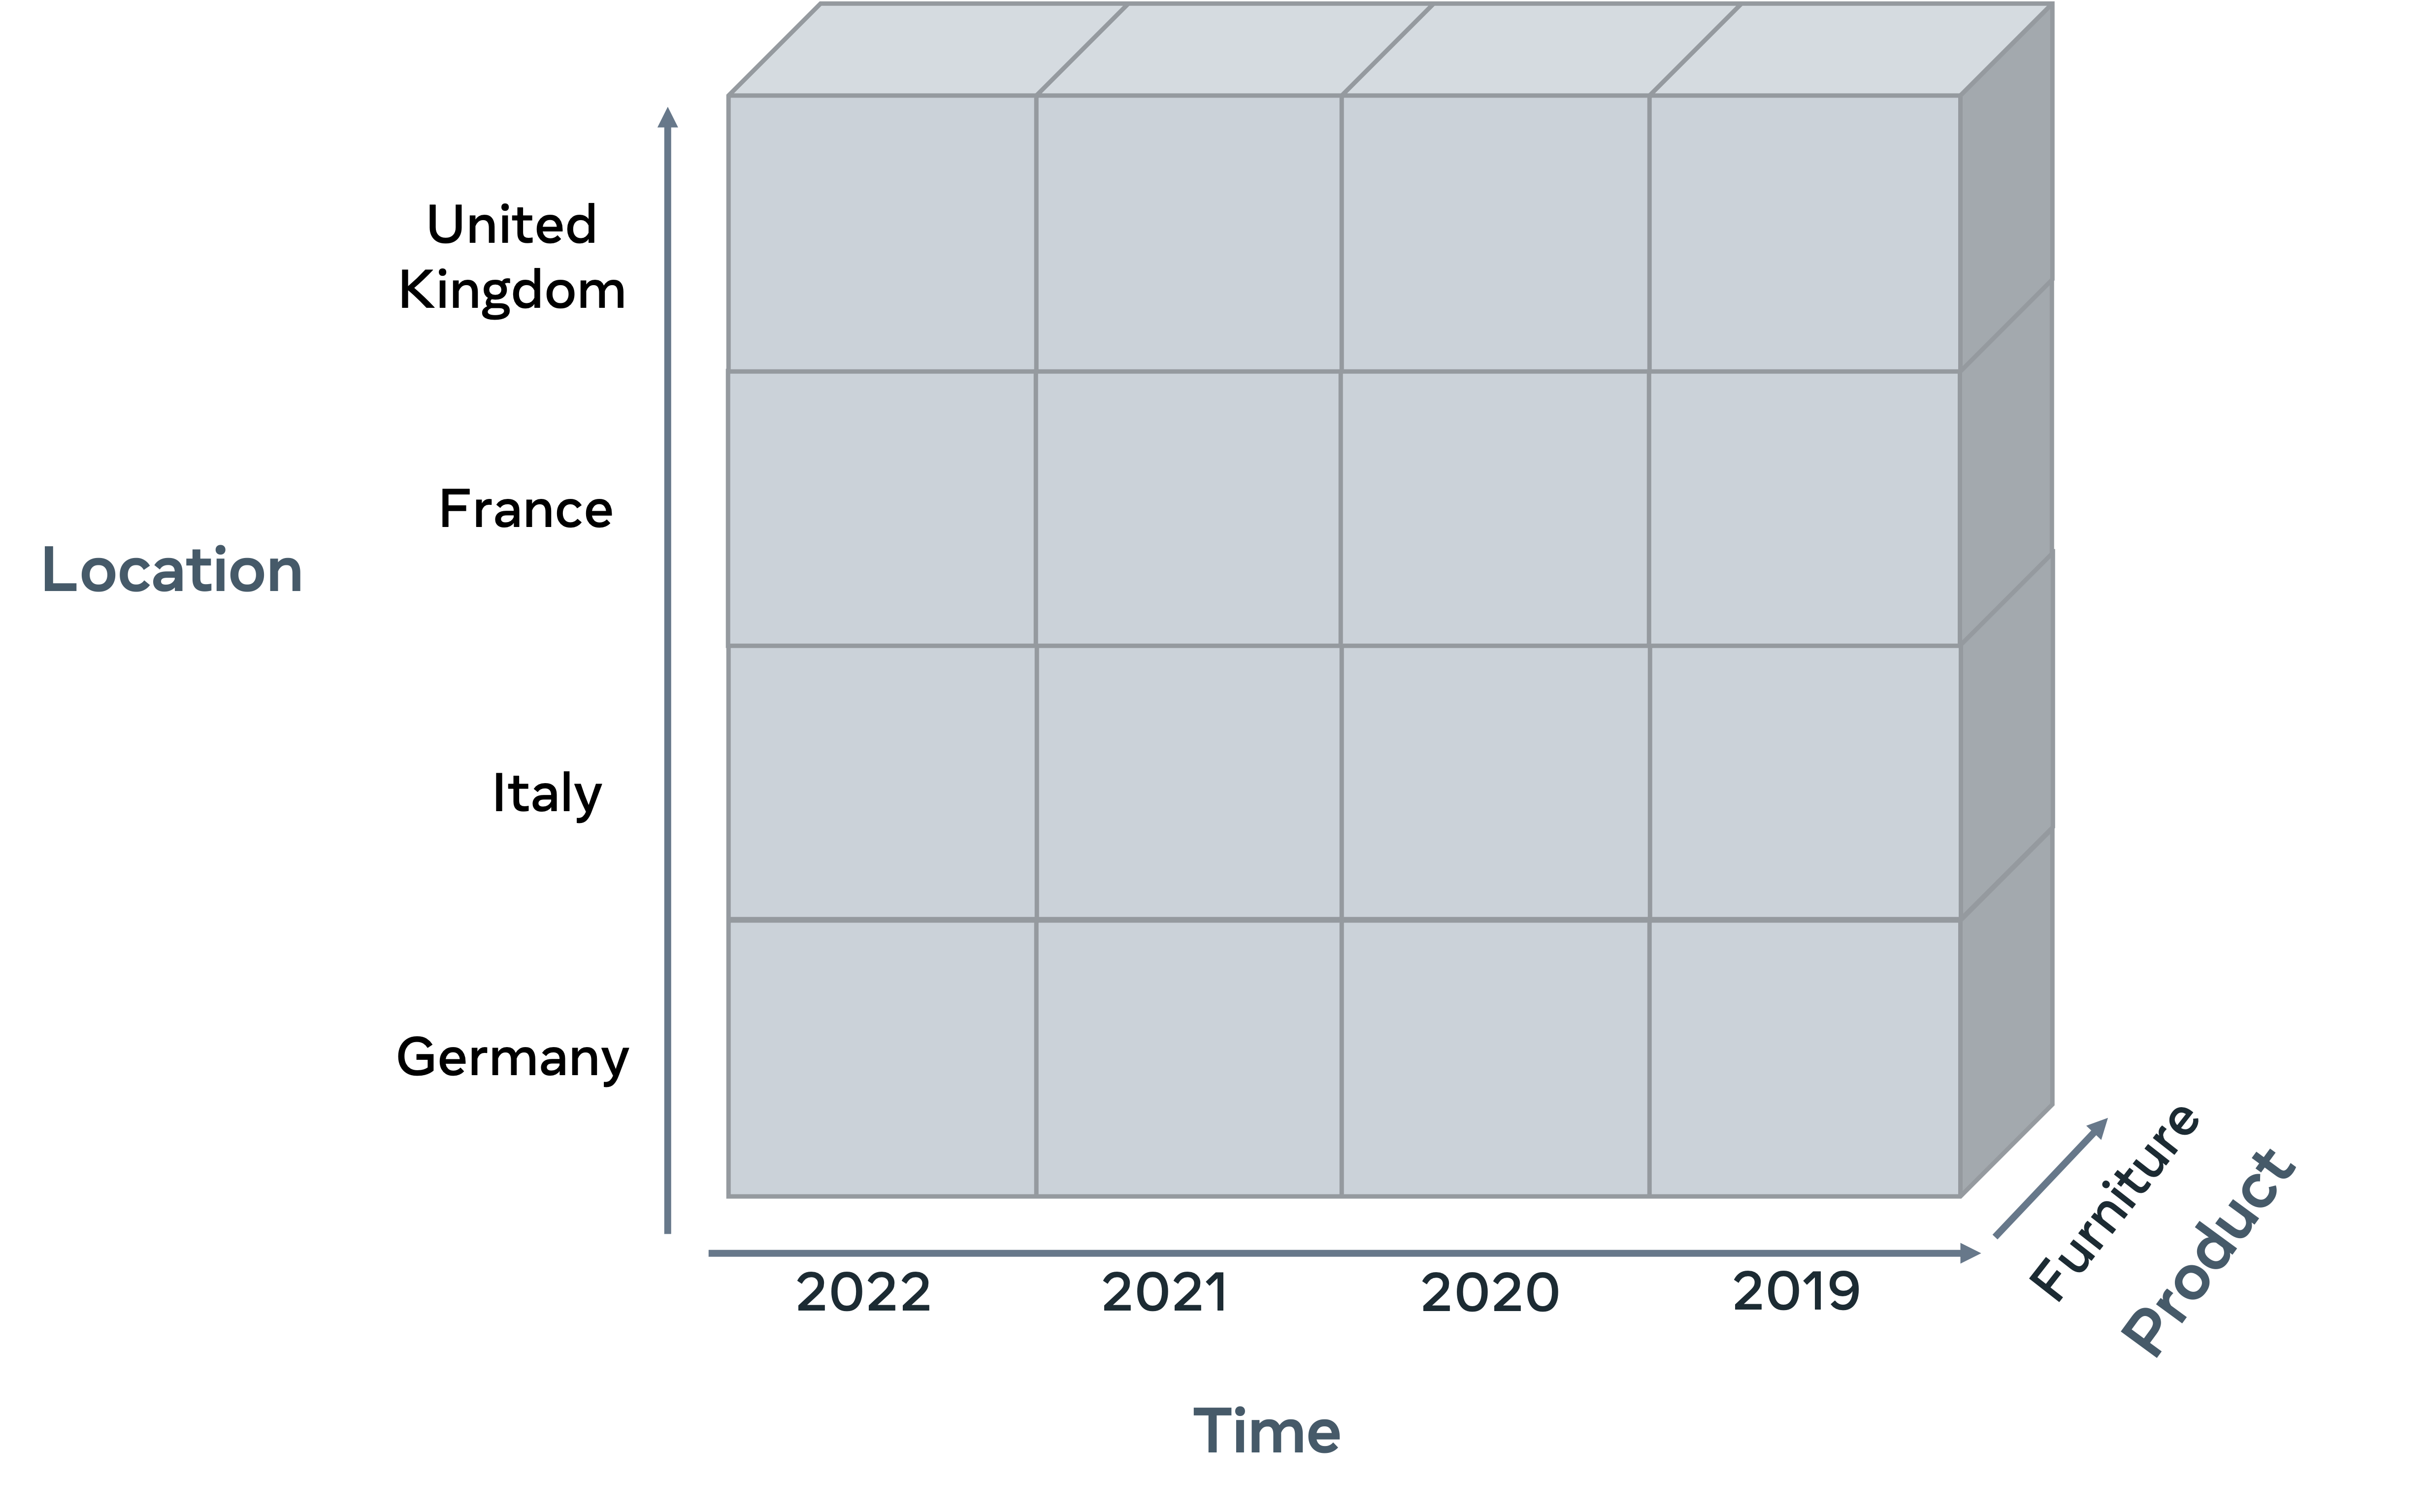
\includegraphics[width=0.8\textwidth]{./Picts/pivot.png}
    \caption{}
\end{figure}
Data pada grafik sebelumnya (Slice) kini ditampilkan secara berbeda. Dimensi Lokasi dan Waktu telah ditukar. Data Negara kini ditampilkan pada kolom pertama, sedangkan data Tahun ditampilkan pada baris, seperti yang ditunjukkan di bawah ini.
\begin{figure}[H]
    \centering
    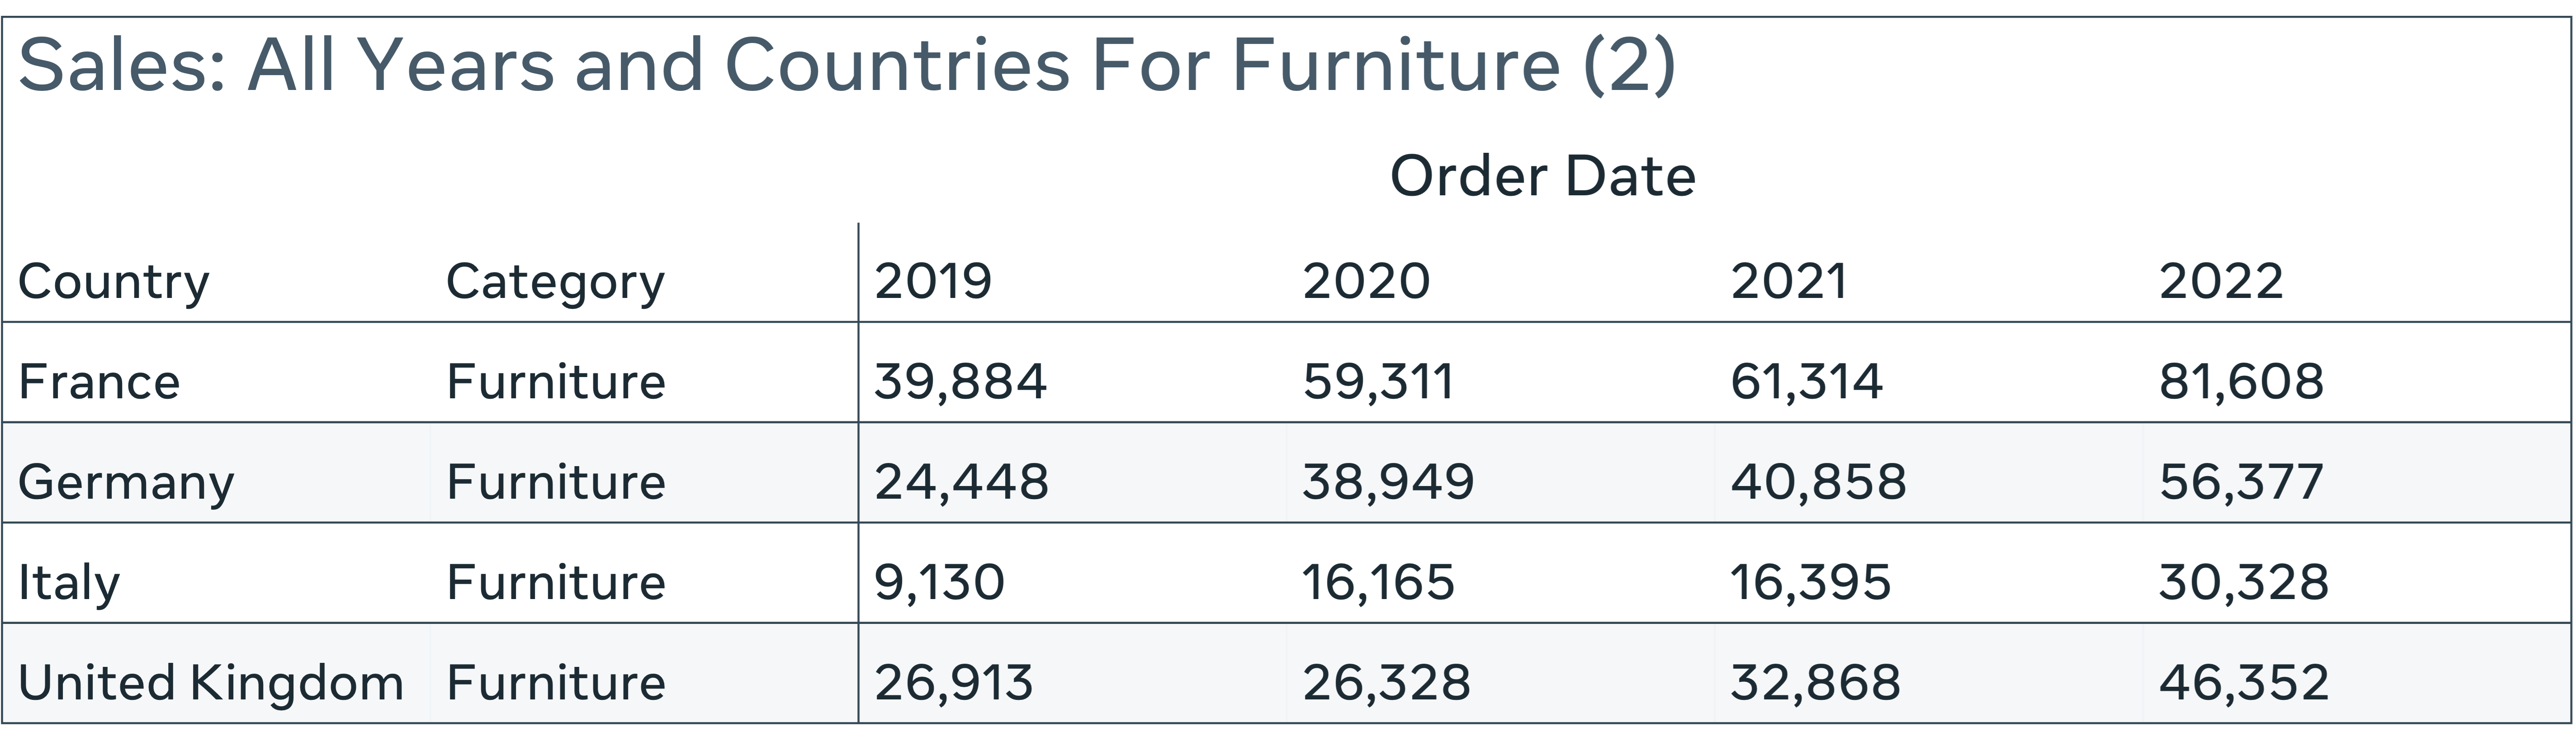
\includegraphics[width=0.8\textwidth]{./Picts/pivottabel.png}
    \caption{}
\end{figure}

\paragraph{Dice}

Operasi dadu menyoroti dua atau lebih subdimensi dari kubus seperti yang ditunjukkan di bawah ini.
\begin{figure}[H]
    \centering
    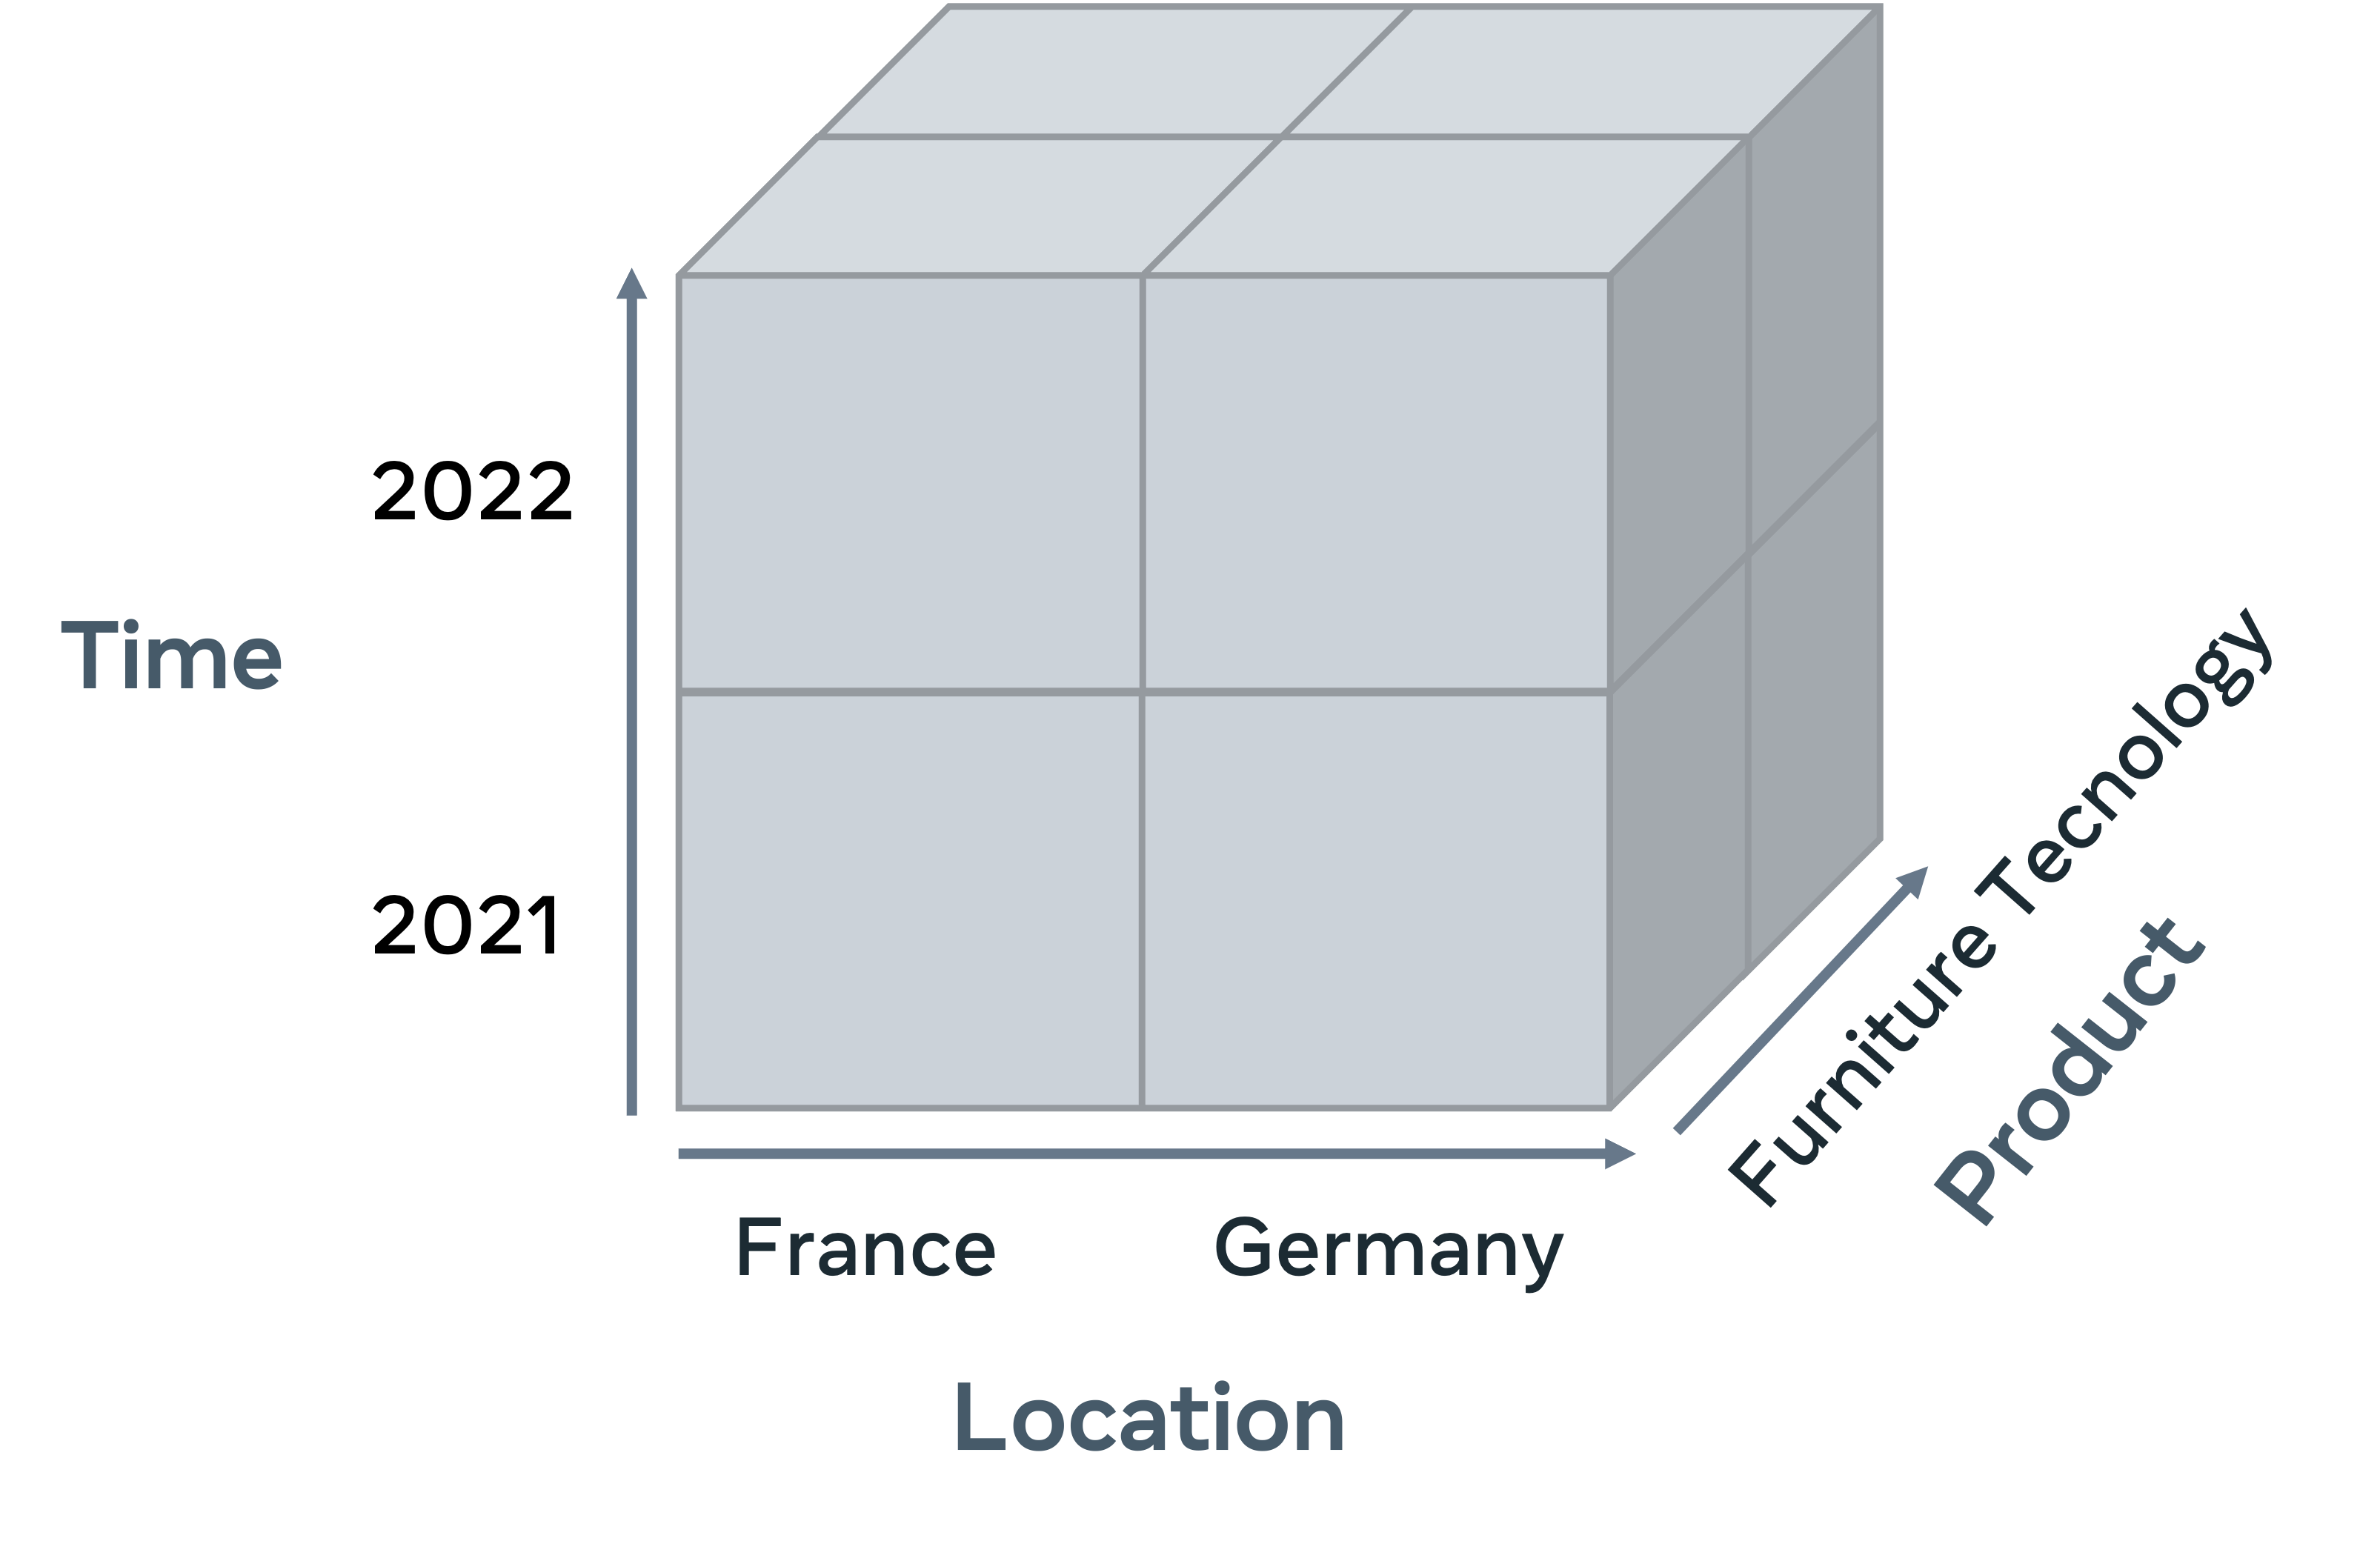
\includegraphics[width=0.8\textwidth]{./Picts/dice.png}
    \caption{}
\end{figure}

Grafik berikut menunjukkan bagaimana operasi dadu digunakan untuk menjawab pertanyaan: “Bagaimana kinerja penjualan produk furnitur dan teknologi selama dua tahun terakhir di Prancis dan Jerman?”
\begin{figure}[H]
    \centering
    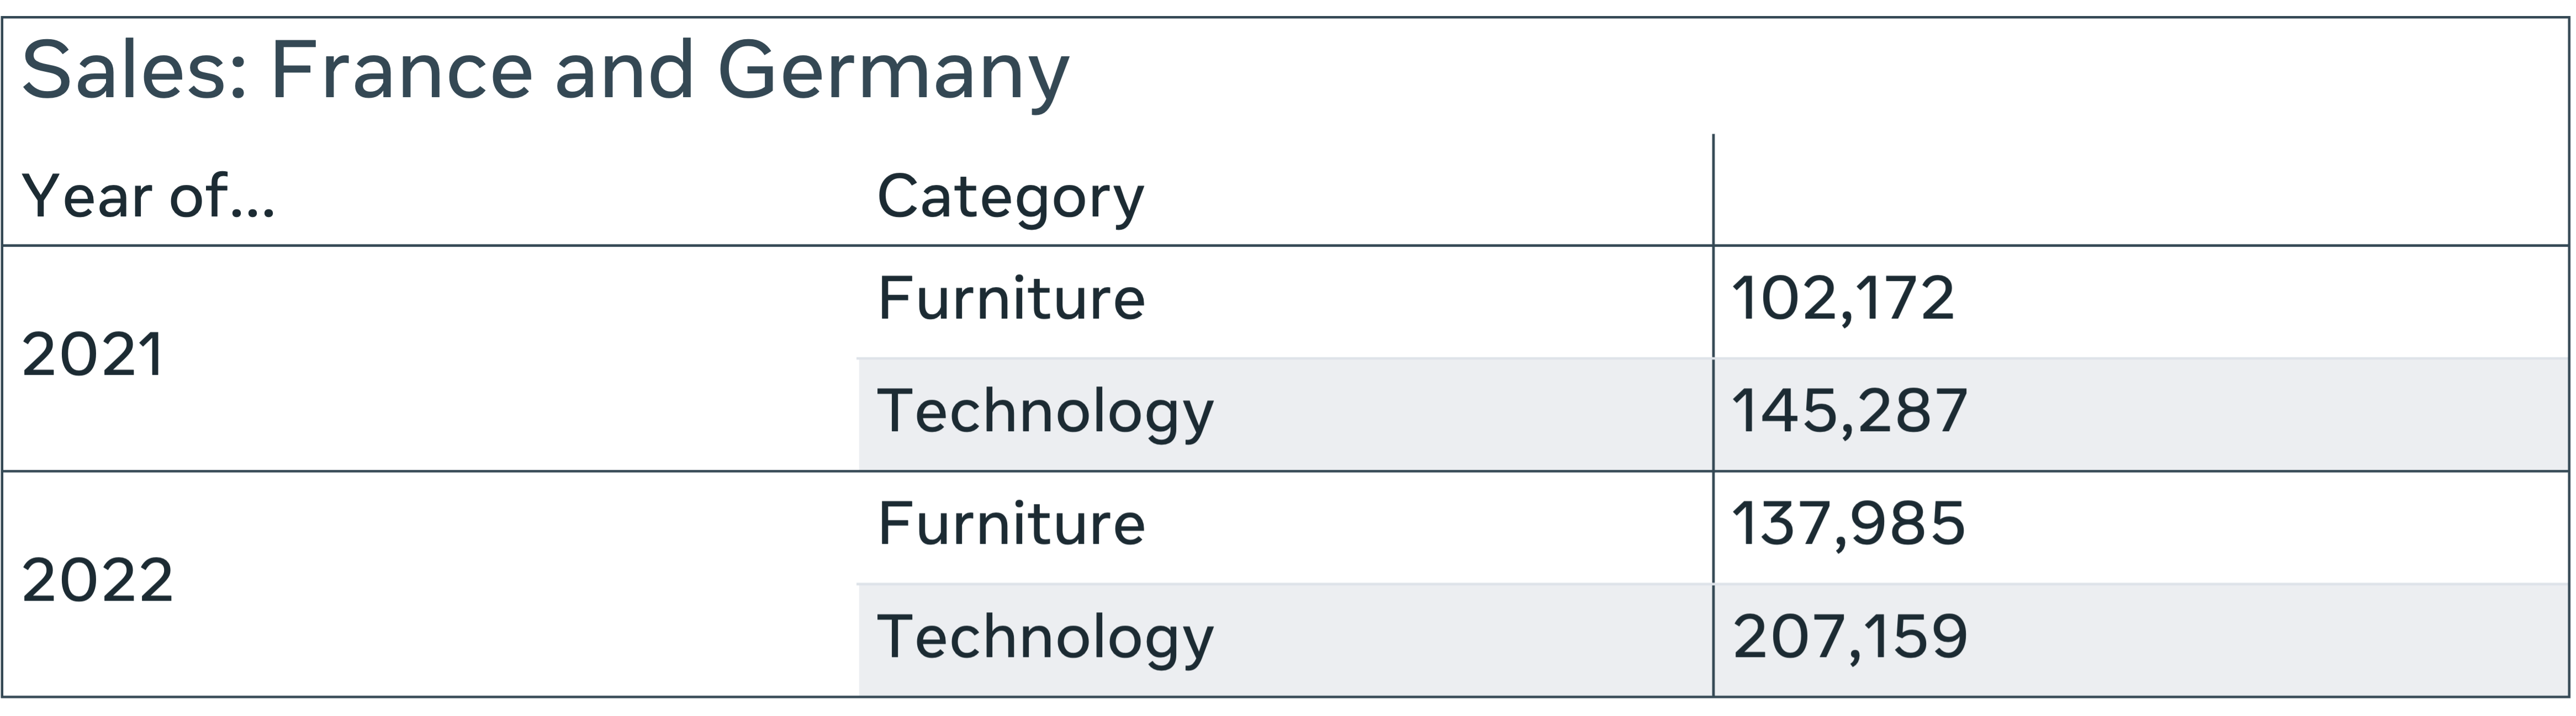
\includegraphics[width=0.8\textwidth]{./Picts/dicetable.png}
    \caption{}
\end{figure}

\paragraph{Drill-down and roll-up}

Model kubus multidimensi juga mendukung struktur data hierarkis. Hal ini memungkinkan Anda untuk melakukan drill down ke area data yang lebih spesifik atau roll-up untuk berpindah ke tingkat data yang lebih tinggi. Grafik berikut, misalnya, menggunakan operasi drill down untuk menampilkan data dalam kuartal daripada tahun.
\begin{figure}[H]
    \centering
    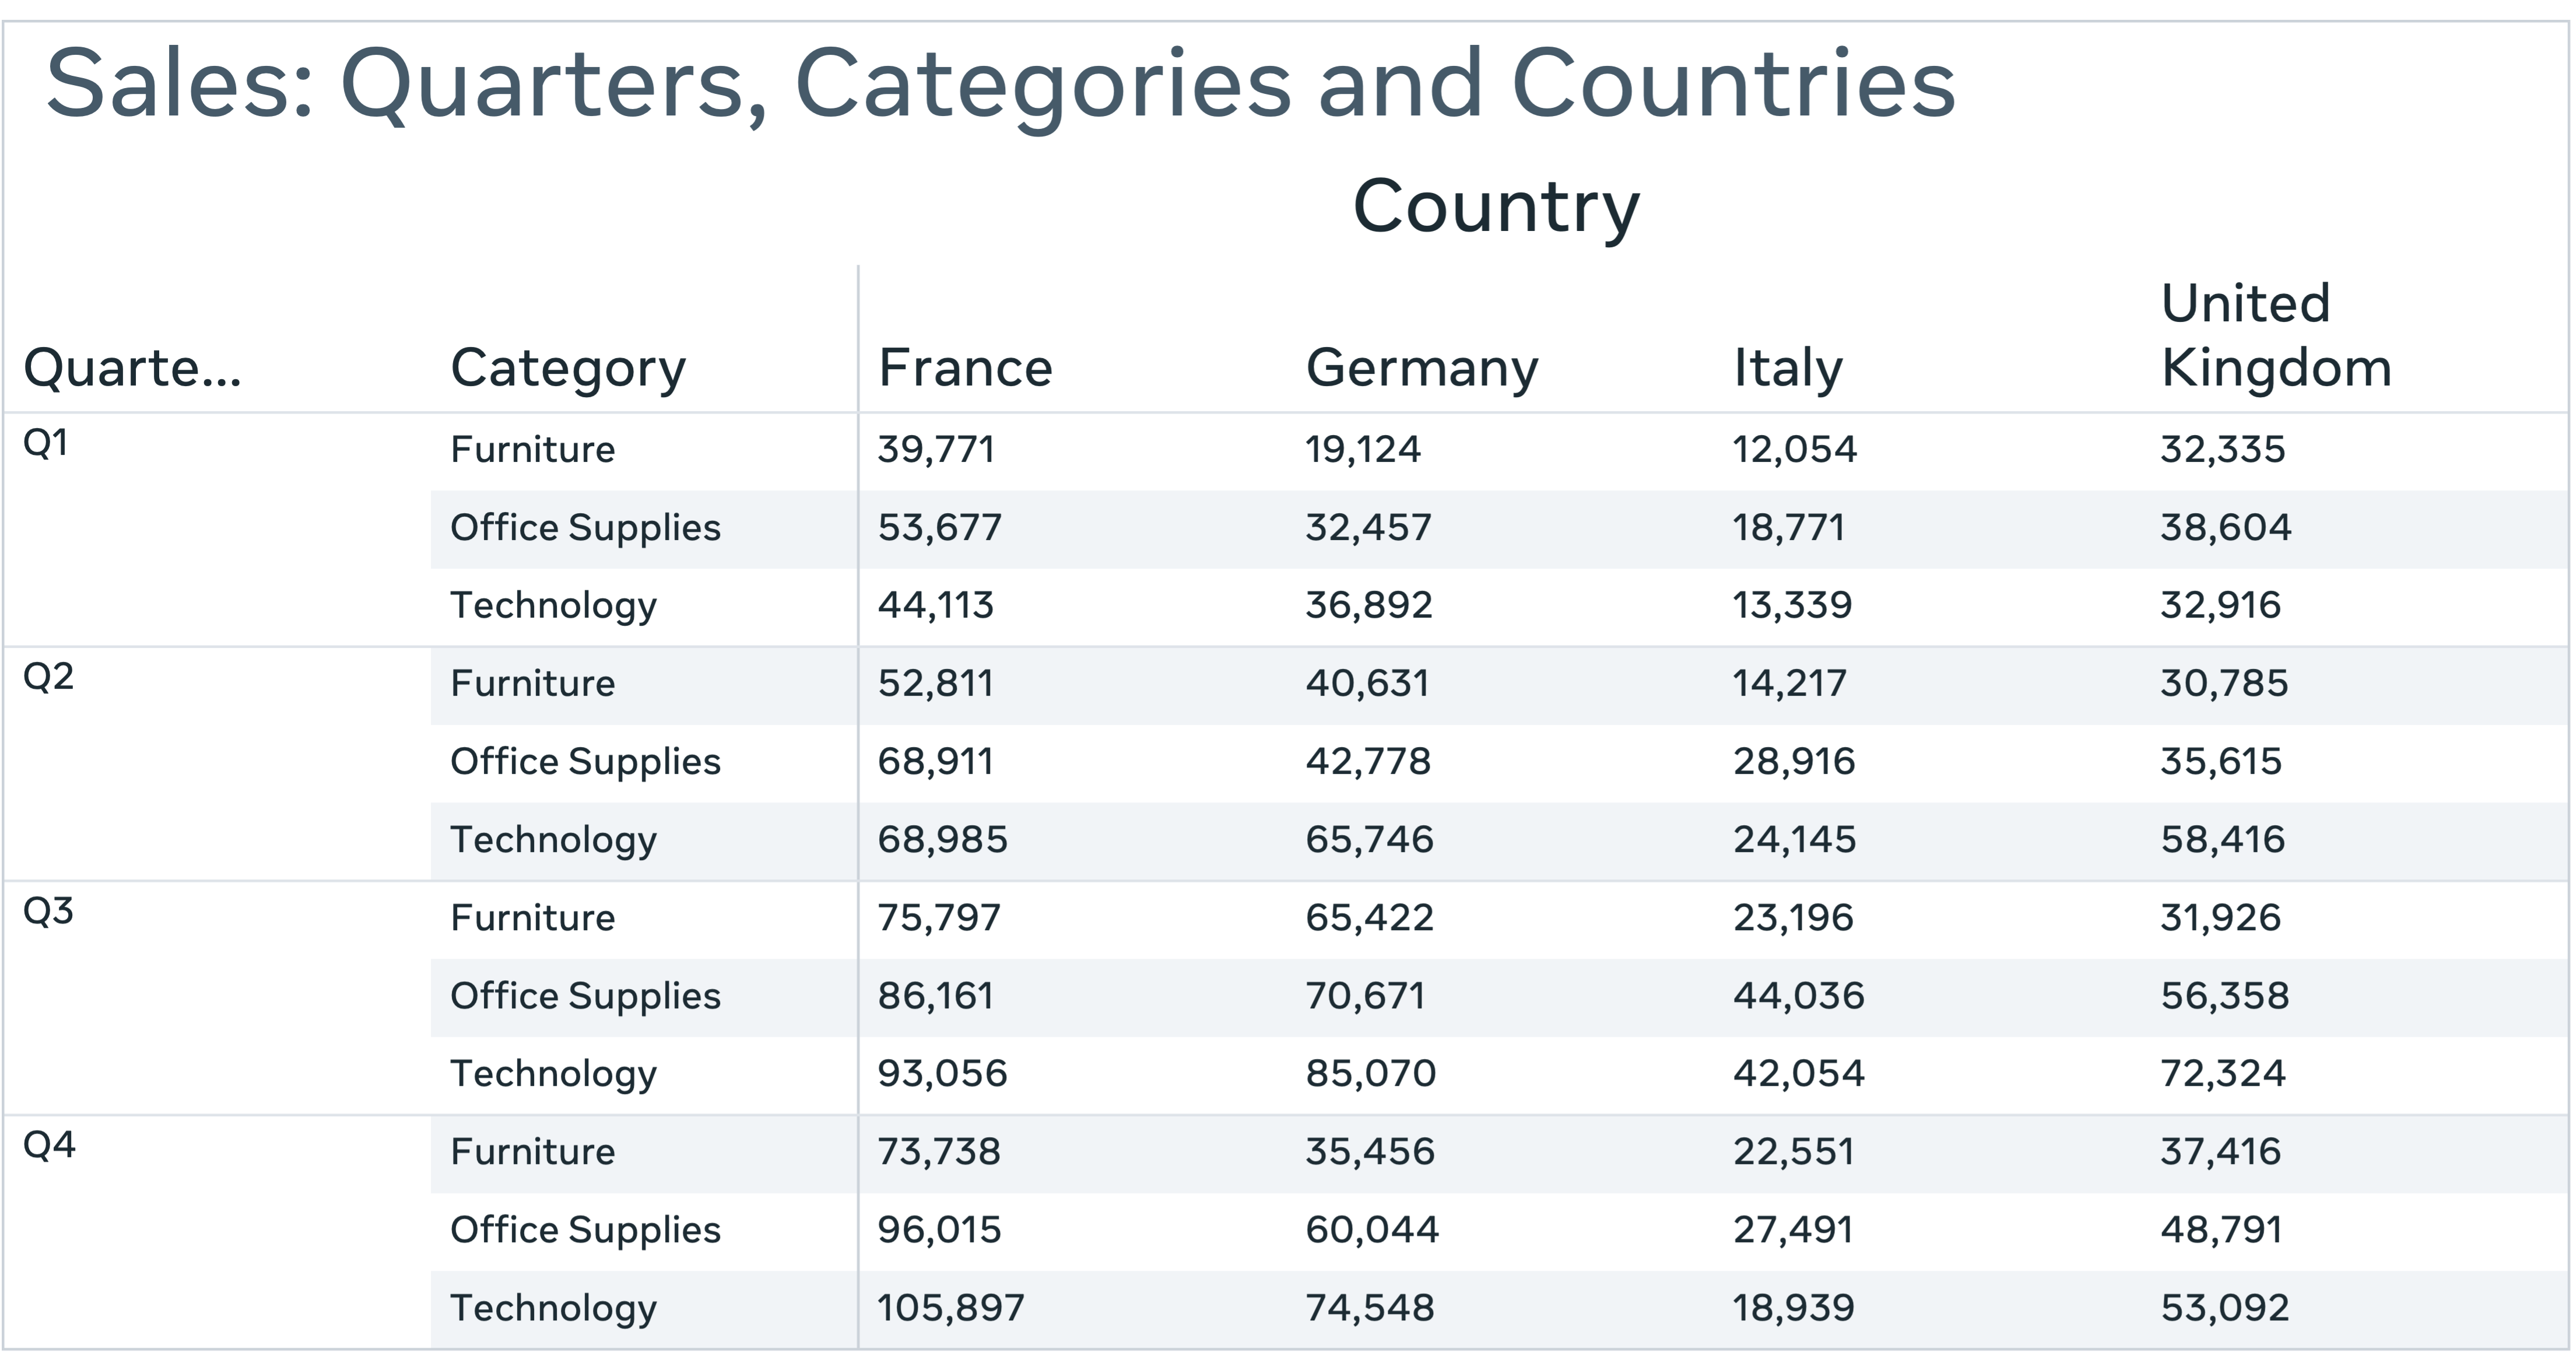
\includegraphics[width=0.8\textwidth]{./Picts/drillnroll.png}
    \caption{}
\end{figure}

\subsection{Tujuan Model Data Dimensional}
Proses membangun model data dimensional menggunakan pendekatan yang dikenal sebagai Kimball's dimensional data modeling
\begin{itemize}
    \item Model data dimensional digunakan untuk memahami aspek tertentu dari bisnis dan menyelesaikan masalah spesifik.
    \item Proses ini melibatkan empat langkah kunci yang harus diambil untuk membangun model data dimensional.
\end{itemize}

\subsection{Empat Langkah Kunci}
\begin{itemize}
    \item Business Process (Proses Bisnis)

          Langkah pertama adalah memilih proses bisnis yang akan dianalisis. Contohnya, Global Super Store memilih untuk menganalisis aktivitas penjualan mereka.

    \item Grain (Grain)

          Setelah memilih proses, langkah berikutnya adalah menentukan tingkat detail yang diperlukan, yang disebut grain. Misalnya, Global Super Store perlu menganalisis data penjualan baik secara tahunan maupun harian.

    \item Dimensions (Dimensi)

          Dalam langkah ini, Anda memilih dimensi yang relevan untuk analisis. Global Super Store perlu menganalisis data penjualan dalam konteks produk, pelanggan, waktu, dan lokasi.

    \item Facts (Fakta)
          Langkah terakhir adalah menentukan apa yang ingin diukur. Anda perlu memilih ukuran yang berisi data numerik untuk mengisi tabel fakta. Misalnya, Global Super Store ingin mengeksplorasi fakta penjualan menggunakan tabel dimensi lokasi, produk, dan waktu.
\end{itemize}

\subsection{Membuat Skema}
Setelah menentukan proses bisnis, grain, dimensi, dan fakta, Anda dapat membuat skema. Global Super Store dapat mengatur dimensi dan ukuran mereka dalam skema bintang (star schema) untuk menganalisis kinerja aktivitas penjualan mereka.

\newpage

\section{Advanced Data Analytics}
\subsection{Dasar-dasar Analisis Data}
\begin{itemize}
    \item Analisis Data: Proses menganalisis data untuk mendapatkan informasi yang berguna dan wawasan yang berharga.
    \item Data Analytics Tools: Alat yang digunakan untuk melakukan analisis data.
\end{itemize}

\subsection{Jenis-jenis Analisis Data}
\begin{itemize}
    \item Descriptive Data Analysis: Menyajikan data dalam format deskriptif untuk memberikan gambaran umum.
    \item Exploratory Data Analysis: Digunakan untuk menetapkan hubungan antara variabel yang berbeda.
    \item Inferential Data Analysis: Fokus pada sampel kecil data untuk membuat inferensi tentang populasi yang lebih besar.
    \item Predictive Data Analysis: Mengidentifikasi pola dalam data untuk memprediksi kinerja di masa depan.
    \item Causal Data Analysis: Meneliti hubungan sebab-akibat antara variabel.
\end{itemize}

\subsection{Tipe Data dan Pengukuran}
\begin{itemize}
    \item Quantitative Data: Data numerik yang dapat dihitung, seperti jumlah rata-rata pelanggan yang melakukan pembelian setiap hari.
    \item Qualitative Data: Data non-numerik yang bersifat deskriptif, seperti nama kategori produk.
\end{itemize}

\subsection{Skala Pengukuran}
\begin{itemize}
    \item Nominal Scale:

          Menggambarkan data non-numerik yang bersifat deskriptif, seperti mengidentifikasi produk (contoh: kursi, meja).

          Ini adalah skala yang digunakan untuk mengidentifikasi atau memberi nama pada kategori tanpa urutan. Contohnya, jika kita memiliki kategori produk seperti "meja", "kursi", dan "lemari", kita hanya memberi label pada masing-masing tanpa ada peringkat. Jadi, kamu benar bahwa ini adalah nama identifier.

    \item Ordinal Scale:

          Data kualitatif yang diurutkan dalam urutan tertentu tanpa kriteria yang jelas untuk perbedaan antar elemen (contoh: peringkat kualitas produk).

          Ini adalah skala yang memberikan peringkat pada data, tetapi tidak menunjukkan seberapa besar perbedaan antara peringkat tersebut. Misalnya, jika kita memberi rating pada produk dari 1 hingga 5, kita tahu bahwa 5 lebih baik dari 4, tetapi kita tidak tahu seberapa besar perbedaan antara keduanya.

    \item Interval Scale:

          Memiliki sifat dari skala nominal dan ordinal, di mana perbedaan antara titik data dapat diidentifikasi (contoh: umpan balik produk dari -10 hingga 10).

          Ini adalah skala yang menunjukkan perbedaan yang sama antara nilai-nilai, tetapi tidak memiliki titik nol yang absolut. Contohnya adalah suhu dalam derajat Celsius. Kita bisa mengatakan bahwa 20°C lebih panas dari 10°C, dan perbedaan antara keduanya adalah 10 derajat. Namun, 0°C tidak berarti "tidak ada suhu". Jadi, ini adalah skala yang lebih kompleks karena kita bisa melakukan operasi matematika seperti penjumlahan dan pengurangan, tetapi tidak bisa melakukan perkalian atau pembagian.

    \item Ratio Scale:

          Data kuantitatif yang memiliki nilai absolut nol dan mencakup sifat dari ketiga skala sebelumnya (contoh: berat produk, seperti meja kecil 20 kg, meja sedang 40 kg, meja besar 60 kg).

          Ini adalah skala yang memiliki semua sifat dari skala nominal, ordinal, dan interval, tetapi juga memiliki titik nol yang absolut. Contohnya adalah berat atau tinggi. Jika sesuatu memiliki berat 0 kg, itu berarti tidak ada berat sama sekali. Kita bisa melakukan semua operasi matematika di sini, termasuk perkalian dan pembagian. Mencakup ukuran fisik seperti massa, tinggi, dan volume.
\end{itemize}

\subsection{Data Mining dan Machine Learning}
\begin{itemize}
    \item Data Mining: Proses mendeteksi pola dalam data untuk mendapatkan wawasan dan membuat prediksi. Contoh: Global Super Store menggunakan data mining untuk mengidentifikasi pola pembelian produk, seperti pelanggan yang membeli meja juga membeli kursi.
    \item Machine Learning: Proses mengajarkan komputer untuk belajar dan membuat prediksi. Ada dua metode utama:
          \begin{itemize}
              \item Supervised Machine Learning: Mengklasifikasikan data berdasarkan label yang diberikan. Contoh: Mengelompokkan gambar kursi dan meja dengan label CH dan DK.
              \item Unsupervised Machine Learning: Mengklasifikasikan data berdasarkan karakteristik yang sama tanpa label. Contoh: Mengelompokkan gambar objek berdasarkan bentuk.
          \end{itemize}
\end{itemize}

\subsection{Model Data Mining}
\begin{itemize}
    \item Classification Analysis: Model yang mengelompokkan item data ke dalam kategori. Contoh: Pelanggan yang membeli produk kantor berharga rendah dapat diklasifikasikan sebagai pelanggan dengan anggaran rendah.

          Kita mengelompokkan data ke dalam kategori yang sudah ditentukan sebelumnya. Misalnya, jika kita memiliki gambar-gambar produk, kita bisa mengklasifikasikannya menjadi kategori seperti "meja" atau "kursi". Dalam hal ini, kita sudah tahu label untuk setiap kategori, dan kemudian Machine Learning untuk mengenali dan mengelompokkan data berdasarkan label tersebut.
    \item Association Rule: Model yang mengidentifikasi hubungan antara elemen data. Contoh: Pelanggan yang membeli ponsel juga membeli charger dan baterai.
    \item Outlier Detection: Model yang mendeteksi data yang tidak biasa dalam dataset. Contoh: Pelanggan yang biasanya membeli produk murah tiba-tiba membeli produk mahal.
    \item Clustering Analysis: Model yang mencari kesamaan dalam dataset dan memisahkan data menjadi kelompok berdasarkan kesamaan. Contoh: Mengelompokkan pelanggan berdasarkan perilaku navigasi di toko online.

          Kita mengelompokkan data tanpa menggunakan label yang sudah ada. Ini berarti kita mencari pola atau kesamaan dalam data untuk mengelompokkannya. Misalnya, jika kita memiliki data pelanggan, clustering dapat membantu kita menemukan kelompok pelanggan yang memiliki perilaku belanja yang mirip, meskipun kita tidak tahu sebelumnya kategori apa yang ada.
    \item Regression Analysis: Model yang mempertimbangkan faktor-faktor yang mempengaruhi data dan menentukan hubungan antara faktor-faktor tersebut. Contoh: Diskon produk yang meningkatkan penjualan.
\end{itemize}

\subsection{Nilai dari Wawasan Data dalam Bisnis}
\subsubsection{Overview}
Organisasi mengumpulkan banyak data dan menyimpannya dalam berbagai jenis basis data. Data ini merupakan aset penting yang dapat digunakan untuk menganalisis aktivitas dan kinerja bisnis. Namun, untuk mendapatkan manfaat maksimal dari data ini, Anda perlu mengelolanya dengan baik agar dapat diubah menjadi sumber daya yang berharga.

Demikian pula, data dapat diakses, diekstraksi, disempurnakan, dan dianalisis untuk menemukan hubungan antara data yang ada guna menciptakan wawasan yang membantu pengambil keputusan dalam merencanakan aktivitas bisnis, meningkatkan layanan, mengurangi biaya, meminimalkan risiko, dan meningkatkan pendapatan.

Analisis data tidak hanya berhenti pada menganalisis data untuk menggambarkannya (seperti berapa banyak pelanggan yang melakukan pemesanan, atau nilai penjualan total). Ini hanyalah fase pertama dalam analisis data. Analisis data memproses data untuk mengevaluasi probabilitas masa depan, mengidentifikasi masalah, menilai risiko, dan memprediksi peluang masa depan.

Untuk melakukan analisis data yang tepat, Anda harus melakukan berbagai jenis analisis data untuk mengidentifikasi model, pola, paradigma, dan tren. Hal ini kemudian membantu Anda memahami kinerja bisnis secara mendalam dan memprediksi hasil masa depan dari aktivitas bisnis. Anda bahkan mungkin mendapatkan rekomendasi untuk rencana terbaik dan langkah-langkah yang harus diambil.

\subsubsection{Keuntungan dari Data Analitik dalam Bisnis}

Selama dekade terakhir, analisis data telah memainkan peran penting dalam menentukan cara organisasi menilai risiko dan mencari peluang. Perusahaan besar dan organisasi seperti Amazon, Microsoft, dan Apple telah menginvestasikan miliaran dolar dalam analisis data canggih.

Penting untuk menyadari bahwa cara-cara di mana analisis data dapat dimanfaatkan bergantung pada berbagai faktor seperti kebutuhan bisnis, kondisi pasar, pesaing, dan bidang usaha. Namun demikian, terdapat manfaat umum yang dapat diperoleh dari analisis data terlepas dari ukuran dan jenis bisnis.

Misalnya, analisis data dapat digunakan untuk:
\begin{itemize}
    \item Memberikan wawasan yang terperinci, akurat, dan dapat diandalkan untuk meningkatkan pengambilan keputusan bisnis sehari-hari.
    \item Mengidentifikasi dan memanfaatkan peluang potensial.
    \item Menemukan cara untuk memonetisasi data.
    \item Mengidentifikasi ancaman seperti celah keamanan dan pelanggaran.
    \item Memprediksi dan merespons secara proaktif perubahan dan tantangan di pasar.
    \item Mendapatkan gambaran menyeluruh tentang aktivitas dan operasi bisnis.
    \item Mencegah penipuan.
    \item Dan mengungkap area baru di mana Anda dapat mengurangi biaya bisnis atau pengeluaran dan meningkatkan keuntungan.
\end{itemize}

Penting juga untuk diingat bahwa saat ini bisnis Anda merupakan bagian dari lingkungan Big Data. Lingkungan ini mencakup jumlah data yang sangat besar dan berbagai jenis data kompleks, termasuk data terstruktur, semi-terstruktur, dan tidak terstruktur. Data ini berasal dari berbagai sumber data, seperti basis data OLTP, data komersial, riwayat penelusuran, mesin pencari, dan situs media sosial.

Misalnya, setiap hari Facebook menghasilkan lebih dari 500 terabyte data dari posting, termasuk gambar, komentar, dan video. Demikian pula, Google menghasilkan lebih dari 20 petabyte data setiap hari melalui prosesnya di kluster komputasi besar-besaran. Statistik ini menyoroti pentingnya menggunakan kecerdasan buatan, pembelajaran mesin, dan penambangan data untuk membantu bisnis mengambil keputusan yang didasarkan pada data.

\subsubsection{Teknik Data Analitik}
Ada banyak teknik yang dapat digunakan dalam analisis data untuk memaksimalkan nilai wawasan data. Beberapa teknik yang sering digunakan beserta contoh relevannya tercantum di bawah ini.
\begin{itemize}
    \item Classification technique

          Teknik klasifikasi mengelompokkan item data ke dalam kategori atau kelas, yang memungkinkan Anda memprediksi kelas target dari data Anda. Misalnya, bank menggunakan teknik ini untuk mengidentifikasi pemohon pinjaman dengan risiko kredit rendah, sedang, atau tinggi berdasarkan riwayat peringkat kredit mereka, riwayat pekerjaan, kepemilikan properti, dan sebagainya.

    \item Association rule

          Aturan asosiasi mengidentifikasi hubungan antara elemen data untuk menentukan apakah ada korelasi antara data. Contoh klasik dari aturan asosiasi adalah mengidentifikasi hubungan antara dua produk di toko. Misalnya, banyak pelanggan yang datang ke toko untuk membeli produk tertentu mungkin juga membeli produk terkait lainnya. Oleh karena itu, data menunjukkan bahwa ada hubungan antara kedua produk tersebut. Asosiasi ini mungkin didasarkan pada data yang menunjukkan bahwa 70\% dari total transaksi di toko tersebut melibatkan kedua produk tersebut. Data ini menunjukkan bahwa ada hubungan asosiasi antara kedua produk tersebut.

    \item Outlier detection

          Deteksi outlier digunakan untuk mengidentifikasi data yang tidak biasa dalam suatu kumpulan data. Contoh umum dalam model analitik ini adalah deteksi penipuan kartu kredit. Teknik ini dapat digunakan untuk memeriksa apakah transaksi yang masuk sesuai dengan profil dan perilaku pelanggan. Jika permintaan tidak sesuai dengan profil dan perilaku pelanggan yang ada, maka permintaan tersebut akan ditandai sebagai outlier atau deteksi anomali.

    \item Clustering analysis

          Clustering Analysis mencari kesamaan di dalam sekumpulan data. Jika menemukan kesamaan, maka analisis ini memisahkan data yang terkait ke dalam kelompok-kelompok subset berdasarkan karakteristik bersama mereka.

          Contoh yang baik dari analisis kluster adalah layanan streaming online. Layanan ini menggunakan analisis kluster untuk mengidentifikasi dan mengklasifikasikan pengguna yang terlibat dalam aktivitas streaming serupa. Layanan streaming melihat jumlah waktu yang dihabiskan pengguna untuk menonton video, serta jumlah sesi yang mereka lakukan per hari, minggu, dan bulan.

          Metrik-metrik ini dapat digunakan dalam analisis kluster untuk mengidentifikasi kebiasaan pengguna. Layanan tersebut kemudian mengetahui demografi mana yang harus mereka targetkan dengan iklan mereka dan cara terbaik untuk menjangkau mereka.

\end{itemize}

\subsection{Faktor-faktor dalam Visualisasi Data}
\begin{itemize}
    \item Target Audience: Pertimbangkan siapa yang akan melihat data tersebut. Apa latar belakang dan tingkat pemahaman mereka tentang topik yang dibahas?
    \item Informasi yang Disajikan: Tentukan informasi mana yang penting untuk audiens dan mana yang tidak perlu. Fokus pada elemen penting seperti tren dan outlier.
    \item Waktu: Berapa lama audiens harus menghabiskan waktu untuk memahami setiap grafik? Apakah mereka perlu memahami grafik dengan cepat atau butuh waktu lebih lama?
    \item Akurasi: Apakah audiens hanya perlu pemahaman umum atau detail yang lebih mendalam?
\end{itemize}

\subsection{Jenis-jenis grafik untuk Visualisasi Data}
\begin{itemize}
    \item Bar Chart: Grafik ini digunakan untuk membandingkan nilai data. Misalnya, Global Super Store menggunakan bar chart untuk menunjukkan penjualan produk dibandingkan dengan rasio keuntungan.
    \item Line Graph: Menunjukkan data kuantitatif selama periode waktu. Contohnya, digunakan untuk menunjukkan tren keuntungan selama beberapa tahun.
    \item Bubble Chart: Menunjukkan hubungan antara variabel numerik dengan ukuran dan posisi gelembung yang berbeda. Misalnya, gelembung yang lebih besar menunjukkan departemen yang lebih menguntungkan.
    \item Map Chart: Menyajikan data dalam area geografis. Global Super Store menggunakan map chart untuk memvisualisasikan penjualan di berbagai wilayah global.
    \item Scatter Plot: Memetakan variabel sebagai titik pada grid koordinat. Ini digunakan untuk mencari korelasi antara variabel dan dapat menambahkan garis tren untuk menunjukkan kinerja kategori tertentu.
\end{itemize}

\subsection{Alat Analisis Data}
\begin{itemize}
    \item Data Analytics Tools: Alat yang digunakan untuk menganalisis data dan menghasilkan wawasan yang dapat membantu pengambilan keputusan bisnis.
    \item Artificial Intelligence: Teknologi yang memungkinkan alat analisis data untuk belajar dari data dan membuat prediksi.
\end{itemize}

\subsection{Contoh Alat Analisis}
Tableau: Alat visualisasi data yang memungkinkan pengguna untuk membuat dashboard interaktif dan menganalisis data dari berbagai sumber.

Key Features:
\begin{itemize}
    \item Data Types: Menyimpan data dalam berbagai tipe seperti string, date, dan time.
    \item Data Sources: Dapat terhubung ke berbagai sumber data seperti MySQL, Microsoft SQL, dan Excel.
    \item Interactive Dashboards: Menyediakan tampilan data secara real-time dan mendukung scripting dalam Python dan R.
\end{itemize}

\subsection{Proses Menggunakan Tableau}
\begin{itemize}
    \item Launching Tableau: Membuka aplikasi Tableau untuk memulai analisis data.
    \item Connecting to Data Sources: Menghubungkan ke sumber data, misalnya dokumen Microsoft Excel.
    \item Creating Visualizations: Menggunakan antarmuka untuk membuat visualisasi data dengan menyeret dan menjatuhkan elemen data.
\end{itemize}

\subsection{Mulai menggunakan Tableau}
\subsubsection{Pendahuluan}
Tableau digunakan untuk menganalisis data dan memberikan jawaban atas berbagai pertanyaan terkait kinerja bisnis. Namun, sebelum Anda dapat mulai menganalisis data, Anda perlu menghubungkan Tableau ke sumber data Anda. Mari luangkan beberapa menit untuk membahas Tableau dan langkah-langkah proses dalam membuat visualisasi data Anda.

\subsubsection{Membuka Tableau dan Menelusuri UI}
Buka Tableau untuk melihat halaman awal dan opsi terkait.
\begin{figure}[H]
    \centering
    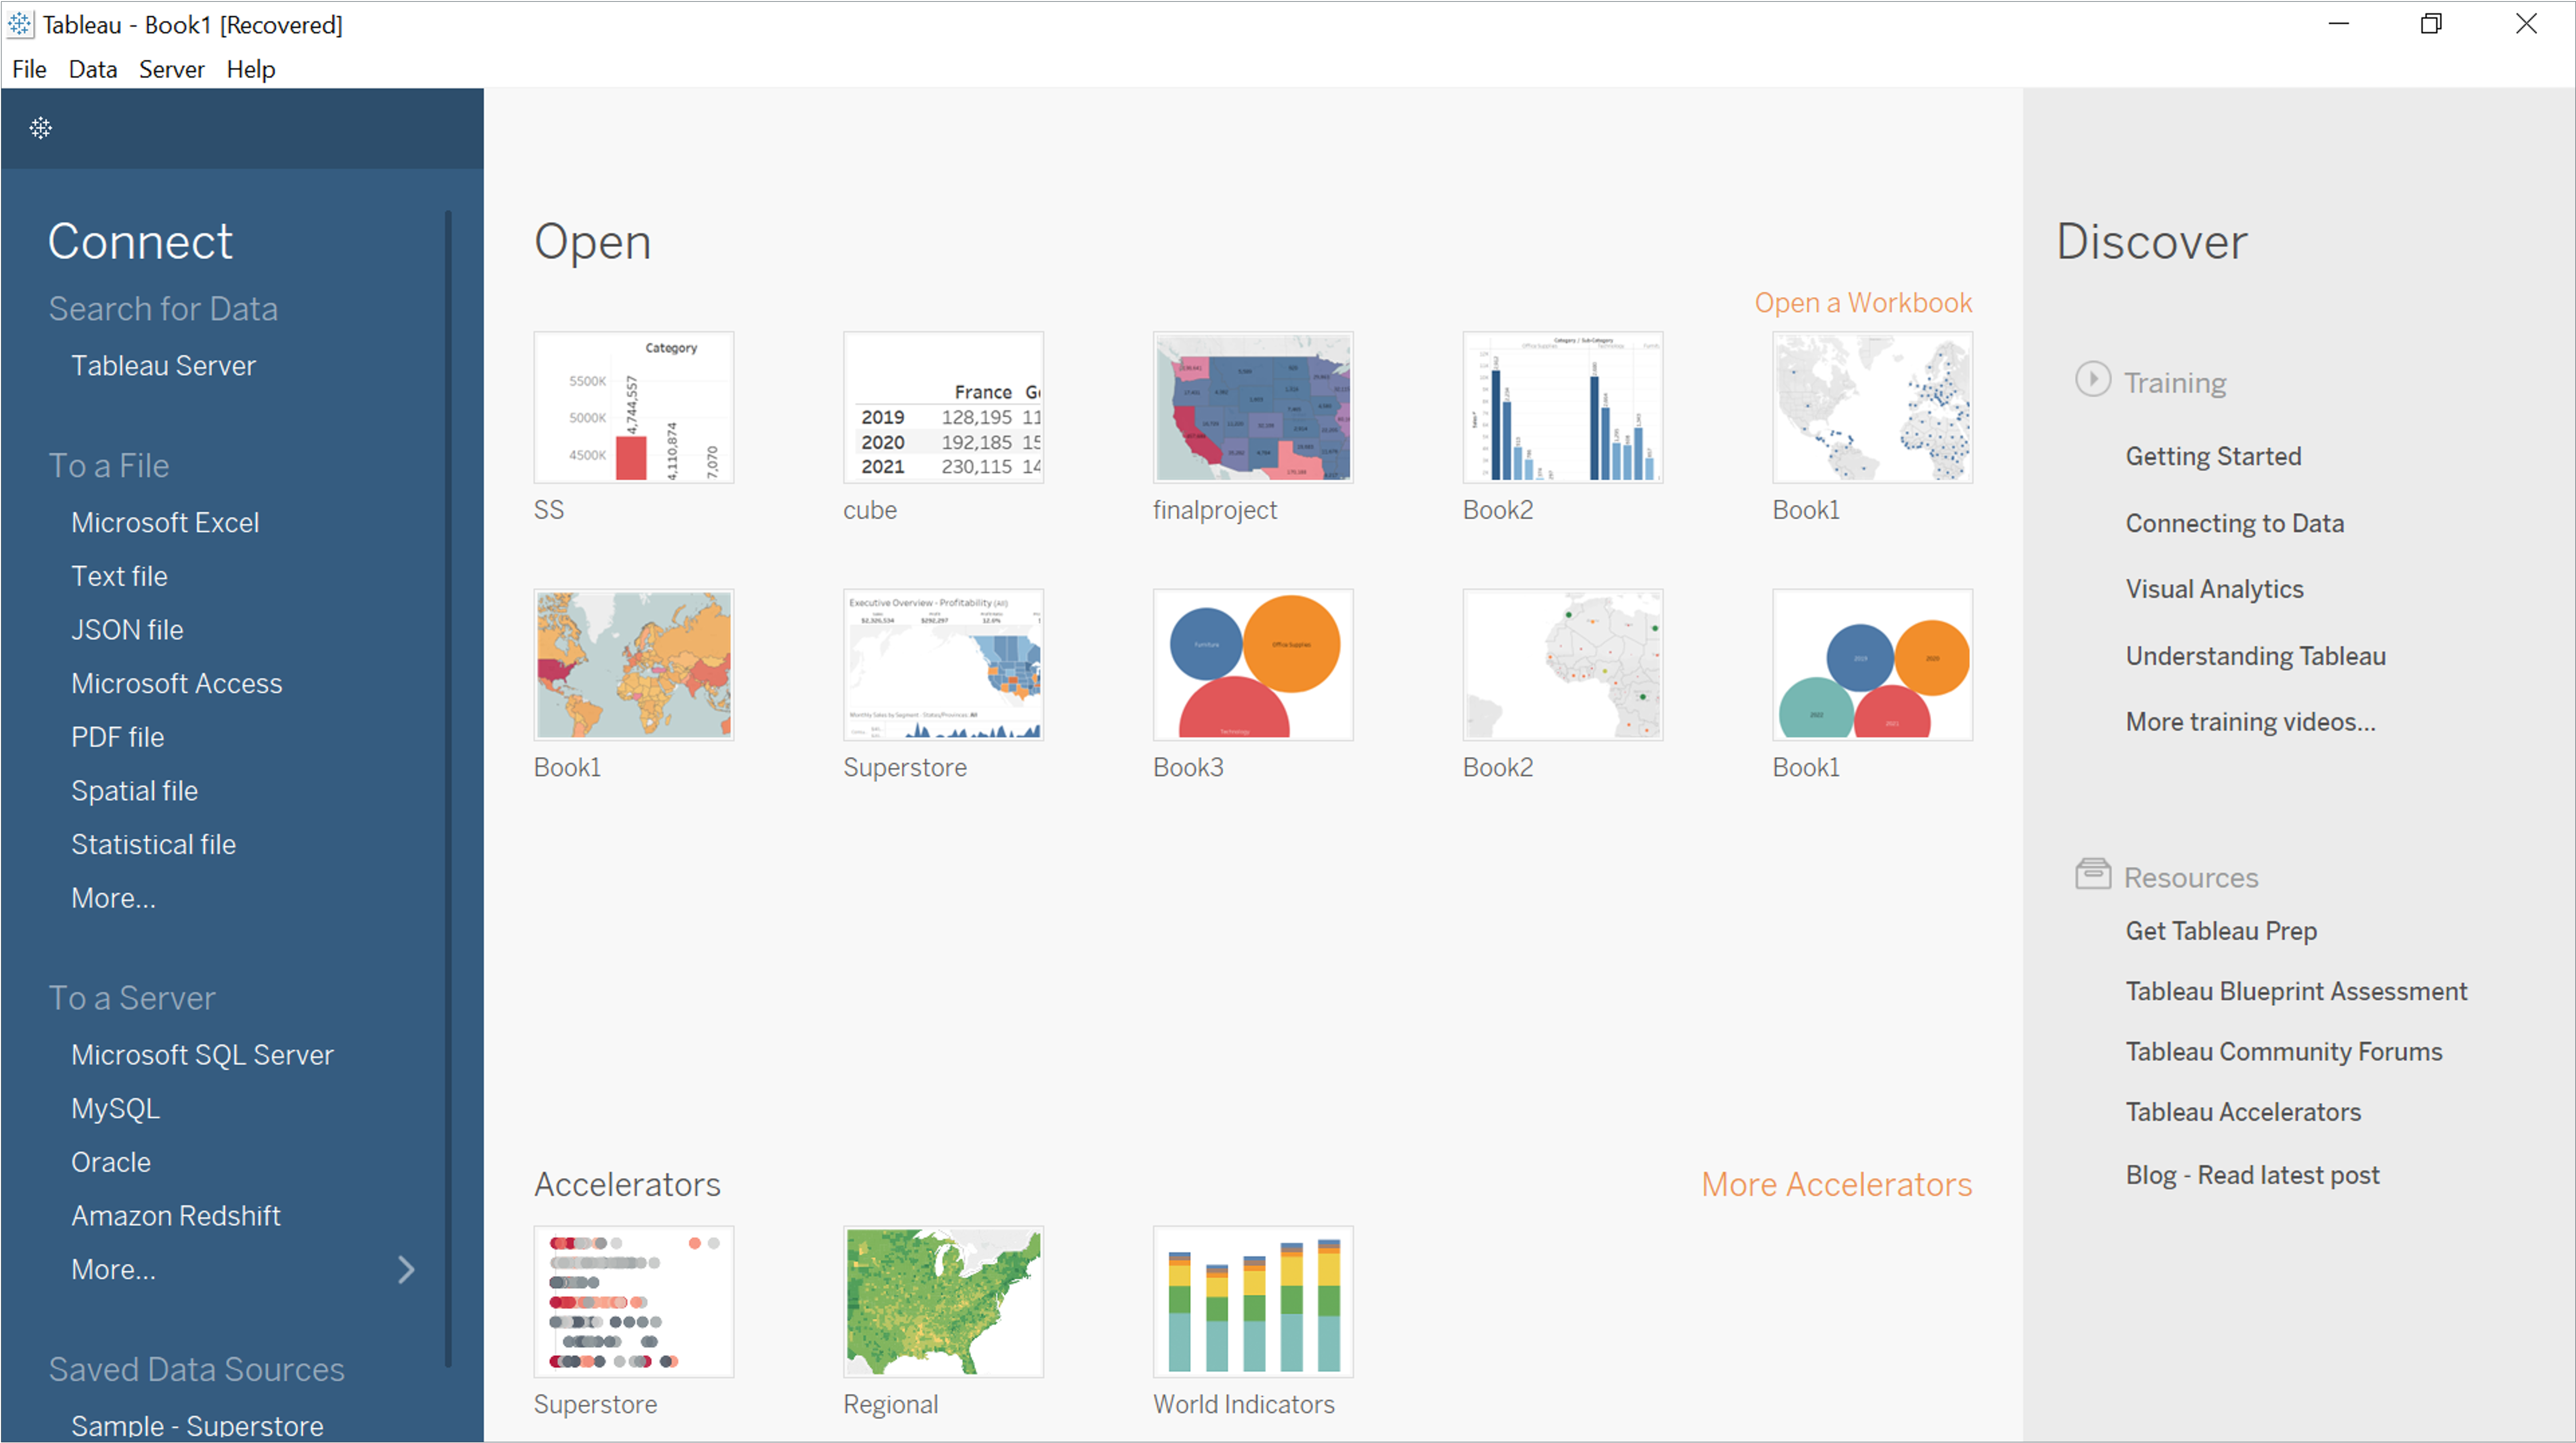
\includegraphics[width=0.8\textwidth]{./Picts/tab1.png}
    \caption{}
\end{figure}

Berikut ini adalah gambaran umum antarmuka pengguna Tableau seperti yang ditampilkan di atas:

\textbf{Open}: Buka buku kerja. Buku kerja Tableau adalah kumpulan berbagai jenis lembar kerja, seperti lembar kerja, dasbor, dan cerita.
\begin{figure}[H]
    \centering
    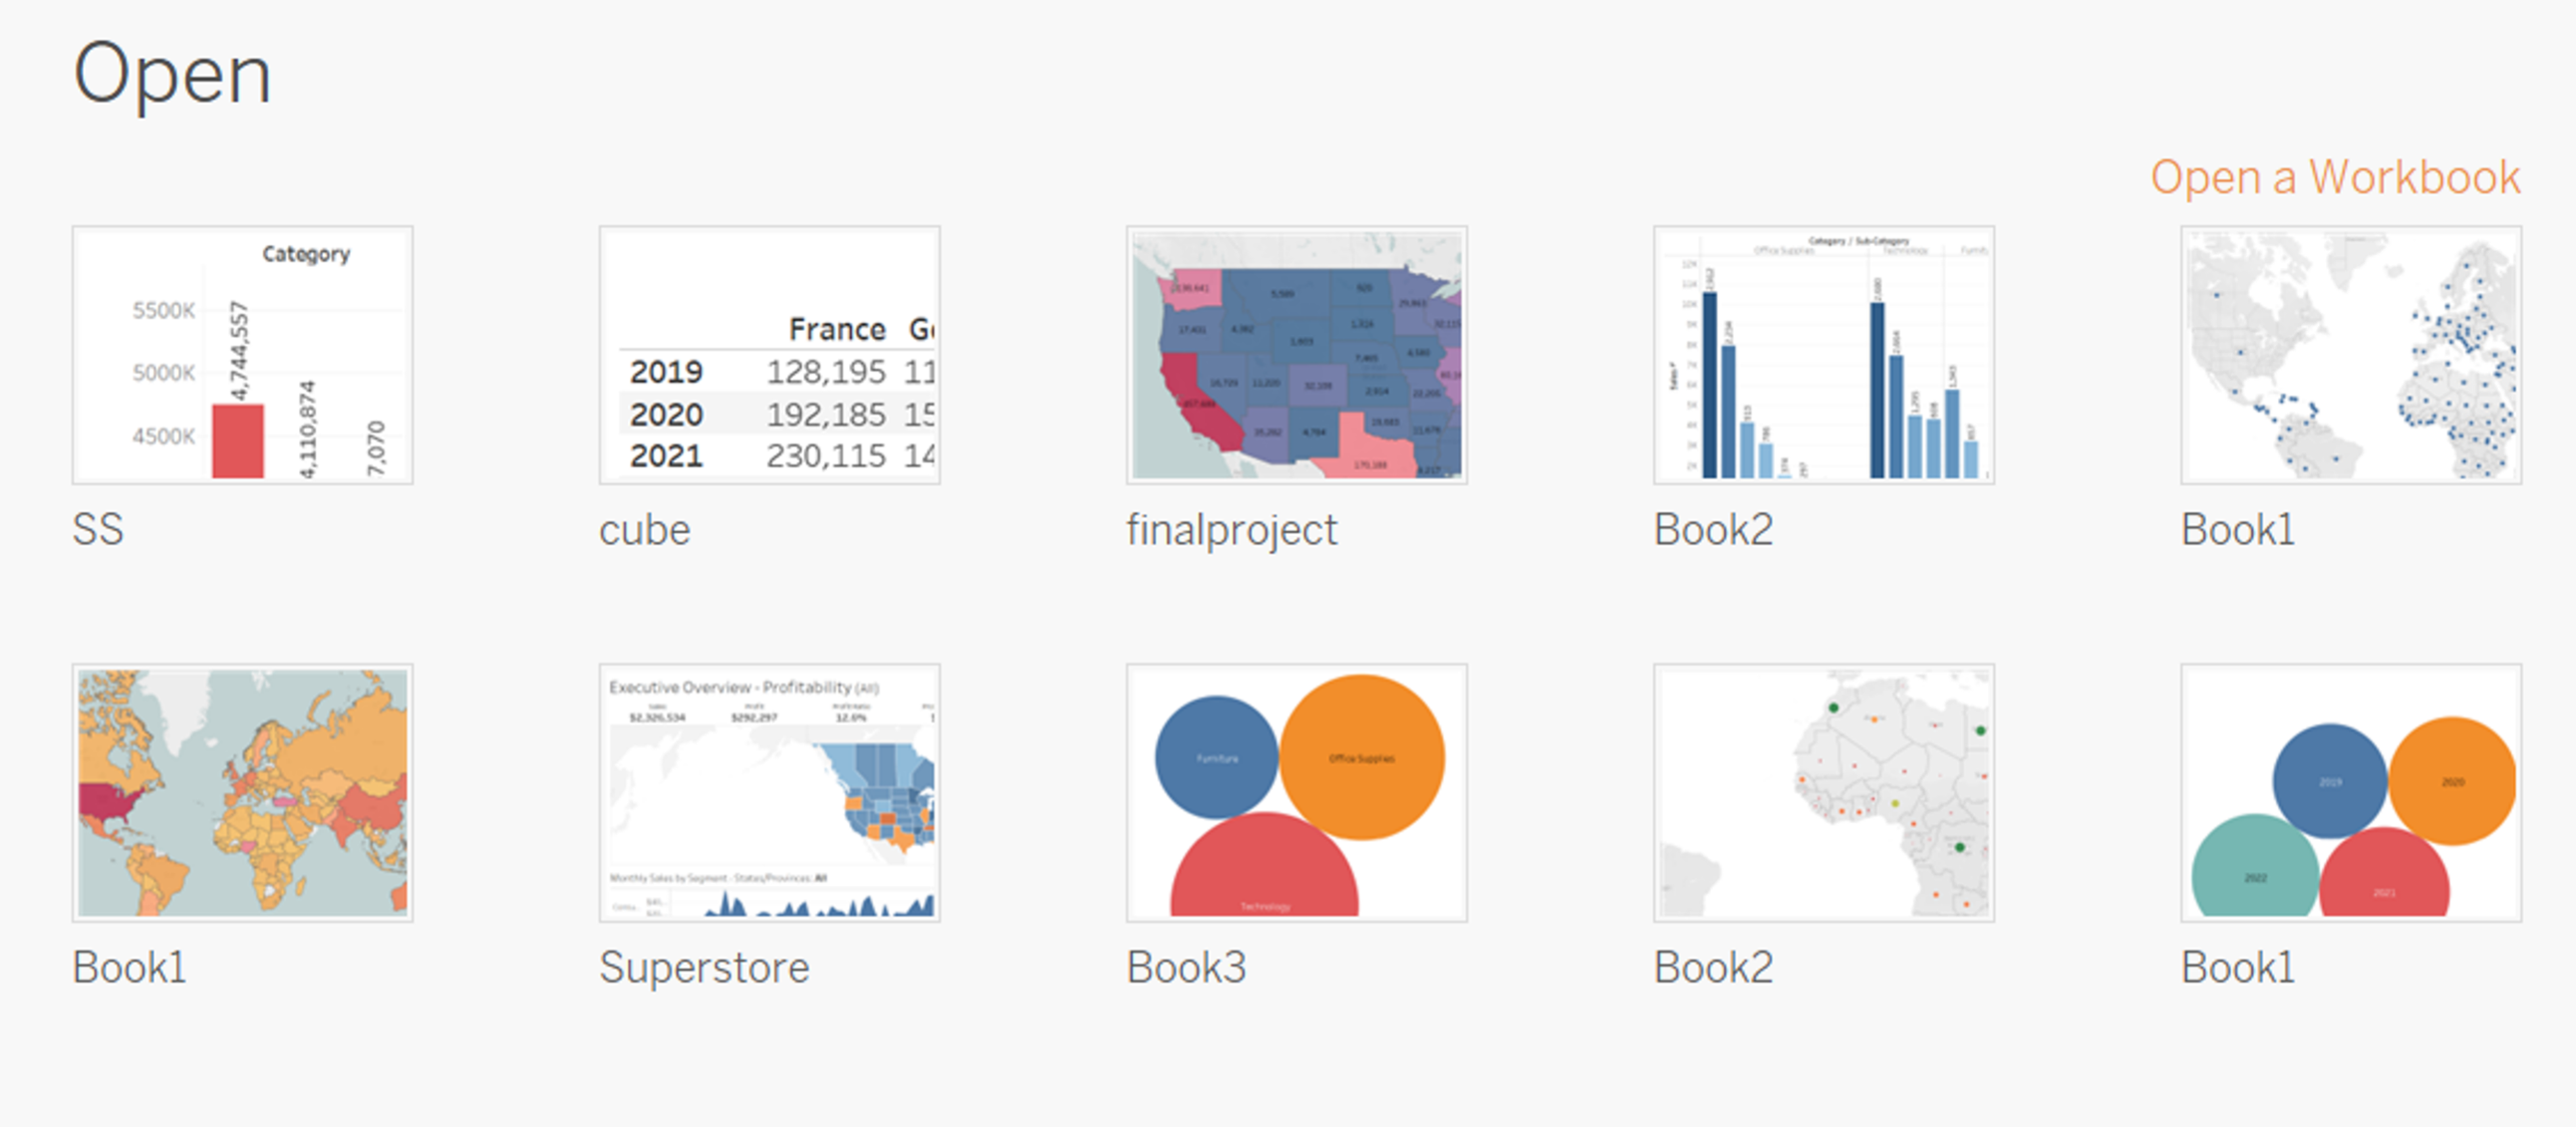
\includegraphics[width=0.8\textwidth]{./Picts/tab2.png}
    \caption{}
\end{figure}

\textbf{Accelerators}: Menyediakan buku kerja contoh.
\begin{figure}[H]
    \centering
    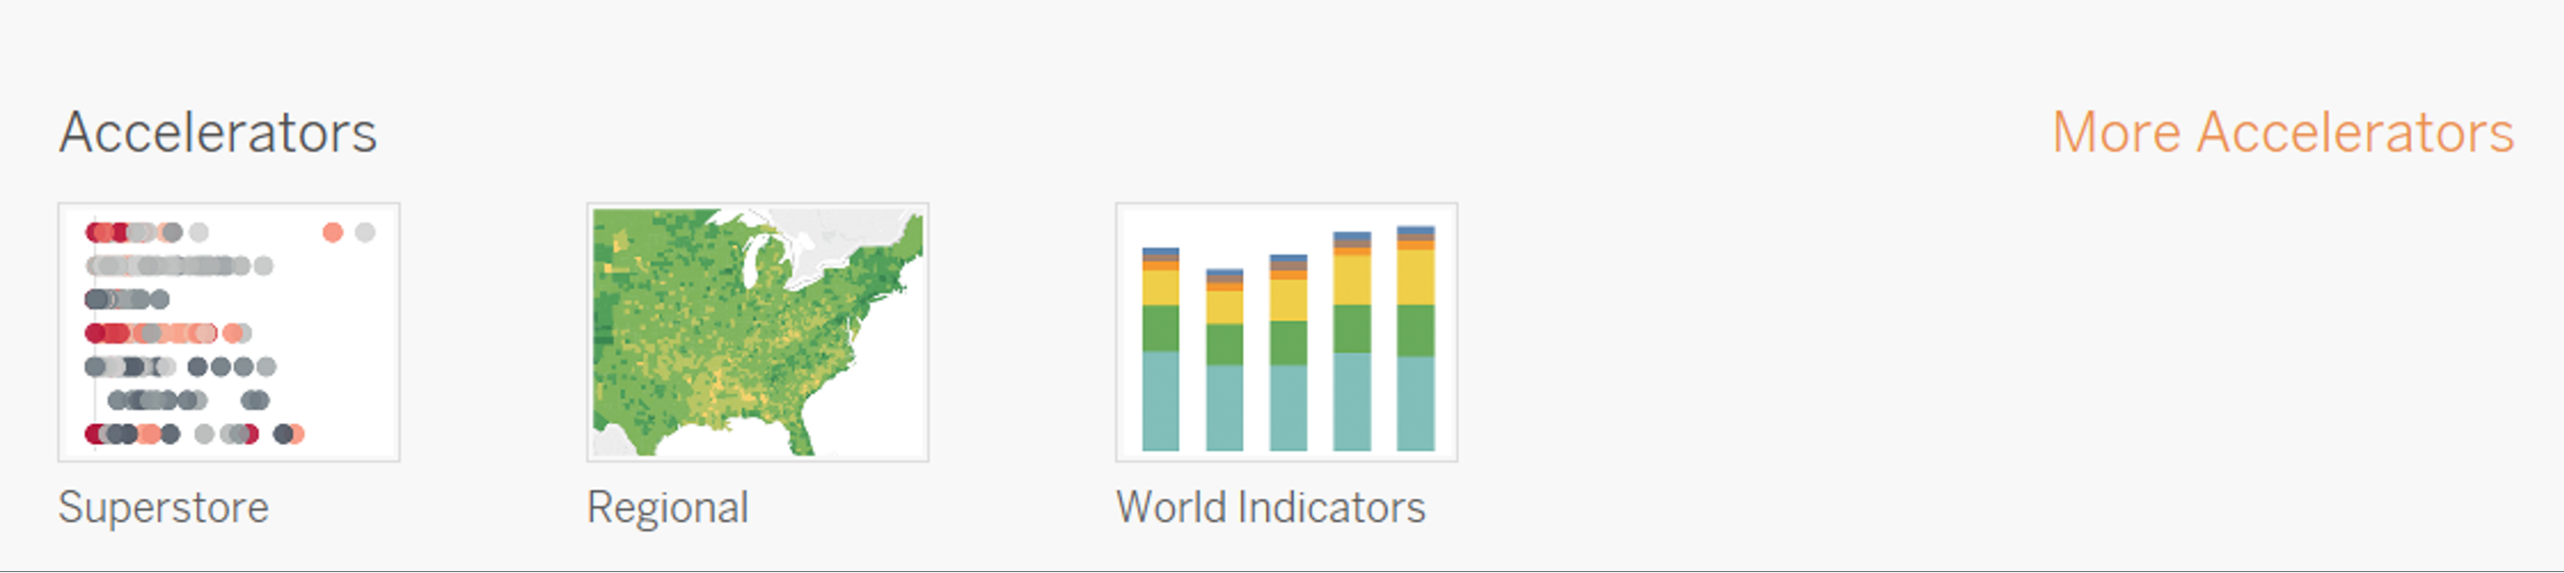
\includegraphics[width=0.8\textwidth]{./Picts/tab3.png}
    \caption{}
\end{figure}

\textbf{Discover}: Memberikan akses ke sumber belajar yang berguna seperti tutorial video, forum, dan blog.
\begin{figure}[H]
    \centering
    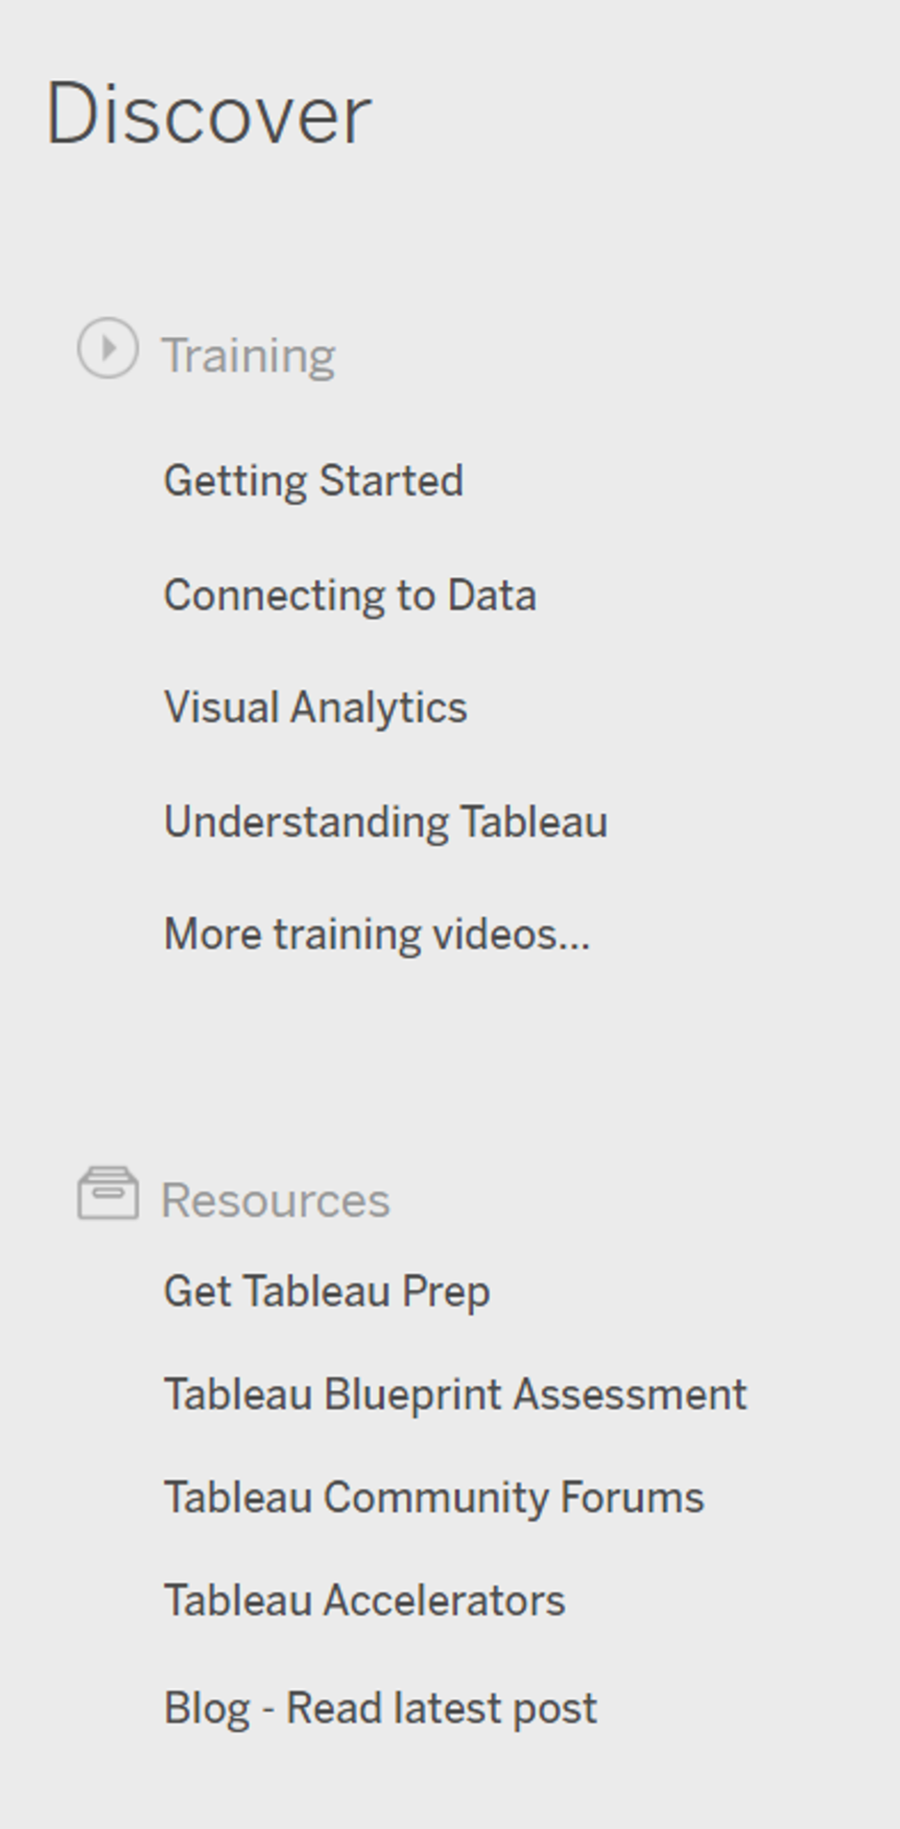
\includegraphics[width=0.8\textwidth]{./Picts/tab4.png}
    \caption{}
\end{figure}

\textbf{Logo Tableau}: Digunakan untuk beralih antara halaman awal dan ruang kerja penulisan.
\begin{figure}[H]
    \centering
    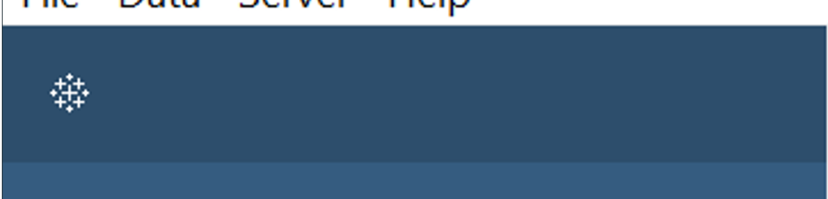
\includegraphics[width=0.8\textwidth]{./Picts/tab5.png}
    \caption{}
\end{figure}

\textbf{Panel Koneksi}: Digunakan untuk terhubung ke data dari berbagai sumber data. Ada beberapa jenis file dan server yang dapat Anda hubungkan melalui bagian Koneksi, seperti Microsoft Excel, file spasial, MySQL, dan banyak lagi.
\begin{figure}[H]
    \centering
    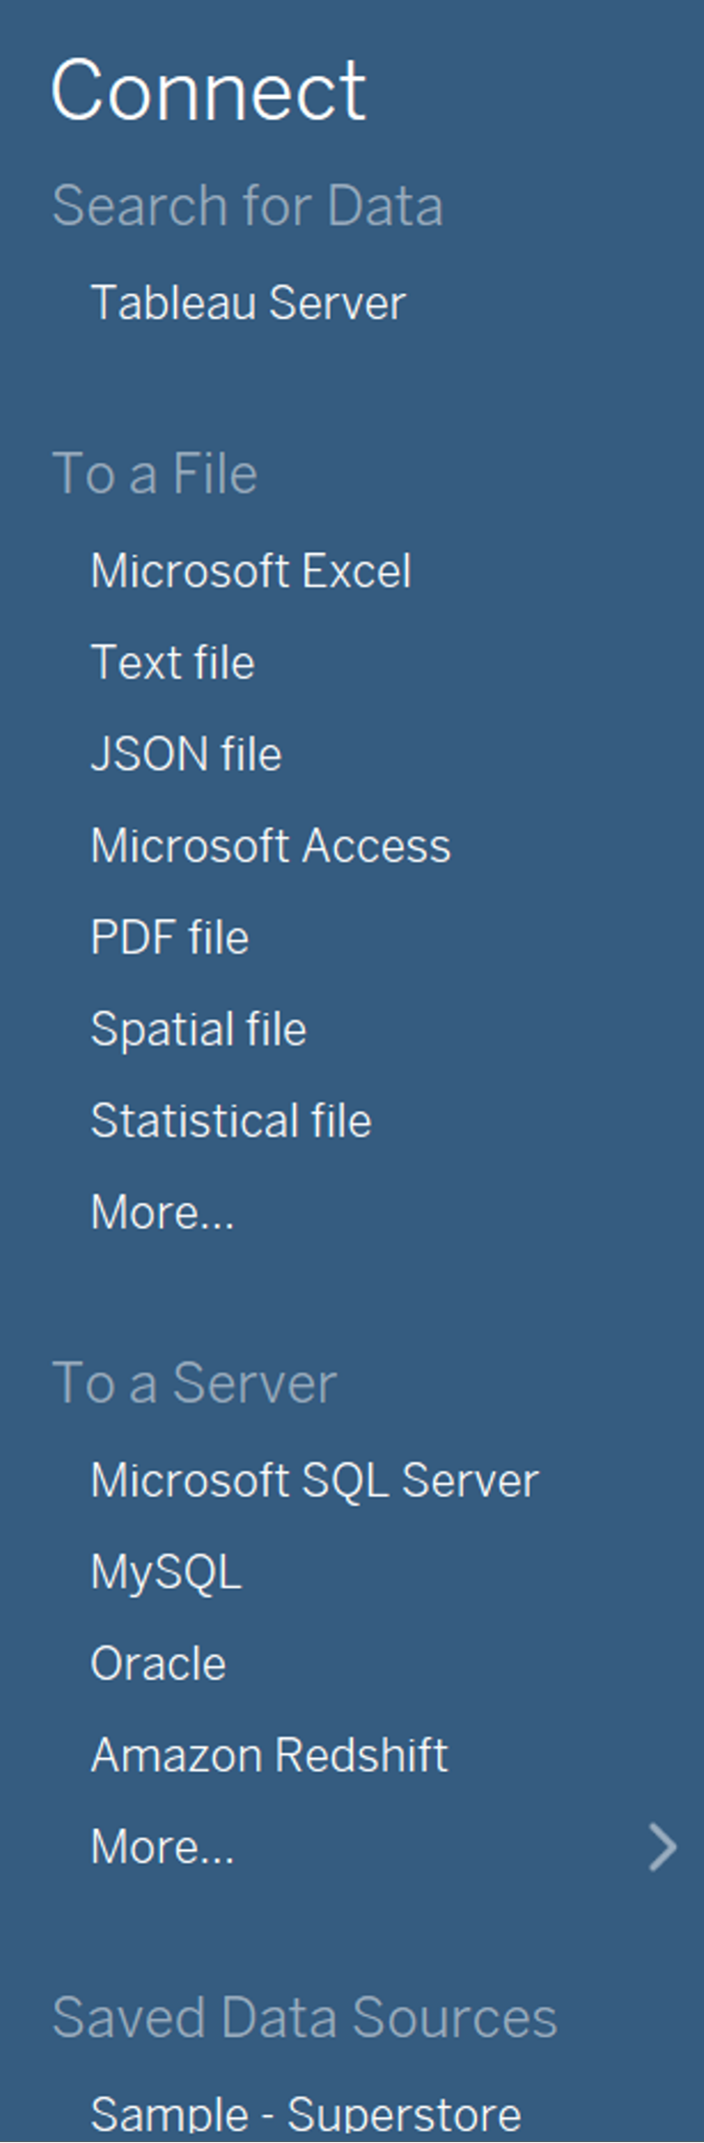
\includegraphics[width=0.8\textwidth]{./Picts/tab6.png}
    \caption{}
\end{figure}

\subsubsection{Memvisualkan Data}
Seperti yang Anda ketahui, Tableau digunakan untuk memvisualisasikan data. Ada banyak cara untuk memvisualisasikan data Anda di Tableau, termasuk:
\begin{itemize}
    \item Grafik batang.
    \item Grafik tren.
    \item Dan grafik peta.
\end{itemize}

Mari kita tinjau langkah-langkah untuk membuat jenis grafik yang berbeda ini.


\subsubsection{Membuat Diagram Batang}
Untuk memulai analisis data Global Super Store, pilih Microsoft Excel. Navigasi ke sumber data di komputer Anda dan pilih file Global Super Store.

Tindakan ini akan memuat data file ke dalam panel Data Tableau, yang berisi informasi tentang semua pesanan yang dibuat di Global Super Store, termasuk produk, penjualan, pelanggan, dan data pengiriman.
\begin{figure}[H]
    \centering
    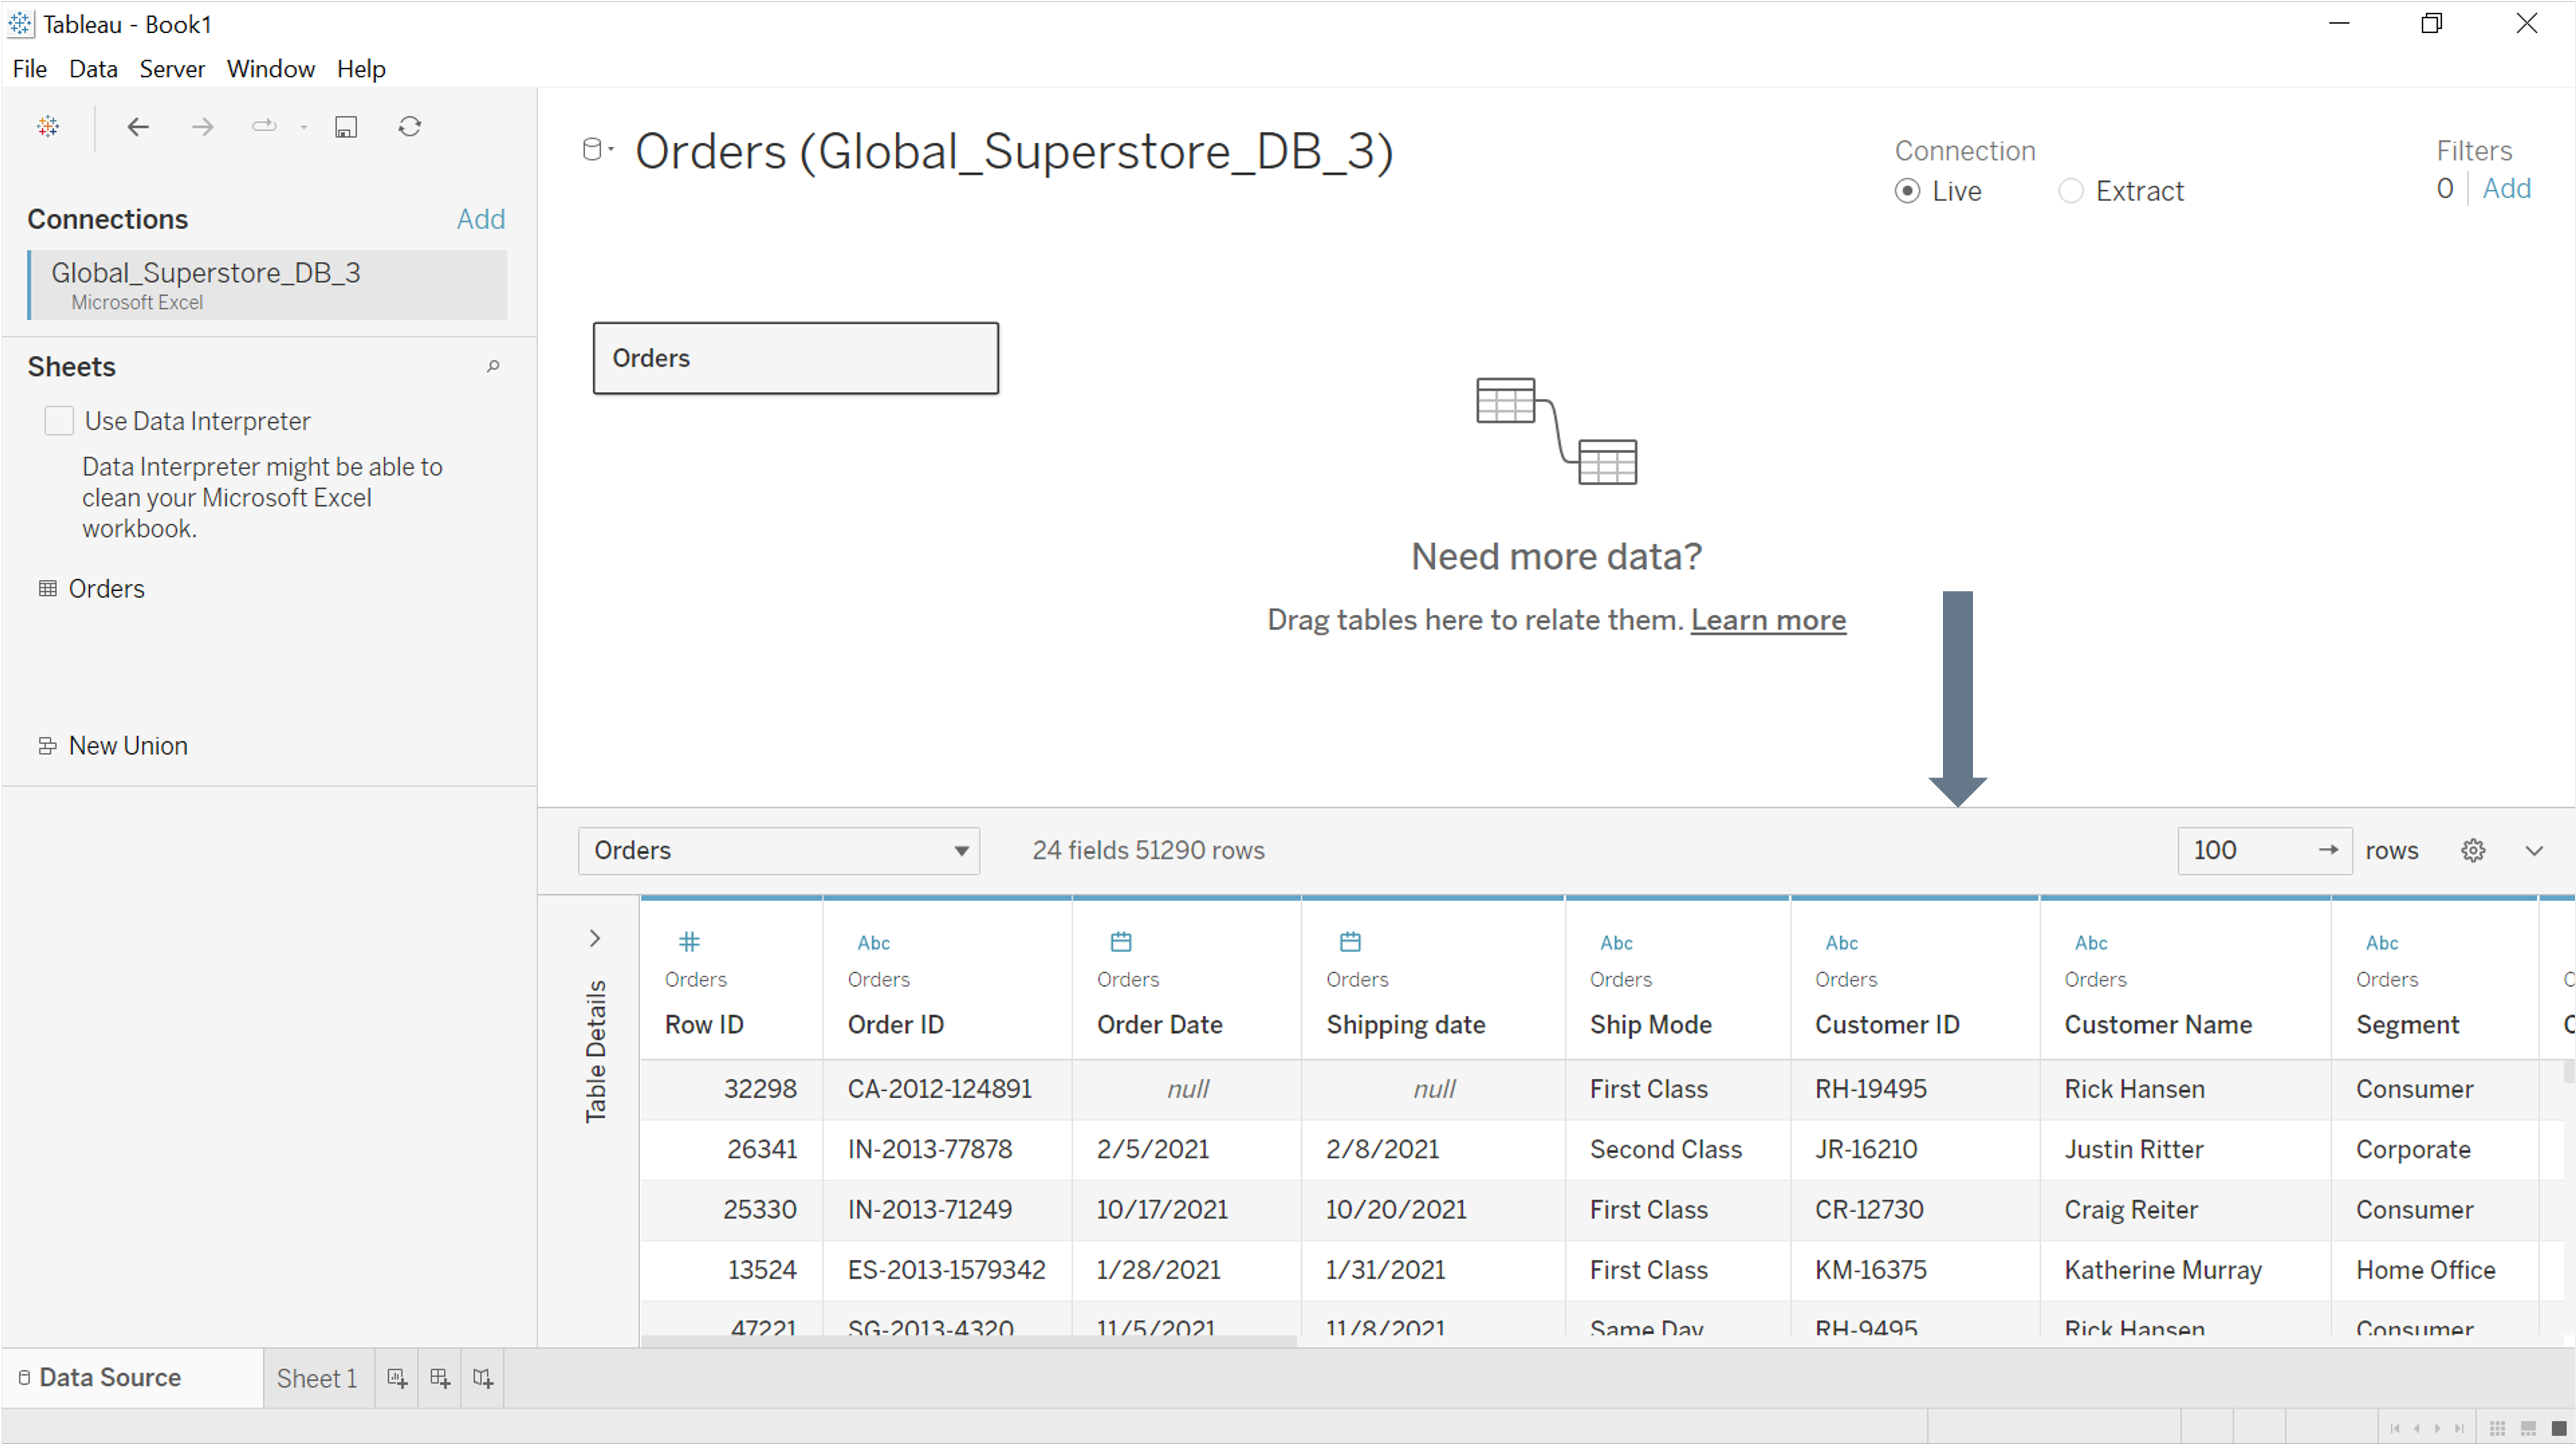
\includegraphics[width=0.8\textwidth]{./Picts/tab7.png}
    \caption{}
\end{figure}

Sekarang Anda perlu membuat diagram batang yang menampilkan total penjualan di semua kategori produk. Anda dapat menganalisis hasil tersebut dan menentukan cara untuk meningkatkan penjualan. Pilih tab lembar kerja untuk memulai analisis data dan membuat visualisasi data Global Super Store.

\begin{figure}[H]
    \centering
    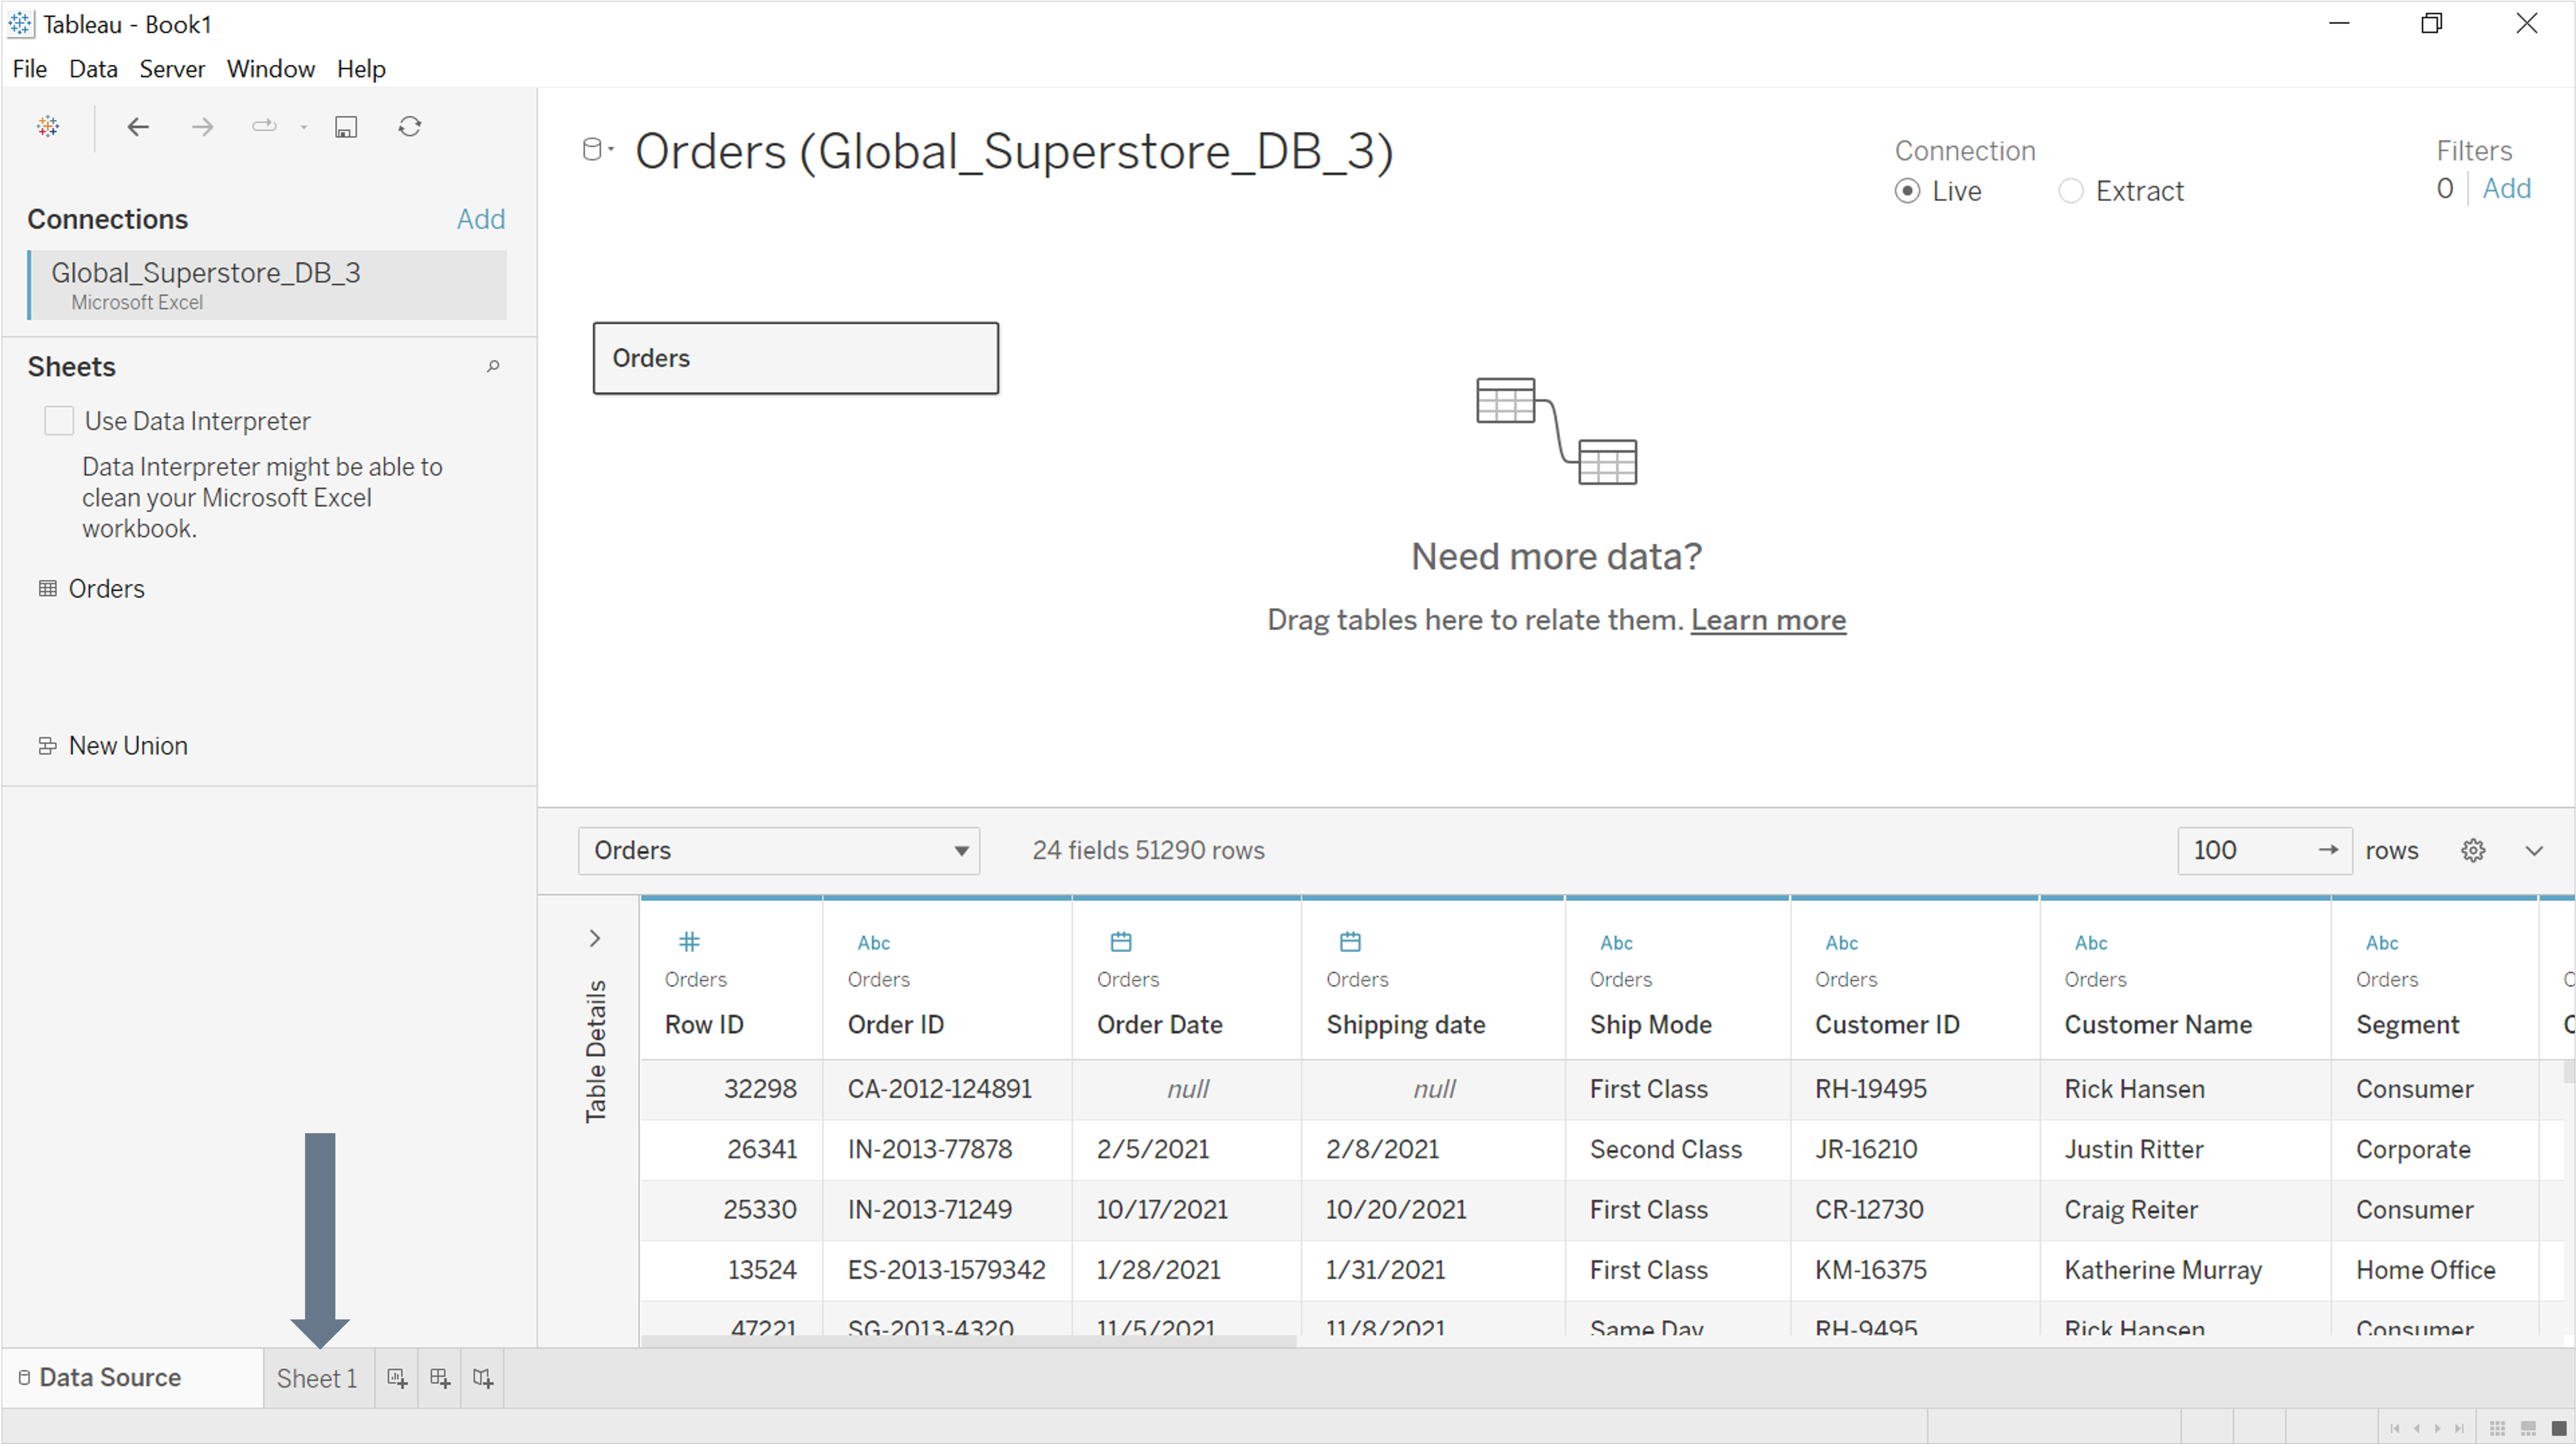
\includegraphics[width=0.8\textwidth]{./Picts/tab8.png}
    \caption{}
\end{figure}

Tindakan ini akan mengalihkan Anda ke ruang pengeditan lembar kerja.

\begin{figure}[H]
    \centering
    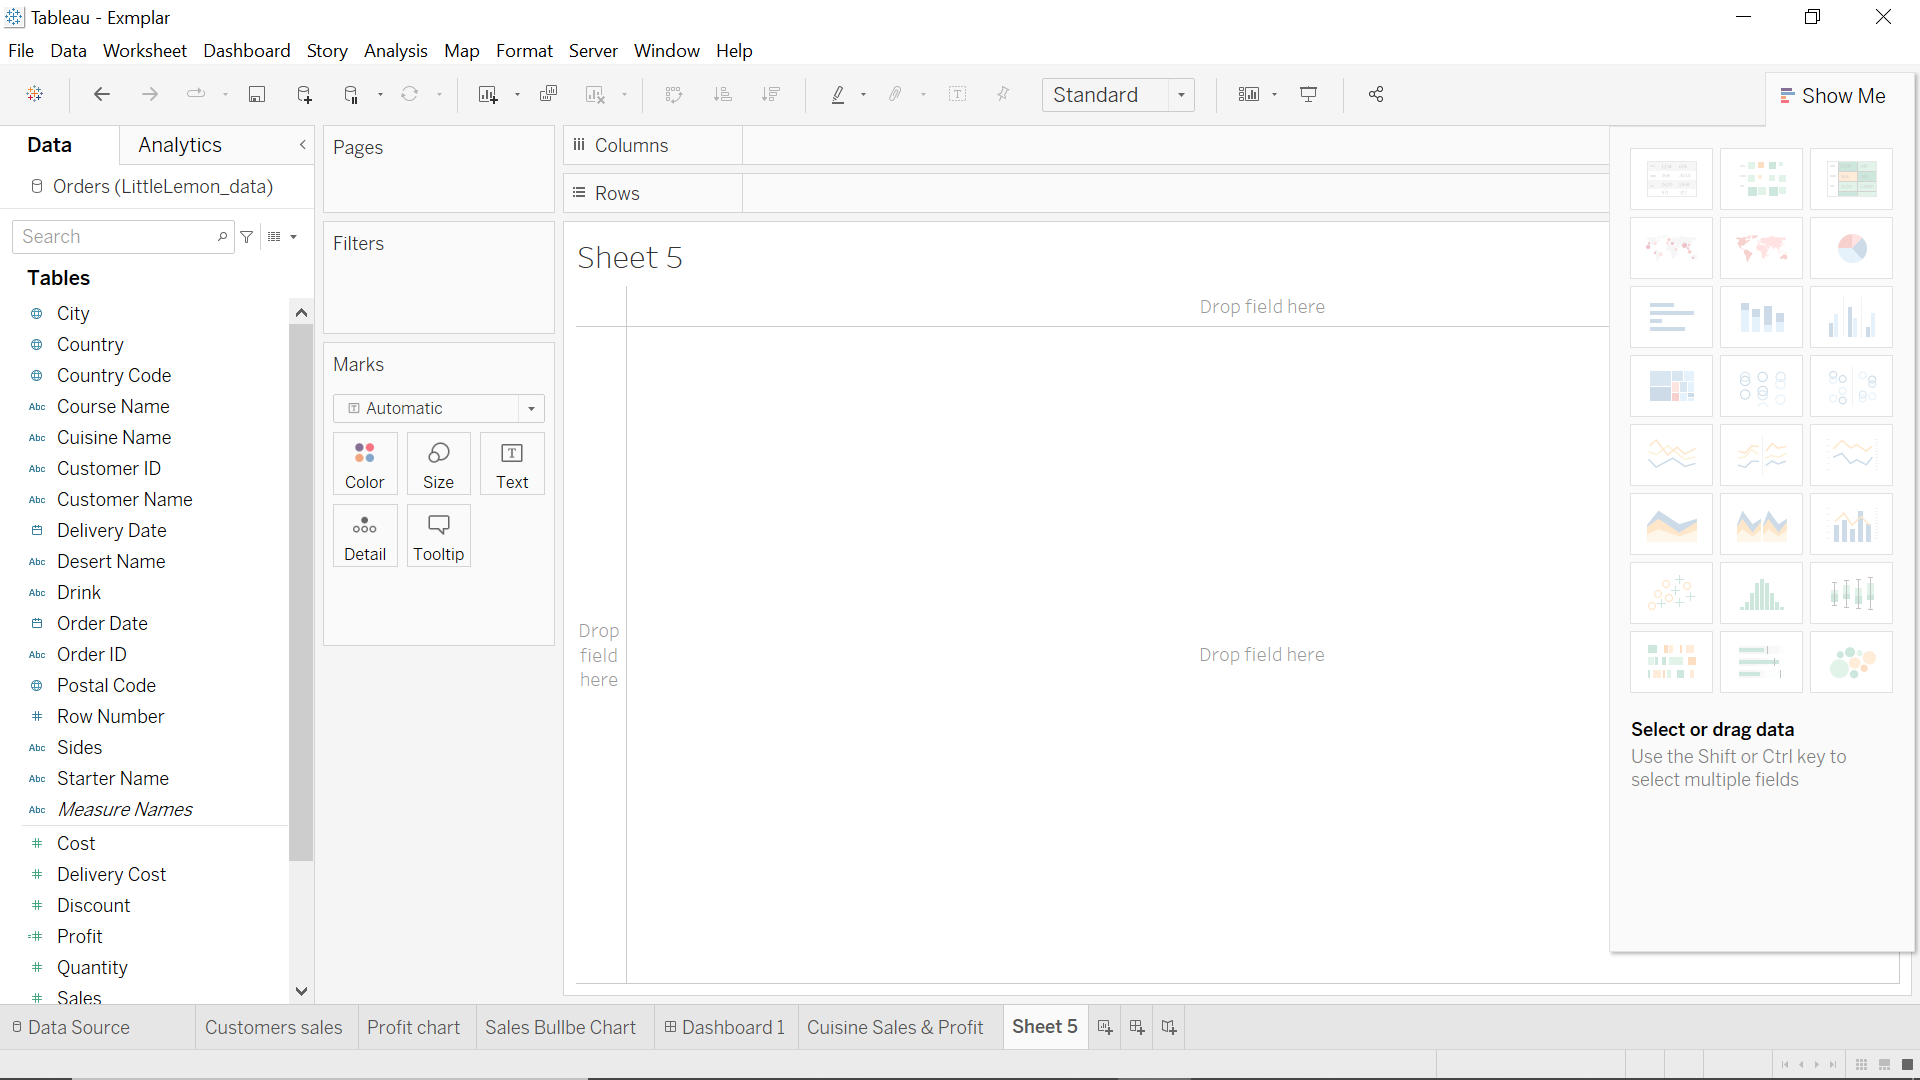
\includegraphics[width=0.8\textwidth]{./Picts/tab9.png}
    \caption{}
\end{figure}

Di dalam ruang authoring ini, Anda dapat menyeret dan meletakkan bidang dimensi dan ukuran yang relevan langsung ke area kanvas.

\begin{figure}[H]
    \centering
    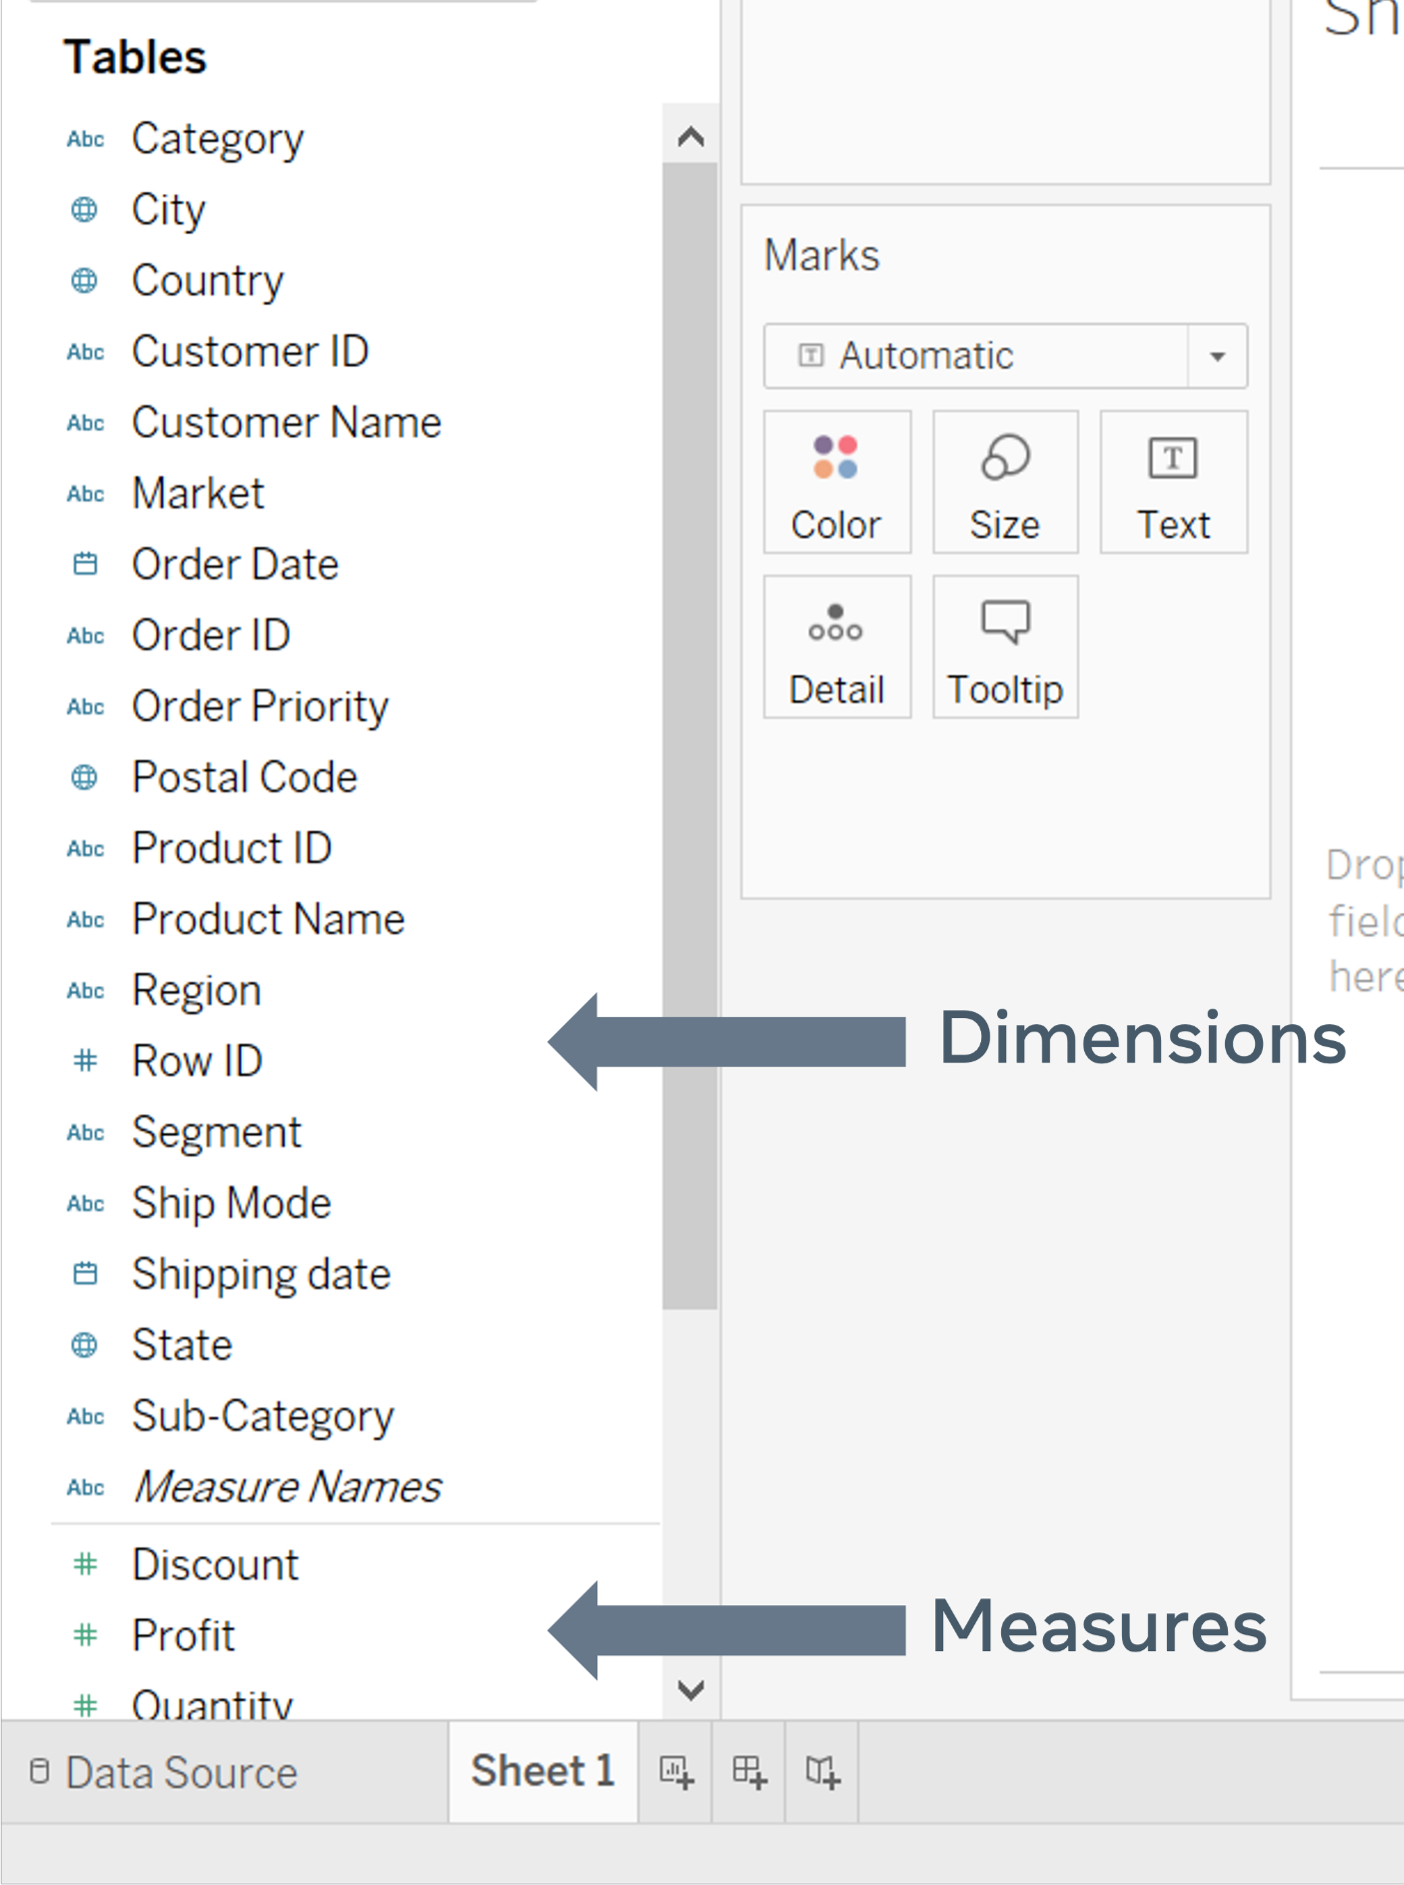
\includegraphics[width=0.8\textwidth]{./Picts/tab10.png}
    \caption{}
\end{figure}

Anda dapat memindahkan data ke area kartu, atau ke kolom dan baris di bagian rak.

\begin{figure}[H]
    \centering
    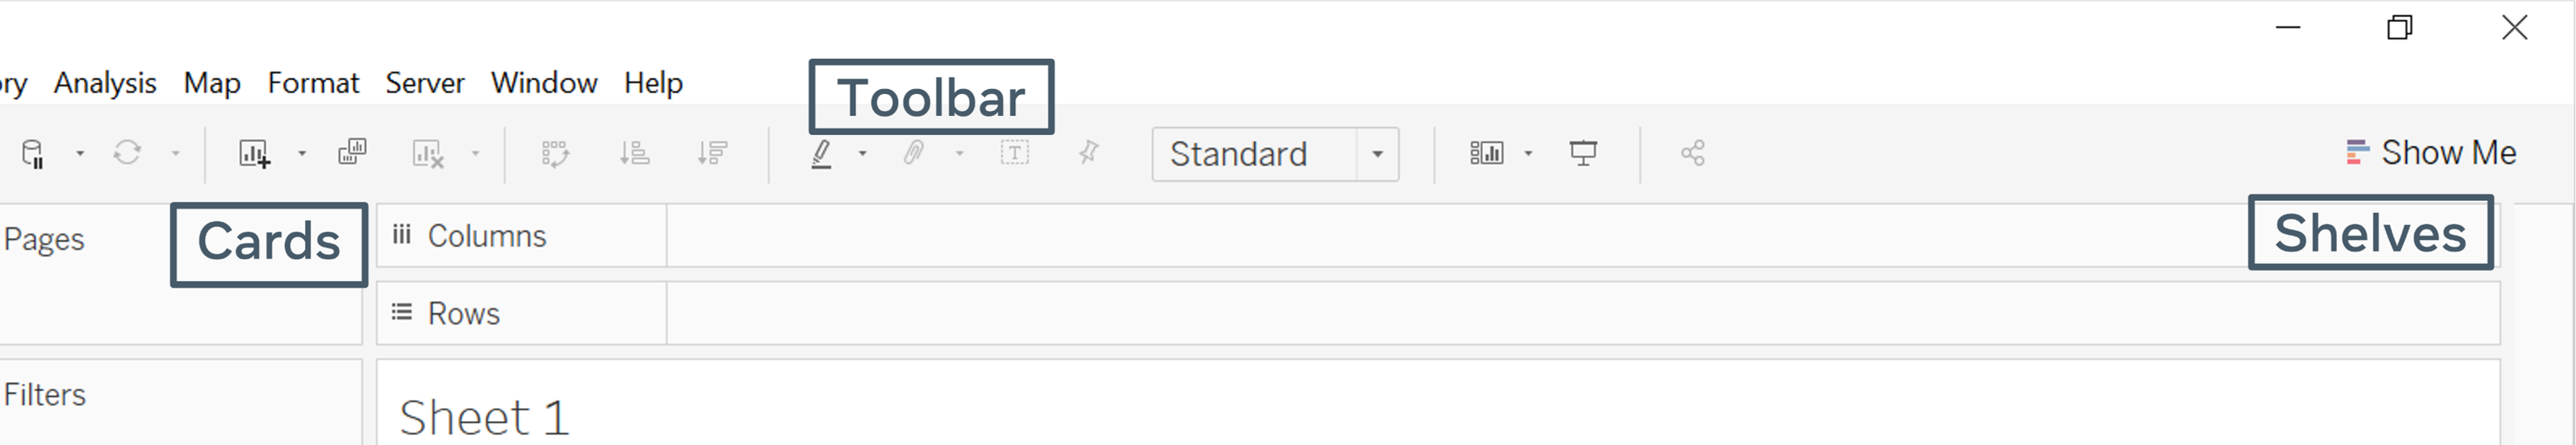
\includegraphics[width=0.8\textwidth]{./Picts/tab11.png}
    \caption{}
\end{figure}

Untuk menyelesaikan tugas Anda, seret opsi kategori ke rak kolom dan opsi penjualan ke rak baris. Hal ini akan menghasilkan diagram batang dengan informasi yang relevan.

\begin{figure}[H]
    \centering
    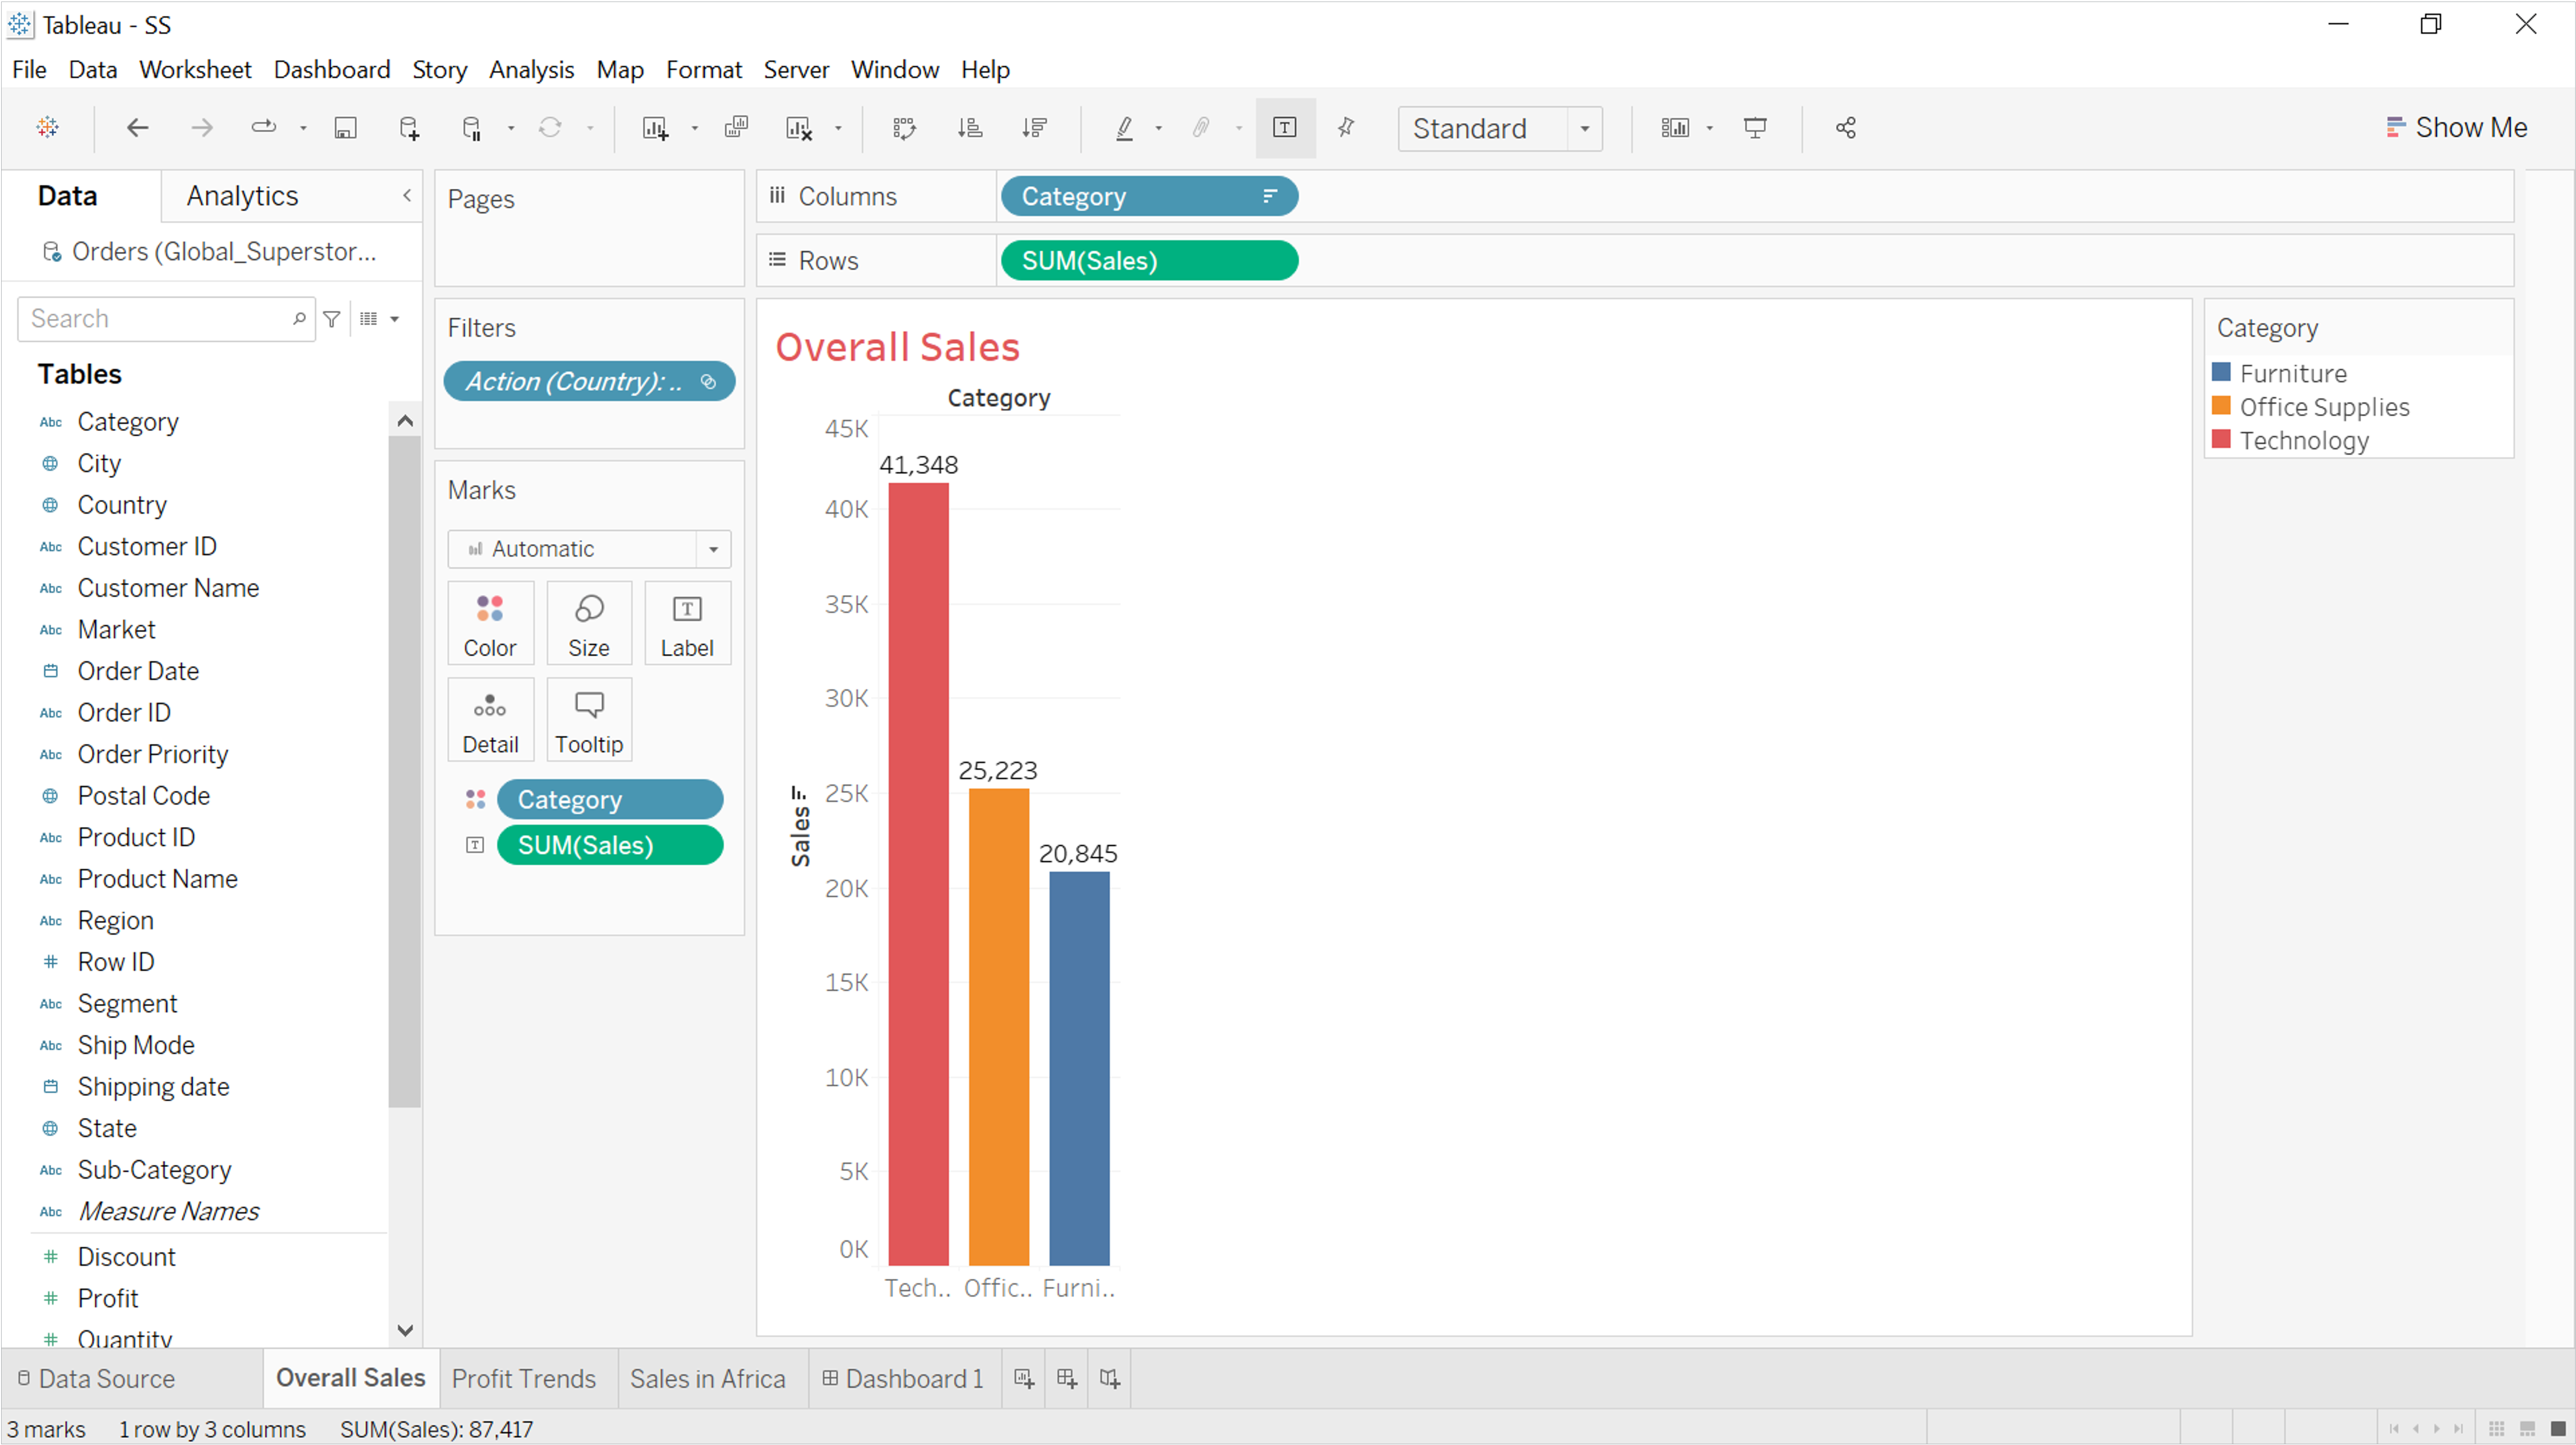
\includegraphics[width=0.8\textwidth]{./Picts/tab12.png}
    \caption{}
\end{figure}

Anda juga dapat melakukan beberapa perubahan pada tampilan grafik untuk membuatnya lebih menarik secara visual:
\begin{itemize}
    \item Atur batang grafik dalam urutan naik atau turun menggunakan ikon terkait di bilah alat.
    \item Seret bidang kategori dari panel Data ke kotak Warna pada kartu Marks.
    \item Seret bidang penjualan dari panel Data ke kotak Label pada kartu Marks.
    \item Berikan lembar kerja dengan nama yang bermakna.
\end{itemize}

\subsubsection{Membuat Diagram Trend}
Anda telah membuat diagram batang yang menampilkan penjualan untuk semua kategori. Selanjutnya, Anda perlu membuat tampilan baru di mana Anda dapat menganalisis tren keuntungan per kategori selama beberapa tahun terakhir. Diagram tren paling cocok untuk tugas ini. Ikuti langkah-langkah berikut untuk menyelesaikan tugas ini:
\begin{itemize}
    \item Seret bidang Tanggal Pesanan dari panel Data ke rak kolom.
    \item Seret bidang Laba dari panel Data ke rak baris.
    \item Seret bidang kategori dari panel Data ke kotak Warna pada kartu Tanda.
    \item Seret bidang kategori dari panel Data ke kotak Label pada kartu Tanda.
    \item Berikan lembar kerja dengan nama yang bermakna.
\end{itemize}

\begin{figure}[H]
    \centering
    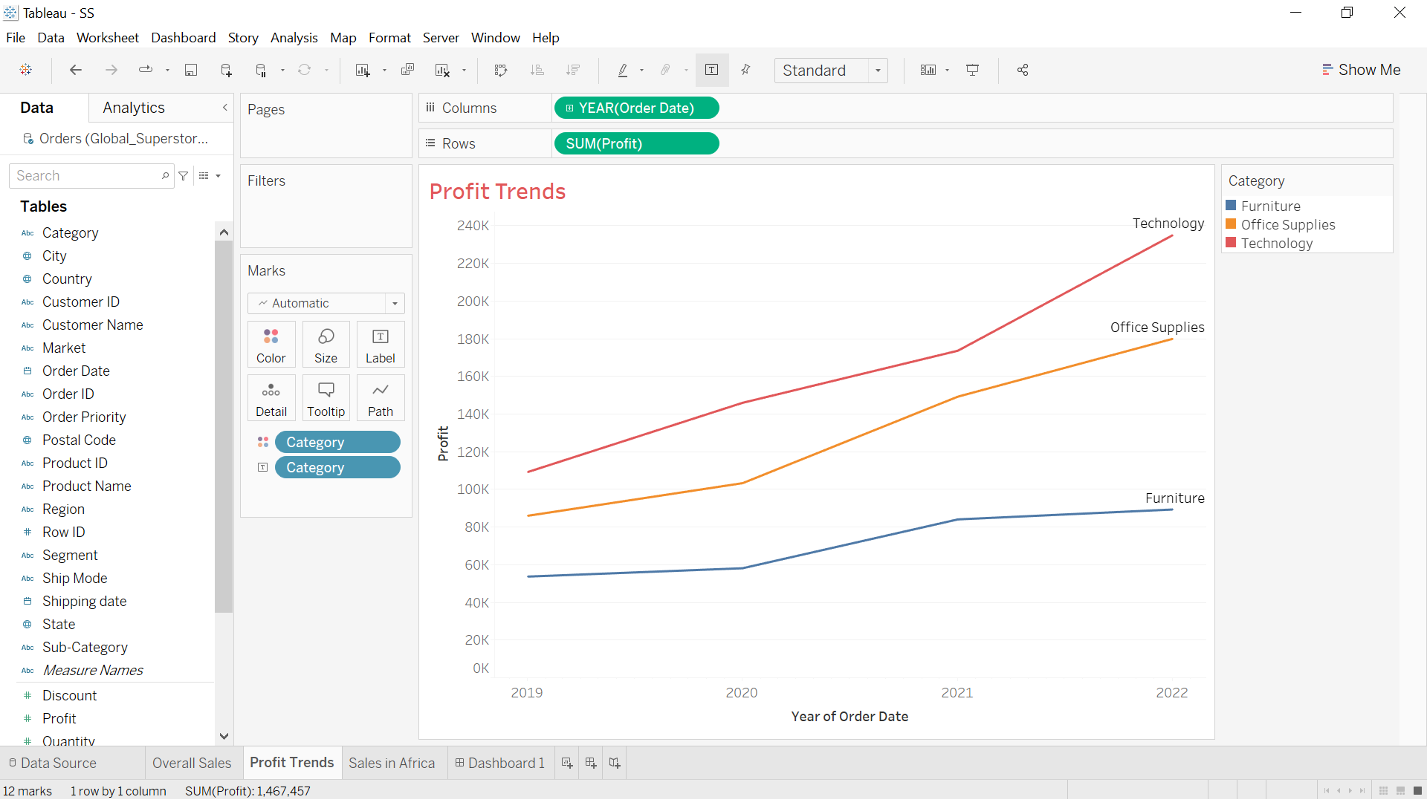
\includegraphics[width=0.8\textwidth]{./Picts/tab13.png}
    \caption{}
\end{figure}

\subsubsection{Membuat Diagram Peta}
Tugas Anda selanjutnya adalah menganalisis penjualan dan laba Global Super Store di Afrika, serta menentukan negara mana yang menjadi pasar terbaik bagi perusahaan. Anda dapat menggunakan peta untuk menyelesaikan tugas ini. Ikuti langkah-langkah berikut untuk menyelesaikan tugas ini:
\begin{itemize}
    \item Klik ganda bidang Negara di panel Data untuk membuat peta di area kanvas.
    \item Seret bidang Wilayah dari panel Data ke kartu Filter Baris, lalu pilih Afrika.
    \item Seret bidang Negara dari panel Data ke kotak Warna di kartu Tanda.
    \item Seret bidang Penjualan dari panel Data ke kotak Ukuran di kartu Tanda.
    \item Seret bidang Laba dari panel Data ke kotak Tooltip di kartu Tanda.
    \item Berikan lembar kerja dengan nama yang bermakna.
\end{itemize}

Anda sekarang memiliki beberapa jenis grafik yang berbeda yang dapat digunakan untuk mengidentifikasi tren dan pola penjualan. Global Super Store dapat menggunakan grafik-grafik ini untuk membandingkan data penjualan mereka dan mengambil keputusan bisnis.

\begin{figure}[H]
    \centering
    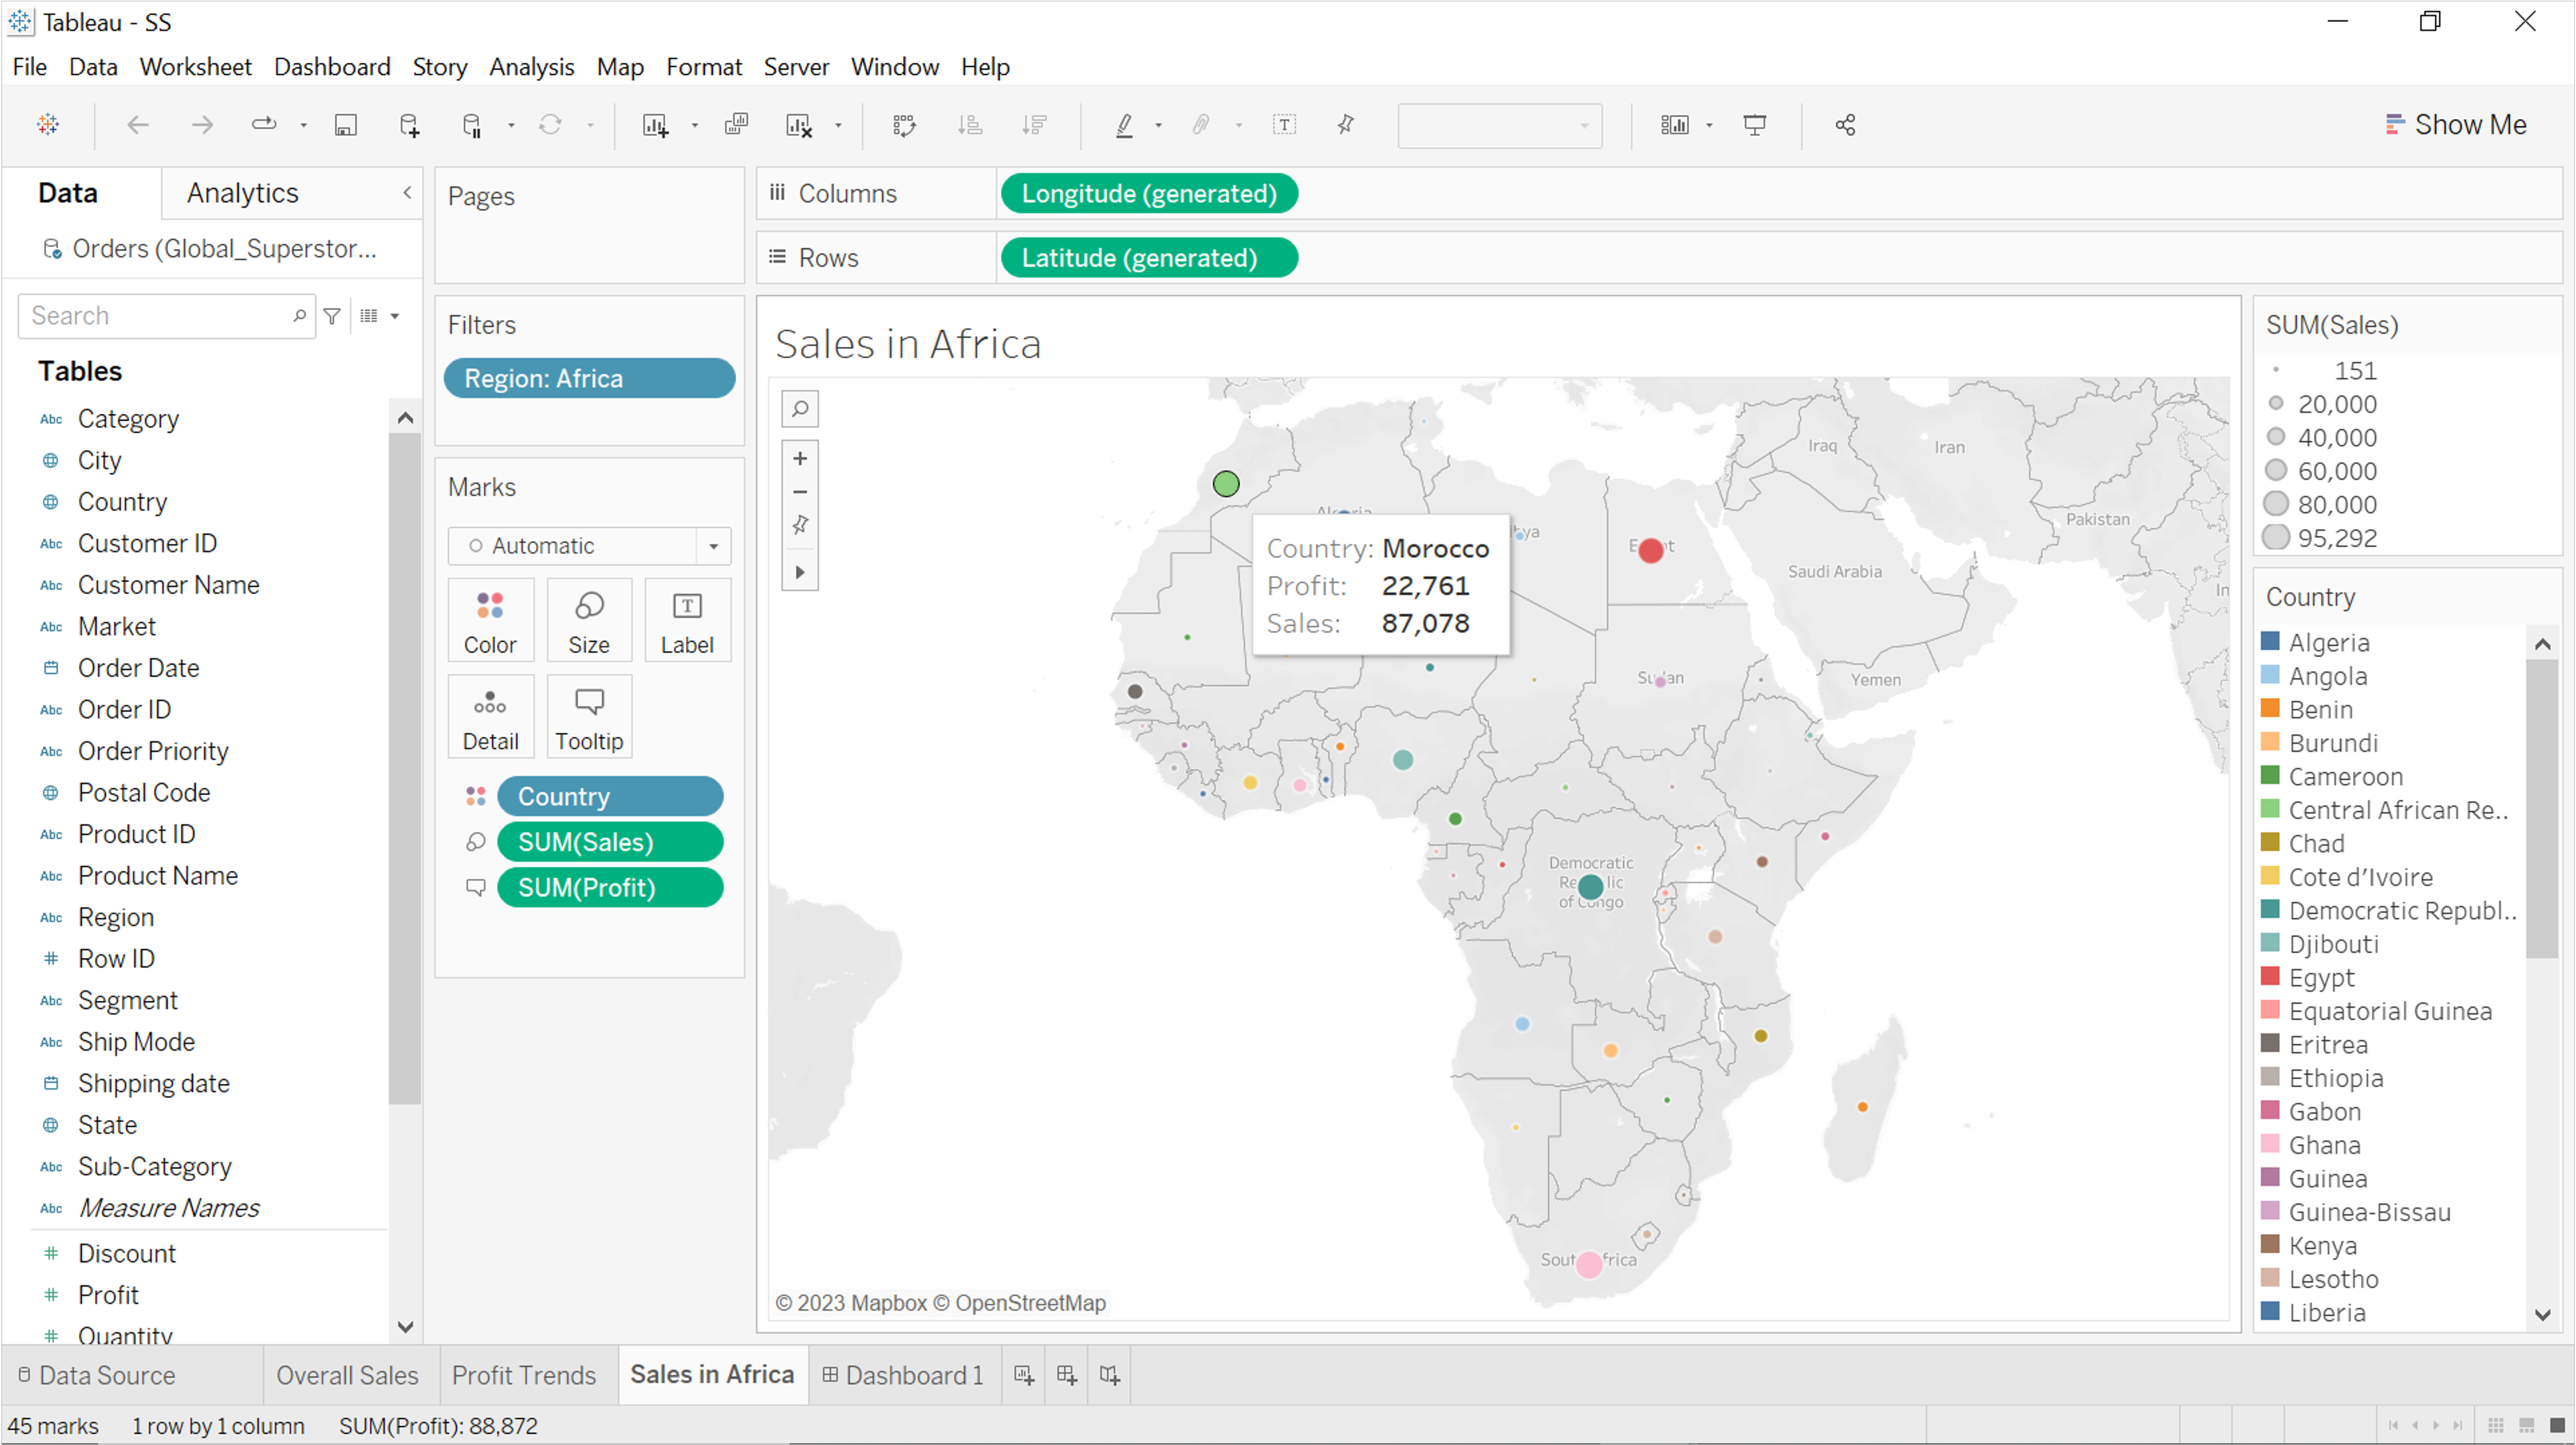
\includegraphics[width=0.8\textwidth]{./Picts/tab14.png}
    \caption{}
\end{figure}

\subsection{Data Import dan Data Preparation di Tableau}
\subsubsection{Menghubungkan Tableau ke Sumber Data}
Buka Tableau dan pilih "Microsoft Excel" di tab Connect untuk menghubungkan ke file Excel.

Live Connection: Dengan koneksi langsung, pembaruan pada sumber asli akan otomatis tercermin di database Tableau.

\subsubsection{Membersihkan dan Menyiapkan Data}
\begin{itemize}
    \item Metadata Grid: Menampilkan informasi tentang berbagai field data. Anda dapat menyembunyikan atau menampilkan grid ini sesuai kebutuhan.
    \item Operasi Pembersihan: Meliputi filtering, sorting, dan renaming data untuk memudahkan analisis.
\end{itemize}

\subsubsection{Mengubah Tipe Data dan Mengelola Kolom}
\begin{itemize}
    \item Mengubah Tipe Data: Klik panah kecil di atas kolom (misalnya, Order Date) dan pilih "Describe" untuk melihat informasi. Ubah tipe data menjadi "Date" jika diperlukan.
    \item Menyembunyikan Kolom: Pilih panah kecil dan pilih "Hide" untuk menyembunyikan kolom yang tidak relevan. Gunakan "Show Hidden Fields" untuk menampilkan kembali kolom yang disembunyikan.
\end{itemize}

\subsubsection{Memisahkan Kolom dan Membuat Field Baru}
\begin{itemize}
    \item Split Customer Name: Klik panah kecil dan pilih "Split" untuk memisahkan nama pelanggan menjadi dua kolom: First Name dan Last Name.
    \item Calculated Field: Untuk membuat field baru, seperti Return Date, pilih Order Date, klik "Create a Calculated Field", dan masukkan formula: Order Date + 15.
\end{itemize}

\subsection{Data Filtering dan Data Visualisasi di Tableau}
\subsubsection{Memfilter Data di Tableu}
\begin{itemize}
    \item Fitur Filtering: Tableau memungkinkan pengguna untuk memfokuskan analisis pada data yang relevan dengan menggunakan fitur filtering. Ini membantu dalam mendapatkan informasi yang lebih akurat dan dapat diandalkan.
    \item Data Source Page vs. Worksheet: Data dapat difilter baik di halaman data source maupun di worksheet. Namun, memfilter di halaman data source membatasi analisis hanya pada kriteria yang difilter.
\end{itemize}

\subsubsection{Langkah-langkah Memfilter Data}
\begin{itemize}
    \item Menambahkan Filter:
          \begin{itemize}
              \item Klik "Add" di bawah filters untuk membuka dialog box yang menampilkan semua field yang difilter.
              \item Pilih field yang ingin ditambahkan, misalnya "Region", dan pilih "Canada".
          \end{itemize}
    \item Menghapus Filter: Untuk menghapus filter, klik "Edit Filter", pilih filter yang ingin dihapus, lalu klik "Remove".
\end{itemize}

\subsubsection{Membuat Grafik Analisis Data}
Menampilkan Data:
\begin{itemize}
    \item Seret field kategori dari data pane ke area baris dan field Sales ke area kolom untuk membuat grafik batang horizontal.
    \item Untuk memfilter data agar hanya menampilkan penjualan di Canada, seret field "Region" ke filter card dan pilih "Canada".
\end{itemize}
Mengubah Tampilan Grafik:
\begin{itemize}
    \item Gunakan ikon swap untuk mengubah grafik horizontal menjadi grafik vertikal.
    \item Seret field "Sales" ke bagian warna untuk mengubah warna batang berdasarkan penjualan.
\end{itemize}

\subsubsection{Teknik Filtering Lanjutan}
\begin{itemize}
    \item Wildcard Filtering: Menggunakan pola tertentu untuk memfilter data, misalnya mengetik "chair" untuk menampilkan subkategori yang mengandung kata tersebut.
    \item Condition Filtering: Memilih field dan mendefinisikan aturan tertentu, seperti memilih field "Sales" dengan nilai lebih dari 500,000.
\end{itemize}

\subsection{Membuat Dashboard Interaktif}
Dashboard: Sebuah tampilan visual yang menggabungkan beberapa grafik dan informasi untuk analisis data.
Worksheet: Halaman kerja di Tableau di mana Anda membuat visualisasi data. Anda perlu membuat dua worksheet: satu untuk menunjukkan penjualan dan keuntungan per negara, dan satu lagi untuk menunjukkan tren keuntungan.

\subsubsection{Langkah-langkah Pembuatan}
Membuat Peta Keuntungan dan Penjualan:
\begin{itemize}
    \item Ubah judul sheet menjadi "Profit and Sales Map by Country".
    \item Gunakan field Country untuk membuat peta otomatis.
    \item Tarik field Profits ke Color di marks card untuk menunjukkan keuntungan.
    \item Tarik field Sales ke Tooltip untuk menampilkan data penjualan saat mouse diarahkan ke negara.
\end{itemize}
Membuat Tren Keuntungan:
\begin{itemize}
    \item Buat worksheet baru dan ubah judul menjadi "Profits Trends".
    \item Tarik field Order Date ke Column Shelf dan pastikan tipe data sudah benar.
    \item Tarik field Profits ke Rows untuk menghasilkan grafik tren keuntungan.
\end{itemize}

\subsubsection{Menggabungkan Worksheet ke dalam Dashboard}
\begin{itemize}
    \item Dashboard Tab: Klik tab dashboard dan pilih opsi "New Dashboard".
    \item Tarik peta dan grafik keuntungan ke dalam dashboard untuk membuat tampilan yang saling terkait.
    \item Tambahkan interaktivitas dengan mengklik peta untuk melihat tren keuntungan berdasarkan negara yang dipilih.
\end{itemize}

\subsubsection{Interaktivitas}
Use as Filter: Fitur yang memungkinkan pengguna untuk memilih negara di peta dan melihat data terkait di grafik lainnya.

\newpage

\section{Model and Analyze Data}

\newpage

% End of Main Content
\end{document}